\documentclass[10pt]{book}

\usepackage{cdt/cdtUsecases}
\usepackage{txfonts}


% !TeX root = proyecto.tex

% Encabezados y pie de página
\fancyhead[LE]{
\includegraphics[height=35pt]{theme/headerPar}} 
\fancyhead[RO]{
\includegraphics[height=35pt]{theme/headerInp}} 
\fancyhead[RE]{} 
\fancyhead[LO]{} 

\fancyfoot[CO,CE]{{\tiny\color{subTitleColor}\em Av. Juan de Dios Bátiz esq. Miguel Othón de Mendizabal S/N Col. Lindavista, GAM, D. F. {\color{sectionColor}\Telefon} 57296000 Ext. 52004 {\color{sectionColor}\Letter} ulises.velez@gmail.com}}
\fancyfoot[RO,LE]{\footnotesize\thepage}


%=========================================================
% Datos del documento:
\defProyecto{Nombre del sistema o proyecto}
\defNumComponente{Componente 2}
\defComponente{Documento de análisis}
\defEtapa{Etapa del documento: etapa 1, iteración 5, sprint 4, etc.}

%=========================================================
% Datos de la consultora:
\defConsultora{Nombre de la consultora}
\defNomSupervisor{Nombre del responsable por parte de la consultora}
\defCargoSupervisor{Cargo del responsable de la consultora: Líder de proyecto, Scrum Master, Project Manager, etc.}

%=========================================================
% Datos del cliente:
\defCliente{Nombre de la empresa cliente}
\defNomResponsable{Nombre del responsable del proyecto por parte de la empresa}
\defCargoResponsable{Cargo del responsable de la empresa}

\title{\Proyecto\bigskip\\\Componente}
\subtitle{\Etapa}
\author{\Consultora}
\organization{\Cliente}
\showInstrucciones
\date{\color{red}Borrador Fecha de creación de documento\\(para revisión)}

%\date{\color{green}Version 1.0}

%%%%%%%%%%%%%%%%%%%%%%%%%%%%%%%%%%%%%%%%%%%%%%%%%%%%%%%%%%%%%%%%
\begin{document}
\renewcommand{\listtablename}{Índice de tablas}
\renewcommand{\tablename}{Tabla} 
\ThisLRCornerWallPaper{1}{theme/bannerAzul}
\maketitle
\thispagestyle{empty}

\frontmatter
\tableofcontents
\listoffigures
\listoftables

% !TeX root = proyecto.tex

%=========================================================
%\chapter{Project Charter}

\newcommand{\ESCOMPchSec}[1]{\rowcolor{colorAgua}\multicolumn{4}{|c|}{\bf #1}\\\hline}
\newcommand{\ESCOMPchItem}[2]{{\bf {#1}} & \multicolumn{3}{p{.66\textwidth}|}{#2}\\\hline}
\newcommand{\ESCOMPchSubItem}[3]{{\bf {#1}} & {#2} & \multicolumn{2}{p{.44\textwidth}|}{#3}\\\hline}
\newcommand{\ESCOMPchSubSubItem}[4]{{\bf {#1}} & {#2} & {#3}& {#4}\\\hline}

\cleardoublepage
{\centering{\Huge Project Charter}\bigskip\\}
\begin{table}[hptb!] 
%\renewcommand\thetable{i}
\begin{tabular}{|p{.22\textwidth} |p{.22\textwidth} |p{.22\textwidth} |p{.22\textwidth} |}
	\hline
	\ESCOMPchItem{Proyecto:}{CVE, Nombre proyecto.}
	\ESCOMPchItem{Responsable:}{Empresa, Nombre del responsable, cargo, Firma.}
	\ESCOMPchItem{Autoriza:}{Empresa, Nombre del responsable, cargo, Firma.}
	\ESCOMPchItem{Background/Contexto:}{Descripción breve del contexto, no mas de 3 líneas.}
	\ESCOMPchItem{Beneficios esperados:}{Principales beneficios al término del proyecto.}
	\ESCOMPchItem{Costo estimado:}{\$ 2,350,700.00 $\pm$ 13\% (por ejemplo.)}
	\ESCOMPchSubSubItem{Fecha de inicio:}{Fecha}{\bf Fecha de término:}{Fecha.}
	\ESCOMPchItem{Objetivo:}{Objetivo general del proyecto.}
	\ESCOMPchSec{Entregables Principales}
	\ESCOMPchSubItem{}{Clave-Nombre}{descripción del entregable}
	\ESCOMPchSubItem{}{Clave-Nombre}{descripción del entregable}
	\ESCOMPchSubItem{}{...}{}
	\ESCOMPchSec{Alcance del proyecto}
	\ESCOMPchItem{Incluye:}{
		\begin{Titemize}
			\Titem Elemento 1 del alcance que incluye.
			\Titem ...
		\end{Titemize}
	}
	\ESCOMPchItem{Excluye:}{
		\begin{Titemize}
			\Titem Elemento 1 del alcance que incluye.
			\Titem ...
		\end{Titemize}
	}
	\ESCOMPchItem{Criterio de éxito:}{Indicador clave de término del proyecto}
	\ESCOMPchItem{Metodología:}{Metodología o metodologías que se utilizan (dos renglones o lista de no mas de 7)}
	\ESCOMPchSec{Datos de contacto}
	\ESCOMPchItem{Project Manager:}{Nombre, Tel, correo, etc.}
	\ESCOMPchItem{Project owner:}{Nombre, Tel, correo, etc.}
	\ESCOMPchItem{...}{}
	\ESCOMPchItem{Riesgos y peligros:}{
		\begin{Titemize}
			\Titem Riesgo o peligro identificado.
			\Titem ...
		\end{Titemize}
	}
	\ESCOMPchItem{Supuestos:}{
		\begin{Titemize}
			\Titem Suposiciones hechas de las que depende el éxito del proyecto.
			\Titem ...
		\end{Titemize}
	}
	\ESCOMPchItem{Restricciones y dependencias:}{
		\begin{Titemize}
			\Titem Restricciones del proyecto.
			\Titem ...
		\end{Titemize}
	}
	\ESCOMPchSec{Supervisión}
	\ESCOMPchSubItem{Juntas:}{(Nombre de la(s) persona(s)),}{ reporta a (Nombre de la(s) persona(s))}
	\ESCOMPchSubItem{Dudas:}{(Nombre de la(s) persona(s)),}{ reporta a (Nombre de la(s) persona(s))}
	\ESCOMPchSubItem{Avances:}{(Nombre de la(s) persona(s)),}{ reporta a (Nombre de la(s) persona(s))}
	\ESCOMPchSubItem{...}{}{}
\end{tabular}
	\caption{Resumen del proyecto}
	\label{tbl:projectCharter}
\end{table}


\mainmatter
\LRCornerWallPaper{1}{theme/plecaAyD}

%%%%%%%%%%%%%%%%%%%%%%%%%%%%%%%%%%%%%%%%%%%%%%%%%%%%%%%%%%%%%%%%

%=========================================================
% !TeX root = proyecto.tex

%=========================================================
\chapter{Introducción}


\cdtInstrucciones{
	Presentar el documento, indicando su contenido, a quien va dirigido, quien lo realizó, por que razón, dónde y cuando. \\
}
	Este documento contiene el análisis de requerimientos del proyecto ``{\em Nombre del proyecto}'' que servirá como base para el análisis, diseño, construcción, pruebas y aceptación del proyecto.

%---------------------------------------------------------
\section{Presentación}


\cdtInstrucciones{
	Presente en un par de párrafos el contexto y el problema en que se define el proytecto.
}

\cdtInstrucciones{
	Indique el propósito del documento, a quien va dirigido y como debe ser utilizado el documento.
}
	
%---------------------------------------------------------
\section{Organización del contenido}

\cdtInstrucciones{
	Indique el contenido y organización del documento.
}
	En el capítulo \ref{cap:reqUsr} ...
	
	En el capítulo \ref{cap:reqSist} ...

%---------------------------------------------------------
\section{Notación, símbolos y convenciones utilizadas}

\cdtInstrucciones{
	Indique la notacion utilizada así como nórmas o estándares de documentación utilizados en el documento.
}	



%=========================================================
% !TeX root = proyecto.tex

%=========================================================
\chapter{Modelo del alcance}
\label{cap:alcance}

\cdtInstrucciones{
	Indique un resumen que describa el contenido del capítulo.
}
	
%---------------------------------------------------------
\section{Análisis de la problemática}

\cdtInstrucciones{
	Indique en un párrafo o dos el contenido y organización de la problemática.
}
% - - - - - - - - - - - - - - - - - - - - - - - - - - - - 
\subsection{Contexto del proyecto}

\cdtInstrucciones{
	Indique los antecedentes, contexto y características relevantes necesarios para comprender la problemática a resolver.
}

% - - - - - - - - - - - - - - - - - - - - - - - - - - - - 
\subsection{Problemas identificados}

\cdtInstrucciones{
	Describa el problema general y realice una lista con los problemas específicos a resolver mediante el proyecto.
}
El problema general que atiende el presente proyecto es: 


\begin{quotation}
	{\em ``Descripción de la problemática generar''}
\end{quotation}

Los problemas identificados son\FootnotePrioridad

\begin{problemas}
   \problema{P-01}{Nombre problema}{Descripción del problema}{A}
   \problema{P-02}{Nombre del problema}{Descripción}{M}
   \problema{...}{...}{...}{...}
\end{problemas}
 
% - - - - - - - - - - - - - - - - - - - - - - - - - - - - 
\subsection{Análisis de causas probables}

\cdtInstrucciones{
	Describa las posibles causas de los problemas señalados.
}
\begin{description}
	\item[P-01] Describa una de las posibles causas de la problemática.
	\item[...] ...
\end{description}

% - - - - - - - - - - - - - - - - - - - - - - - - - - - - 
\subsection{Análisis de posibles consecuencias}

\cdtInstrucciones{
	Describa las consecuencias inmediatas, a mediano y largo plazo si la problemática persiste.
}
\begin{description}
	\item[P-01] Describa una de las posibles consecuencias de la problemática.
	\item[...] ...
\end{description}
 
% - - - - - - - - - - - - - - - - - - - - - - - - - - - - 
\subsection{Características de la solución}

\cdtInstrucciones{
	Describa los componentes, características, ideas o herramientas que integran la propuestas de solución.
}

Para atender la problemática anterior se propone implementar las siguientes acciones.

\begin{description}
	\item[P-01] Describa la solución propuesta para atender el problema P-01 explicando de qué forma lo resuelve.
	\item[P-02] ...
\end{description}

% - - - - - - - - - - - - - - - - - - - - - - - - - - - - 
\subsection{Síntesis de la problemática}

\cdtInstrucciones{
	Redacte las conclusiones del análisis de la problemática. Explique de manera general la solución o sistema a realizar a manera de propuesta y los beneficios que se obtendrán al implementar la solución.
}

%---------------------------------------------------------
\section{Objetivos del proyecto}

% - - - - - - - - - - - - - - - - - - - - - - - - - - - - 
\subsection{Objetivo general}

\cdtInstrucciones{
	Redacte el objetivo general del proyecto de la forma:\\
	VERBO EN INFINITIVO + (LO QUE SE VA A REALIZAR CON 2 O 3 CARACTERÍSTICAS RELEVANTES) + ``para'' + PROBLEMA QUE RESUELVE + ``mediante'' + 2 O 3 CARACTERÍSTICAS RELEVANTES DE LA SOLUCIÓN.
}

\begin{quotation}
	{\em ``Objetivo''}
\end{quotation}

% - - - - - - - - - - - - - - - - - - - - - - - - - - - - 
\subsection{Objetivos específicos}

\cdtInstrucciones{
	Liste los objetivos específicos adoptando el enfoque que más se adapte a su proyecto: por etapas, de lo general a lo específico, señalando componentes o partes de la solución, etc.
}

\begin{itemize}
	\item...
\end{itemize}


%---------------------------------------------------------
\section{Usuarios identificados}

\cdtInstrucciones{
	Coloque un diagrama a manera de organigrama en donde se indiquen quienes serán usuarios del sistema. 
}

\begin{figure}[htbp!]
	\begin{center}
		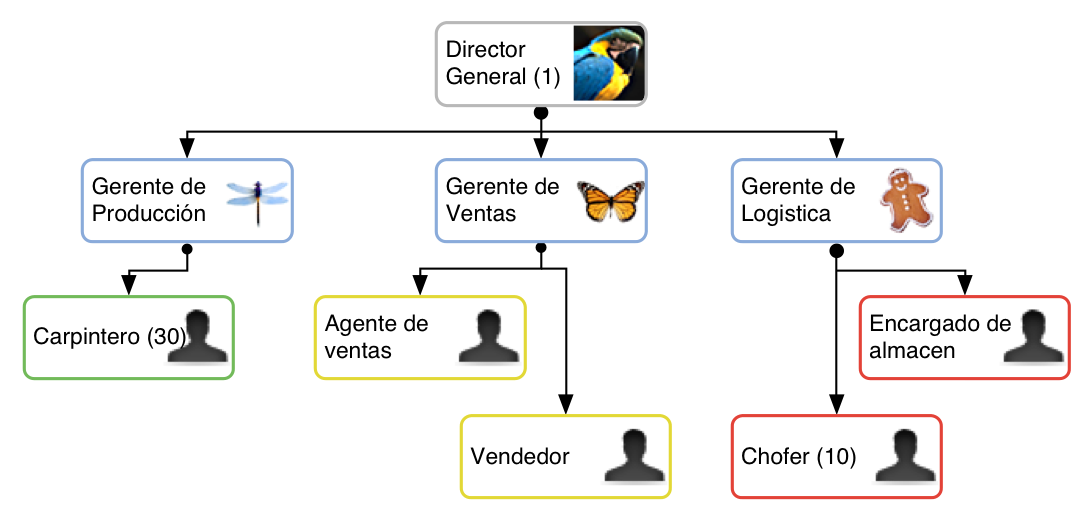
\includegraphics[width=.8\textwidth]{images/organigramaEm}
		\caption{Organigrama de la Mueblería Qetzal S. A. de C. V.}
		\label{fig:organigrama}
	\end{center}
\end{figure}


%---------------------------------------------------------
\section{Procesos involucrados}

\cdtInstrucciones{
	Coloque el mapa de procesos de la organización y liste a continuación los proceso que serán afectados por el desarrollo del sistema. Para cada proceso indique: Clave, Nombre y descripción.
}

\begin{figure}[htbp!]
	\begin{center}
		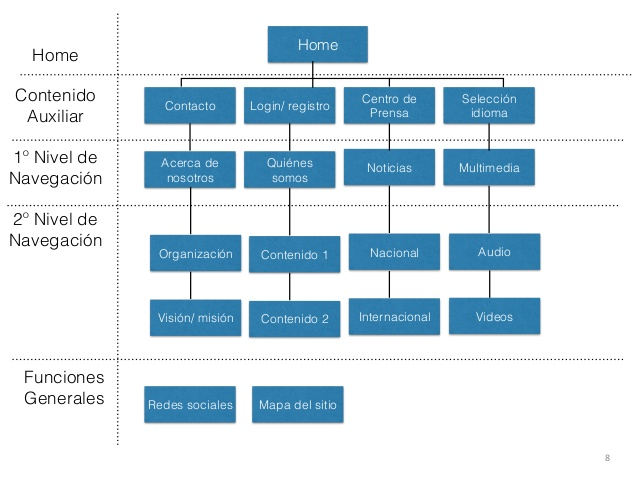
\includegraphics[width=.8\textwidth]{images/mapa}
		\caption{Mapa de procesos de la Mueblería Qetzal S. A. de C. V.}
		\label{fig:mapaProcASIS}
	\end{center}
\end{figure}

\begin{description}
	\item[PR-01] Nombre del proceso. Descripción del proceso.
\end{description}

%---------------------------------------------------------
\section{Requerimientos de usuario}

\cdtInstrucciones{
	Identifique y describa los requerimientos del usuario señalando: id, nombre, descripción y prioridad.
}

Los requerimientos del usuario son los siguientes\FootnoteStatus:

\begin{requerimientosU}
	\FRitem{RU-01}{Nombre del requerimiento}{Descripción del requerimiento.}{1}{\TODO}
	\FRitem{...}{...}{...}{...}{...}
\end{requerimientosU}

%---------------------------------------------------------
\section{Especificación de plataforma}	

\cdtInstrucciones{
	Coloque un diagrama y su descripción para aclarar el tipo de solución propuesta. \\
	
 En esta sección se debe aclarar:
	
\begin{description}
	\item[Tipo de sistema:] Web, aplicación móvil, de escritorio, híbrida, etc.
	\item[Software requerido:] Programas que se deberán instalar, desde el sistema operativo, compiladores, interpretes, servidores, etc.
	\item[Hardware requerido:] CPU, núcleos, velocidad, memoria, disco duro, etc.
	\item[servicios:] De conexión, seguridad, firewall, respaldo de energía, redundancia, uso de raids, etc.
\end{description}
}

\begin{figure}[htbp!]
	\begin{center}
		\fbox{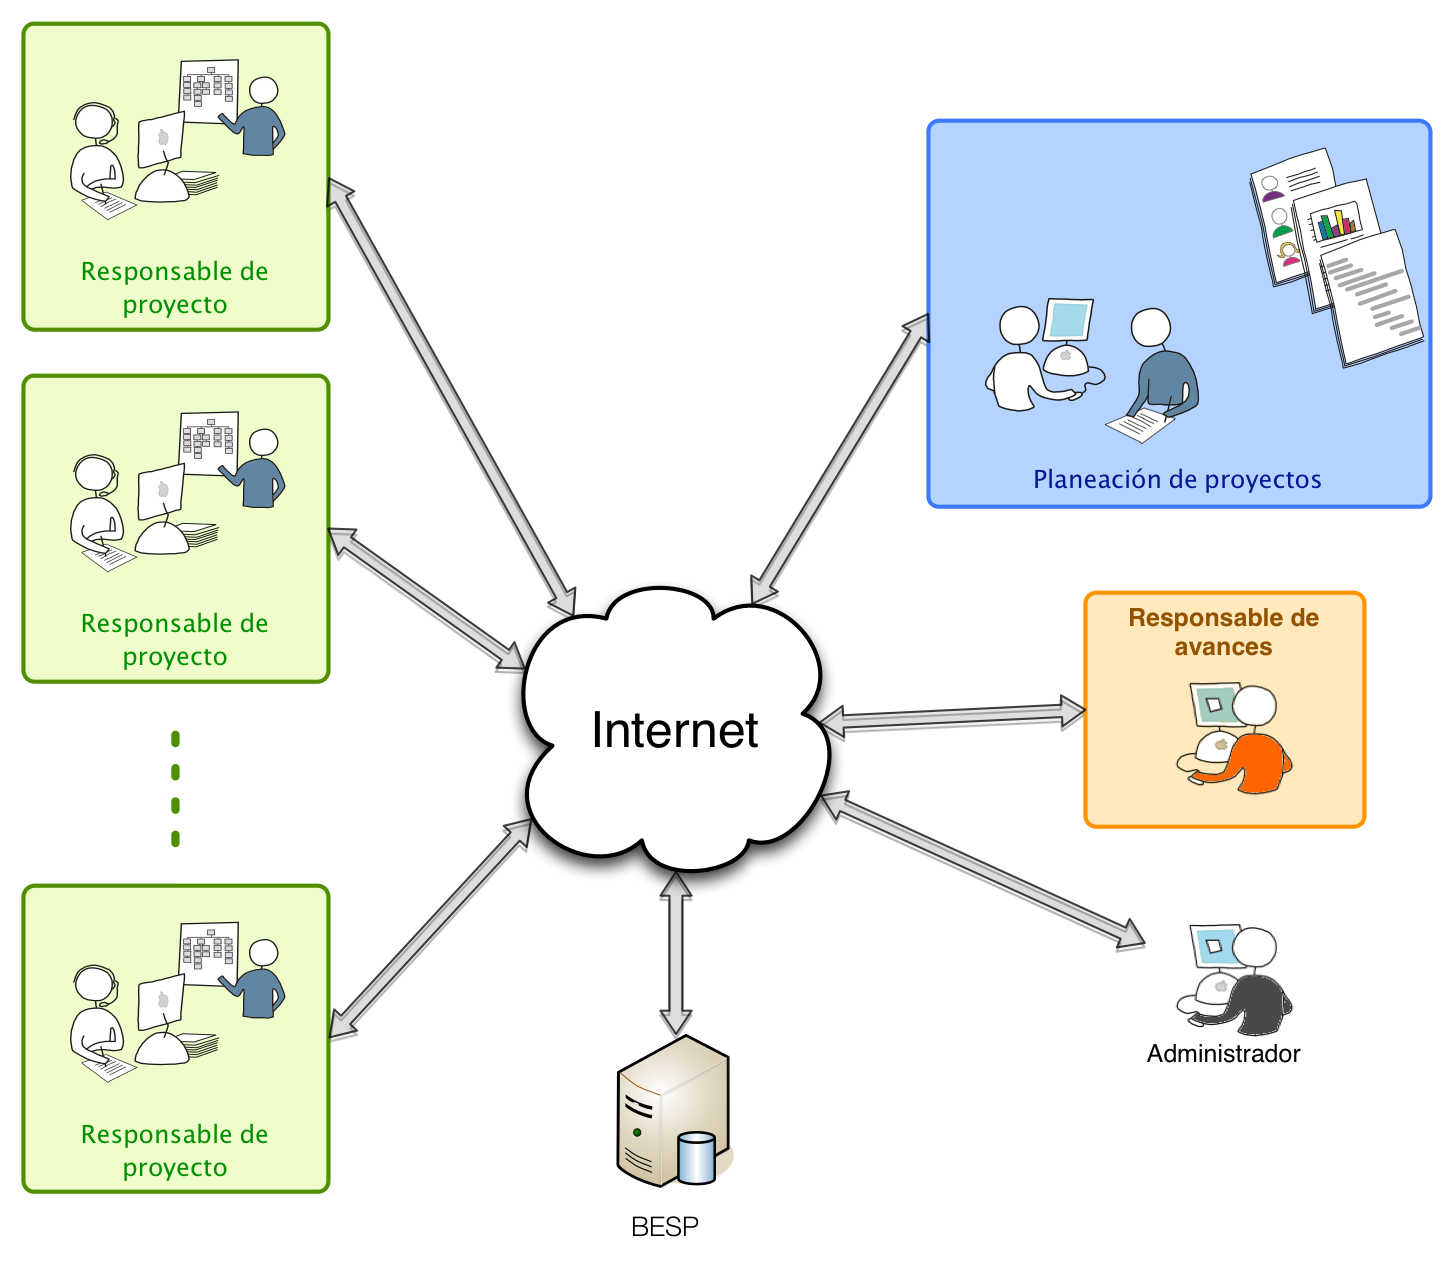
\includegraphics[width=.6\textwidth]{images/arquitectura}}
		\caption{Arquitectura del sistema.}
		\label{fig:arquitectura}
	\end{center}
\end{figure}

En la figura~\ref{fig:arquitectura} se describe la estructura del sistema, en ella se detalla ...




%=========================================================
% !TeX root = proyecto.tex

%=========================================================
\chapter{Modelo del Negocio}	
\label{cap:reqSist}

\cdtInstrucciones{Introduzca el capítulo describiendo el contenido del mismo, su organización y propósito.}

%----------------------------------------------------------
\section{Actores del sistema}

	\cdtInstrucciones{En esta sección describa a los actores del sistema.}
	
	%---------------------------------------------------------
	\begin{Usuario}{\hypertarget{Cliente}{\subsection{Cliente}}}{
			Es todo aquel actor que no pertenezca a la empresa y que desea desea reservar, hospedar y contratar los servicios que ofrece la empresa para su mascota.
		}
		\item[Responsabilidades:] \cdtEmpty
		\begin{itemize}
			\item Brindar datos precisos y actualizados de identificación de su persona y de su(s) mascota(s) para registrarse en el sistema y contratar los servicios que ofrece la empresa.
			\item Gestionar sus mascotas registradas en el sistema.
			\item Brindar datos precisos y actualizados de los medicamentos y vacunas administradas a su(s) mascota(s).
			\item Brindar datos actualizados de las noches, cuartos y servicios que desea reservar, así como las fechas de llegada (check-in) y salida (check-out) del hotel.
			\item Brindar datos precisos, actualizados y necesarios para pagar en el sistema por los servicios que se adquieran.
		\end{itemize}
		
		\item[Perfil:] \cdtEmpty
		\begin{itemize}
			\item Público mexicano que disponga de los recursos para cubrir el hospedaje de sus mascotas.
			\item Posée una o más mascotas a las que la empresa pueda ofrecer sus servicios.
		\end{itemize}
		\item[Procesos en los que participa:] \cdtEmpty
		\begin{itemize}
			%TODO: Agregar los procesos en los que se involucrará al cliente
			\item .
		\end{itemize}
	\end{Usuario}

	
%---------------------------------------------------------
\section{Términos del Negocio}
\label{sec:terminosDeNegocio}

\cdtInstrucciones{En esta sección describa todos los términos del negocio que aparecen en la especificación del sistema.}
	
\begin{description}
	% Ejemplo de un término literal.
	\item[\hypertarget{tAutomovil}{Automóvil:}] ({\em es un tipo de \hyperlink{tVehiculo}{Vehículo}}) De cuatro ruedas con capacidad de 5 a 9 personas. 
	% Ejemplo de un término de entidad
	\item[\hypertarget{tCliente}{Cliente:}] Se refiere a todas las personas físicas y morales que \hyperlink{tRenta}{rentan} o han rentado un \hyperlink{tVehiculo}{vehículo}.
	
	\item[\hypertarget{tDirector}{Director:}] ({\em es un tipo de \hyperlink{tEmpleado}{Empleado}}) Es el empleado que tiene mayor rango de todos y no tiene superior, a diferencia de los demás.	
	\item[\hypertarget{tEmpleado}{Empleado:}] Se refiere a cualquier persona que labore en la empresa.
	
	\item[\hypertarget{tChecador}{Checador:}] ({\em Reloj asociado al atributo:} Hora de entrada y salida de un \hyperlink{tEmpleado}{empleado}. {\em Frecuencia de lectura:} Una vez al día para la entrada y otra para la salida durante los días laborales.
	
	\item[\hypertarget{tMotocicleta}{Motocicleta:}] ({\em es un tipo de {tVehiculo}{Vehículo}}) De dos ruedas con capacidad para una personas. 

	\item[\hypertarget{tRenta}{Renta:}] Se refiere al servicio que ofrece la empresa para prestar \hyperlink{tVehiculo}{vehículos} a los \hyperlink{tCliente}{clientes} por un tiempo definido.
	
	\item[\hypertarget{tVehiculo}{Vehiculo:}] Se refiere a los automóviles y motocicletas que la empresa usa para dar el servicio de renta a los \hyperlink{tCliente}{clientes}.
	
%	\brTermSensor{tVelocimetro}{Velocímetro:}{Velocidad de un Vehículo.}{Kilometros/hora.}{Constantemente siempre que el \cdtRef{tVehiculo}{vehículo} esté encendido.}
\end{description}

%----------------------------------------------------------
\section{Modelo del dominio del problema}
\label{sec:hechosDeNegocio}

\cdtInstrucciones{En esta sección describa todas las entidades del negocio y sus relaciones.}

	El modelo del dominio del problema se muestra en la figura~\ref{fig:modeloDeDominio}, a continuación se describen cada una de las entidades y sus relaciones.
	
\begin{figure}[htpb!]
	\begin{center}
		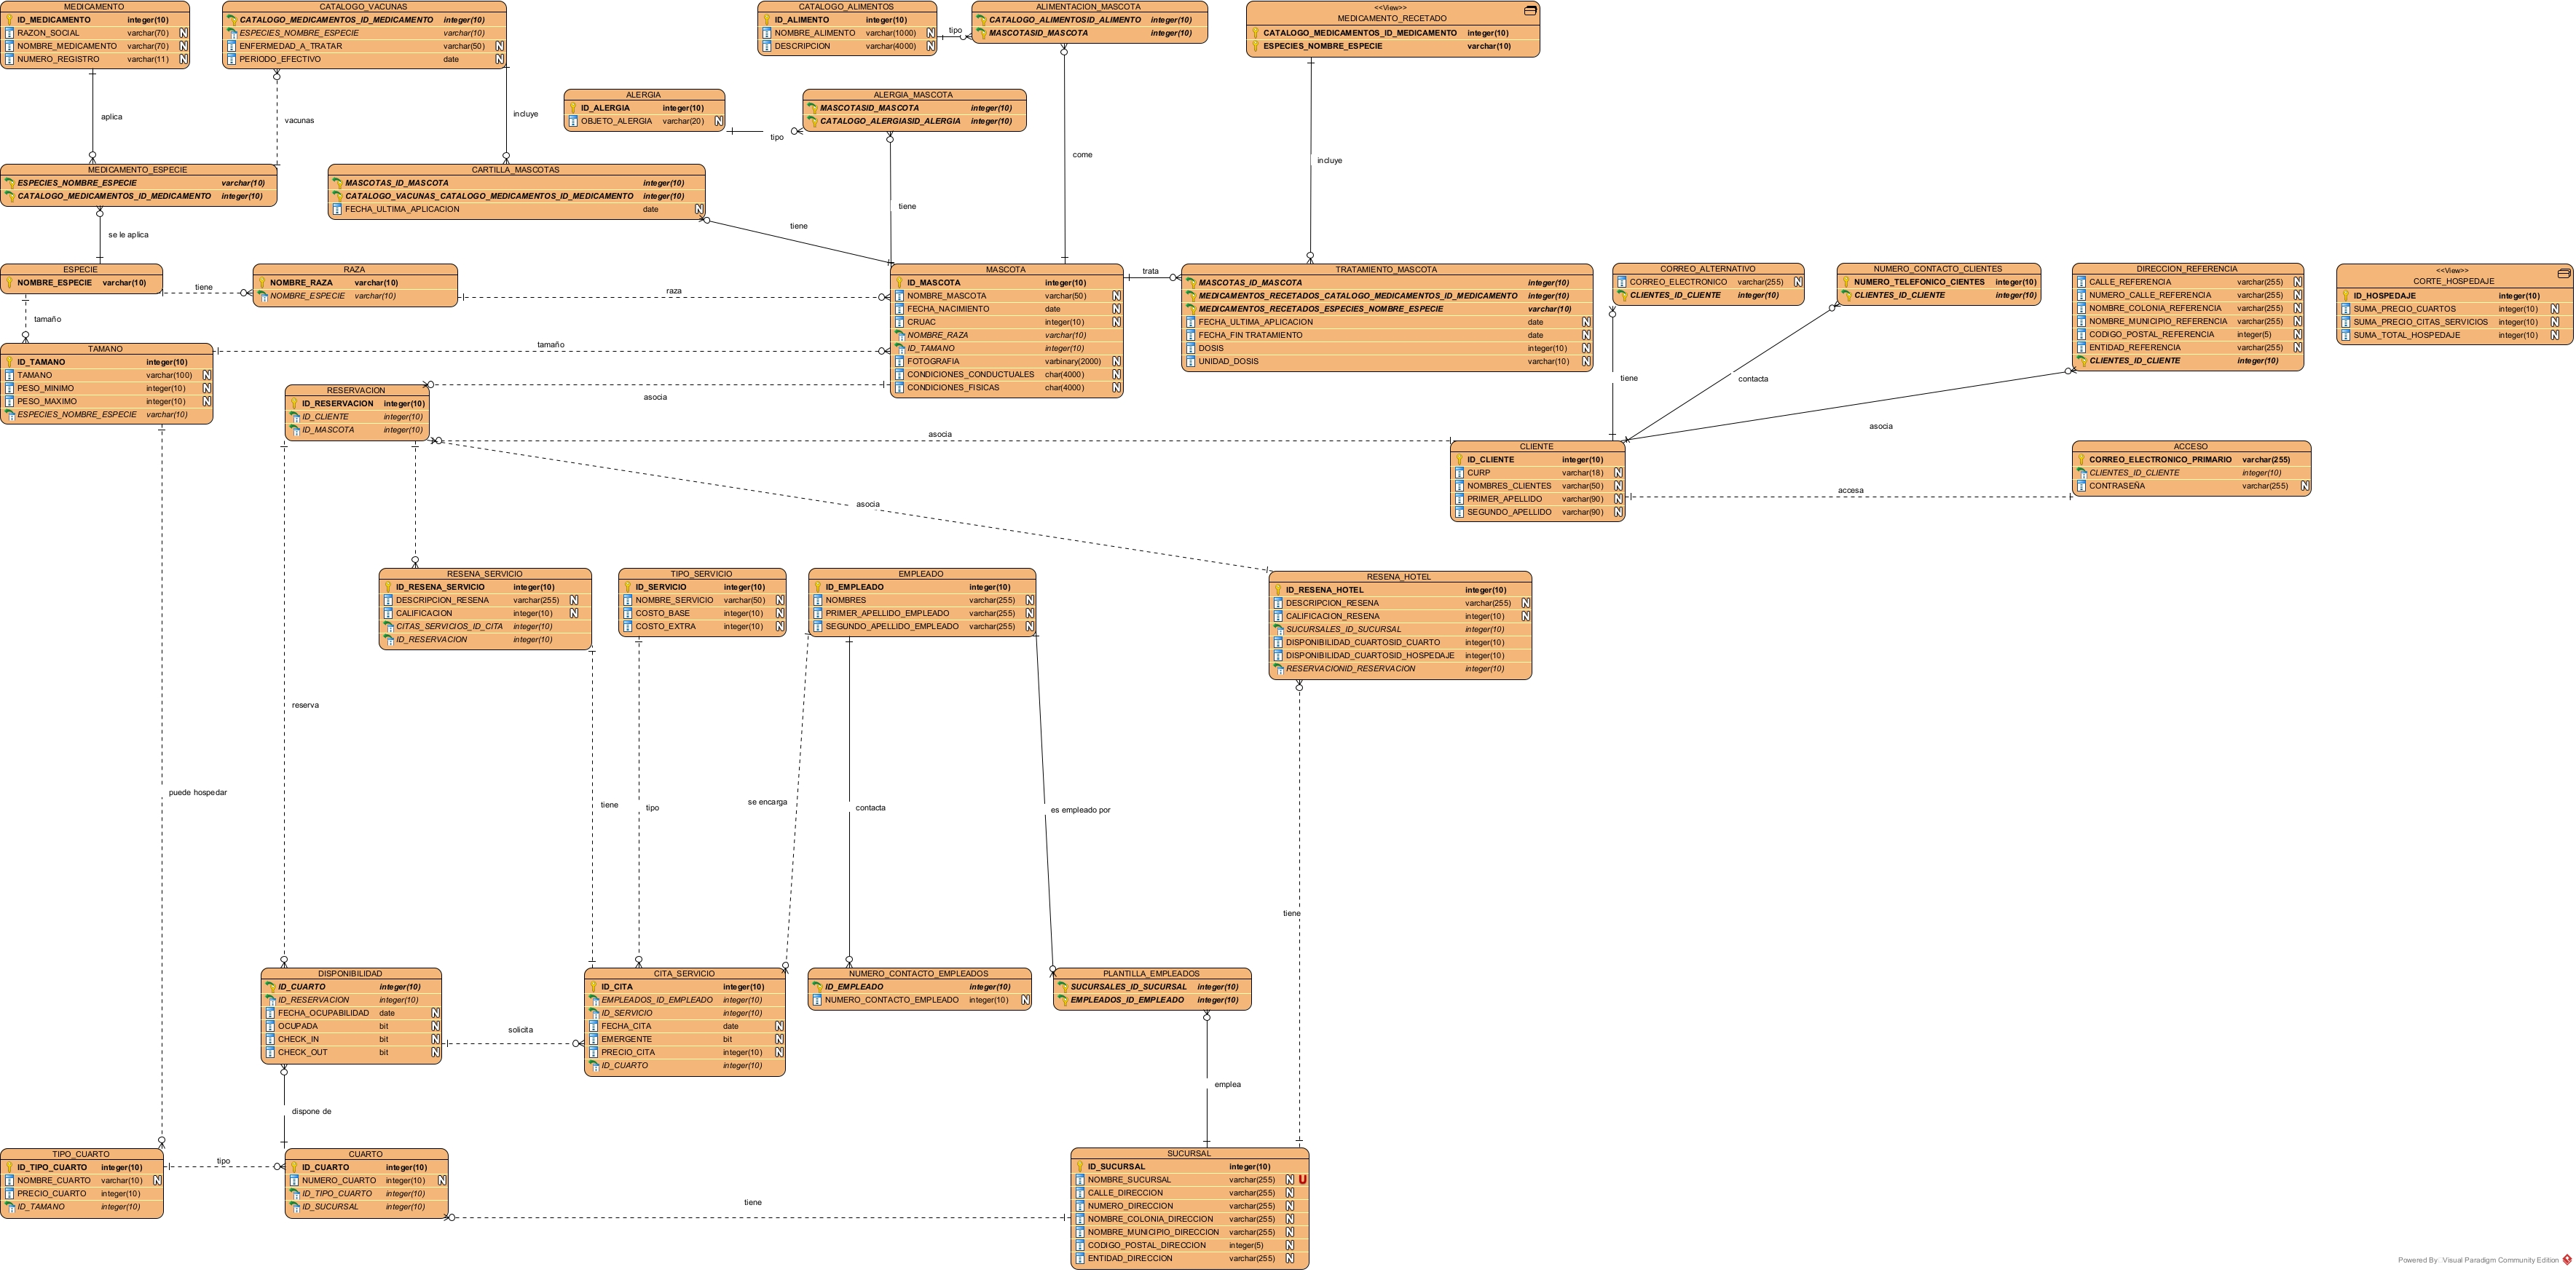
\includegraphics[angle=90,width=.60\textwidth]{images/Base_Datos}
		\caption{Modelo del dominio del problema}
		\label{fig:modeloDeDominio}
	\end{center}
\end{figure}

%\brRelComposition	Relación de composición
%\brRelAgregation	Relación de agregación
%\brRelGeneralization	Relación de generalización
%\brRelParticipation	Relación de participación
%- - - - - - - - - - - - - - - - - - - - - - - - - - - - - 
\begin{cdtEntidad}{mascota}{Mascota}%{}
	\brAttr{nombre}{Nombre}{Palabra Corta}
		{Nombre o nombres de la mascota.}{Sí}
	\brAttr{tamano}{Tamaño}{\hyperlink{tamanoMascota}{Tamaño mascota}}
		{Tamaño de la mascota.}{Sí}
	\brAttr{fechaNacimiento}{Fecha de Nacimiento}{date}
		{Fecha de nacimiento de la mascota.}{Sí}
	\brAttr{CRUAC}{CRUAC}{CURP}
		{CRUAC de la mascota.}{Sí}
	\brAttr{especie}{Especie}{\hyperlink{nombreEspecie}{Nombre especie}}
		{Especie de la mascota.}{Sí}
	\brAttr{raza}{Raza}{\hyperlink{nombreRaza}{Nombre raza}}
		{Raza de la mascota.}{Sí}
	\brAttr{foto}{Fotografia}{imagen}
		{Fotografia de la mascota.}{Sí}
	\brAttr{tipoVacuna}{Tipo de vacuna}{\hyperlink{vacunaMascota}{Vacuna mascota}}
		{Tipo de vacuna con la que cuenta la mascota.}{Sí}
	\brAttr{nombreVacuna}{Nombre de la vacuna}{Palabra corta}
		{Nombre de la vacuna con la que cuenta la mascota.}{Sí}
	\brAttr{fechaAplicacion}{Ultima fecha de aplicación}{date}
		{Ultima fecha de aplicación de la vacuna con la que cuenta la mascota.}{Sí}
	\brAttr{dosis}{Numero de dosis aplicadas}{Numero}
		{Numero de dosis aplicadas de la vacuna con la que cuenta la mascota.}{Sí}
	\brAttr{alergias}{Alergias}{\hyperlink{AlergiaMascota}{Alergia Mascota}}
		{Numero de dosis aplicadas de la vacuna con la que cuenta la mascota.}{Sí}
	\brAttr{tratamientoMedico}{Tratamiento Medico}{\hyperlink{tratamientoMedicoMascota}{Tratamiento medico mascota}}
		{Numero de dosis aplicadas de la vacuna con la que cuenta la mascota.}{Sí}
	\brAttr{caracteristicasEspeciales}{Caracteristicas Especiales}{varchar}
		{Caracteristicas especiales fisicas o de comportamiento de la mascota.}{Sí}
	%\cdtEntityRelSection
	%\brRel{\brRelAgregation}{País}{Un \hyperlink{Alumno}{Alumno} es originario de un \hyperlink{Pais}{Pais}}	
	%\brRel{\brRelGeneralization}{Alumno}{Un \hyperlink{AlumnoExtranjero}{Alumno Extranjero} es un  \hyperlink{Alumno}{Alumno}}	
	%\brRel{\brRelParticipation}{Alumno}{Un \hyperlink{AlumnoExtranjero}{Alumno Extranjero} es un  \hyperlink{Alumno}{Alumno}}	
\end{cdtEntidad}

\begin{cdtEntidad}{SUCURSAL}{Sucursal}
	\brAttr{ID_SUCURSAL}{ID de la sucursal}{ID}{ID interno asignado a cada sucursal.}{Sí}
	\brAttr{NOMBRE_SUCURSAL}{Nombre de la sucursal}{Cadena}{Nombre comercial de la sucursal.}{Sí}
	\brAttr{CALLE_DIRECCION}{Nombre de calle}{Cadena}{Calle de la dirección de la sucursal.}{Sí}
	\brAttr{NUMERO_DIRECCION}{Número de calle}{Cadena corta}{Número de calle de la dirección de la sucursal.}{Sí}
	\brAttr{NOMBRE_COLONIA_DIRECCION}{Nombre de colonia}{Frase corta}{Nombre de la colonia donde se ubica la sucursal.}{Sí}
	\brAttr{NOMBRE_MUNICIPIO_DIRECCION}{Nombre de municipio}{Frase corta}{Nombre del municipio donde se encuentra la sucursal.}{Sí}
	\brAttr{CODIGO_POSTAL_DIRECCION}{Código postal}{Numérico}{Código postal de la sucursal.}{Sí}
	\brAttr{ENTIDAD_DIRECCION}{Nombre de entidad}{Frase corta}{Entidad o estado donde se encuentra la sucursal.}{Sí}
	\cdtEntityRelSection
	\brRel{\brRelComposition}{Cuarto}{Una \hyperlink{SUCURSAL}{sucursal} tiene uno o más \hyperlink{CUARTO}{cuartos} en los que puede hospedar las mascotas de sus clientes.}
	\brRel{\brRelAgregation}{Empleado}{Una \hyperlink{SUCURSAL}{sucursal} tiene uno o más \hyperlink{EMPLEADO}{empleados} que trabajan en ella.}
	\brRel{\brRelComposition}{Reseña del hotel}{Una \hyperlink{SUCURSAL}{sucursal} tiene uno o más \hyperlink{RESENA_HOTEL}{reseñas} que califican sus estancias.}
\end{cdtEntidad}
%- - - - - - - - - - - - - - - - - - - - - - - - - - - - - 
\begin{cdtEntidad}{MEDICAMENTO}{Medicamento}
	\brAttr{ID_MEDICAMENTO}{ID del medicamento}{ID}{ID interno del medicamento de uso veterinario registrado en catálogos oficiales.}{Sí}
	\brAttr{RAZON_SOCIAL}{Razón social}{Frase}{Razón social de la empresa que desarrolló y produce el medicamento.}{Sí}
	\brAttr{NOMBRE_MEDICAMENTO}{Nombre del medicamento}{Frase}{Nombre comercial del medicamento.}{Sí}
	\brAttr{NUMERO_REGISTRO}{Número de registro}{ID}{Número de registro del medicamento en catálogos oficiales.}{Sí}
	\cdtEntityRelSection
	\brRel{\brRelComposition}{Especie}{Un \hyperlink{MEDICAMENTO}{medicamento} tiene una o más \hyperlink{ESPECIE}{especies} en las que se puede aplicar.}
\end{cdtEntidad}

%- - - - - - - - - - - - - - - - - - - - - - - - - - - - - 
\begin{cdtEntidad}{ESPECIE}{Especie}
	\brAttr{NOMBRE_ESPECIE}{Nombre de la especie}{Cadena}{Nombre de la especie de las mascotas.}{Sí}
	\cdtEntityRelSection
	\brRel{\brRelComposition}{Medicamento}{Una \hyperlink{ESPECIE}{especie} puede o no tener uno o más \hyperlink{MEDICAMENTO}{medicamentos} que se le pueden aplicar.}
	\brRel{\brRelGeneralization}{Raza}{Una \hyperlink{ESPECIE}{especie} tiene una o más \hyperlink{RAZA}{razas}.}
	\brRel{\brRelGeneralization}{Tamaño}{Una \hyperlink{ESPECIE}{especie} tiene uno o más \hyperlink{TAMANO}{tamaños}.}
	\brRel{\brRelAgregation}{Tipo de cuarto}{Un \hyperlink{TAMANO}{tamaño} de mascota puede o no tener uno o más \hyperlink{TIPO_CUARTO}{tipos de cuarto} en los que se puede hospedar.}
\end{cdtEntidad}

%- - - - - - - - - - - - - - - - - - - - - - - - - - - - - 
\begin{cdtEntidad}{RAZA}{Raza}
	\brAttr{NOMBRE_RAZA}{Nombre de la raza}{Cadena}{Nombre de la raza de las mascotas.}{Sí}
	\brAttr{NOMBRE_ESPECIE}{Nombre de la especie}{Palabra corta}{Nombre de la especie a la que pertenece la raza.}{Sí}
	\cdtEntityRelSection
	\brRel{\brRelComposition}{Mascota}{Una \hyperlink{ESPECIE}{raza} está asociado a una o más \hyperlink{MASCOTA}{mascotas}.}
\end{cdtEntidad}

%- - - - - - - - - - - - - - - - - - - - - - - - - - - - - 
\begin{cdtEntidad}{DISPONIBILIDAD_CUARTOS}{Disponibilidad de cuartos}
	\brAttr{ID_CUARTO}{ID del cuarto}{ID}{ID interno del cuarto en le que reservan.}{Sí}
	\brAttr{ID_HOSPEDAJE}{ID del hospedaje}{ID}{ID interno del hospedaje o estancia.}{No}
	\brAttr{ID_RESERVACION}{ID de reservación}{ID}{ID interno de la reservación que le corresponde a la estancia.}{Sí}
	\brAttr{FECHA_OCUPABILIDAD}{Fecha}{Fecha}{Fecha de disponibilidad.}{Sí}
	\brAttr{OCUPADA}{Ocupabilidad}{Booleano}{Indica si el cuarto está ocupado.}{Sí}
	\brAttr{CHECK-IN}{Check-in}{Booleano}{Indica si la fecha es el check-in.}{Sí}
	\brAttr{CHECK-OUT}{Check-out}{Booleano}{Indica si la fecha es el check-out.}{Sí}
	\brAttr{CHECK-IN}{Check-in}{Booleano}{Indica si el cuarto está ocupado.}{Sí}
	\cdtEntityRelSection
	\brRel{\brRelParticipation}{Reseña de servicio}{Un \hyperlink{TIPO_CUARTO}{tipo de cuarto} puede estar asociado a uno o más
\hyperlink{CUARTO}{cuartos}.}
\end{cdtEntidad}

%- - - - - - - - - - - - - - - - - - - - - - - - - - - - - 
\begin{cdtEntidad}{TIPO_CUARTO}{Tipo de cuarto}
	\brAttr{ID_TIPO_CUARTO}{ID del tipo de cuarto}{ID}{ID interno del tipo de cuarto que tienen todos los hoteles.}{Sí}
	\brAttr{NOMBRE_CUARTO}{Nombre del cuarto}{Frase corta}{Nombre comercial del tipo de cuarto del que dispone el hotel en al menos una o más sucursales.}{Sí}
	\brAttr{PRECIO_CUARTO}{Precio del cuarto}{Numérico con decimales}{Precio establecido para el tipo de cuarto.}{Sí}
	\brAttr{ID_TAMANO}{ID tamaño}{ID}{ID del tamaño asociado que puede hospedar el cuarto.}{Sí}
	\cdtEntityRelSection
	\brRel{\brRelGeneralization}{Cuarto}{Un \hyperlink{TIPO_CUARTO}{tipo de cuarto} puede estar asociado a uno o más
\hyperlink{CUARTO}{cuartos}.}
\end{cdtEntidad}


%- - - - - - - - - - - - - - - - - - - - - - - - - - - - - 
\begin{cdtEntidad}{ACCESO}{Acceso}
	\brAttr{ID_CLIENTES_CLIENTE}{ID Cliente}{ID}
		{ID del cliente al que corresponden las credenciales.}{Sí}
	\brAttr{CONTRASENA}{Contraseña}{Cadena corta}
		{Contraseña para accesar al perfil.}{Sí}
	\brAttr{COREO_ELECTRONICO_PRIMARIO}{Correo electrónico primario}{Correo}
		{Correo principal con el que se identifica el cliente.}{Sí}
	\cdtEntityRelSection
	\brRel{\brRelComposition}{ID Cliente}{Un \hyperlink{Alumno}{ID} reside en un \hyperlink{Domicilio}{Domicilio}.}	
	\brRel{\brRelAgregation}{Grupo}{Un \hyperlink{Alumno}{Alumno} toma un \hyperlink{Curso}{Curso}.}	
\end{cdtEntidad}

%- - - - - - - - - - - - - - - - - - - - - - - - - - - - - 
\begin{cdtEntidad}{CLIENTES}{Alumno Extranjero}%{}
	\brAttr{numeroResidente}{Numero de residente}{Id}{Número de registro dado por la Secretaría de Relaciones Exteriores a los extranjeros.}{Si}
	\brAttr{paisOrigen}{Pais origen}{\hyperlink{Pais}{País}}
		{País de origen del alumno extranjero.}{Sí}
	\cdtEntityRelSection
	\brRel{\brRelAgregation}{País}{Un \hyperlink{Alumno}{Alumno} es originario de un \hyperlink{Pais}{Pais}}	
	\brRel{\brRelGeneralization}{Alumno}{Un \hyperlink{AlumnoExtranjero}{Alumno Extranjero} es un  \hyperlink{Alumno}{Alumno}}	
	\brRel{\brRelParticipation}{Alumno}{Un \hyperlink{AlumnoExtranjero}{Alumno Extranjero} es un  \hyperlink{Alumno}{Alumno}}	
\end{cdtEntidad}

%---------------------------------------------------------
\section{Modelado de Reglas de negocio}


% !TeX root = proyecto.tex


\cdtInstrucciones{En esta sección describa todas las reglas de negocio identificadas.}


% Tipo: \btDerivation (no aplica Clase), \btEnabler, \btTimer, \btExecutive
% Clase: \bcCondition, \bcIntegrity, \bcAutorization.
% Cumplimiento: \blStrict \blDeferred \blPreAutorized \blPostJustified \blOverride \blGuideline
\begin{BussinesRule}[%
	\brClassification{\btEnabler}{\bcCondition}{\blStrict}
	]{BR-001}{Nombre de la regla de negocio}
	
				% Opciones para nivel: \blControlling, \blInfluencing
	\BRitem[Descripción:] Descripción de la regla. Forma coloquial a manera de reglamento.
	\BRitem[Motivación:] Describa por que es importante la regla.
	\BRitem[Sentencia:] Sentencia formal de la regla.
	\BRitem[Ejemplo positivo:] Indique uno o varios ejemplos en donde la regla se cumple.
        \begin{itemize}
        	\item ...
        \end{itemize}
	
	\BRitem[Ejemplo negativo:] Indique uno o varios ejemplos en dónde la regla no se cumple.
		\begin{itemize}
        	\item ...
        \end{itemize}
	
	\BRitem[Referenciado por:] Liste los casos de uso en donde la regla no se cumple. por ejemplo \hyperlink{CUCE3.2}{CUCE3.2}, \hyperlink{CUCE3.3}{CUCE3.3}.
\end{BussinesRule}


\begin{BussinesRule}[%Cambiar el nivel de la regla a \blPostJustified
	\brClassification{\btEnabler}{\bcCondition}{\blStrict}
	]{BR-002}{Vacunas Obligatorias para la Mascota}
	\BRitem[Descripción:] Para que una mascota pueda hacer uso de las instalaciones del hotel, debe contar con las 3 vacunas obligatorias: Rabia, Bordetella, Leptospirosis
%En la PROFECO menciona que para perros deben ser: parvovirus canino, moquillo, hepatitis canina y la rabia, para gatos: Rabia, Trivalente para rinotraqueitis, calicivirus y panleucopenia y leucemia felina. La vacunación para hurones y conejos es cubierta con la de gatos. Para cerdos: parvovirus, erysipelothrix rhusiopathiae y aujeszky.
	\BRitem[Motivación:] Al darse la convivencia entre especies y distintos estilos de vida, es mandatorio legalmente la aplicaciones de determinadas vacunas en función de la especie para garantizar seguridad sanitaria a todos los huéspedes y sus dueños.
	\BRitem[Sentencia:] Sea $a$ una mascota, $Especies$ el conjunto de especies que puede hospedar el hotel, $Hospedados$ el conjunto de mascotas que hospeda el hotel, $Vacunas$ el conjunto de vacunas aplicables a culquier mascota, $Obligatorias$ el subconjunto de $Vacunas$ ($Obligatorias\subset Vacunas$) de vacunas obligatorias, $ultimaAplicacion$ la fecha de la última aplicación de la vacuna, $fechaHospedaje$ la fecha en la que iniciará su hospedaje y $periodoVigente$ el tiempo de vigencia de la vacuna; $a \in Hospedados \iff a\in (Especies\cap  Obligatorias) \land (fechaHospedaje - ultimaAplicacion < periodoVigencia)$, es decir, una mascota estará hospedada si y solo si pertenece al conjunto de especies con vacunas obligatorias aplicadas y la diferencia de la fecha del check-in y la de aplicación de la vacuna sea menor al periodo de vigencia de la vacuna misma.
	\BRitem[Ejemplo positivo:] El perro Rufus es hospedado ya que cuenta con las vacunas :
	\begin{itemize}
        		\item Rabia: aplicada hace 2 meses.
		\item Bordetella: aplicada hace 3 meses.
		\item Leptospirosis: hace 4 meses .
	\end{itemize}
	
	\BRitem[Ejemplo negativo:] El perro Alemán no es hospedado ya que solo cuenta con las vacunas:
	\begin{itemize}
        		\item Rabia: aplicada hace 12 meses.
		\item Bordetella: aplicada hace 14 meses.
	\end{itemize}
	necesitando una consulta con el médico veterinario
	
	\BRitem[Referenciado por:] \hyperlink{CU3}{CU3}.
\end{BussinesRule}


\section{Máquinas de estado}

% !TeX root = proyecto.tex

\cdtInstrucciones{En esta sección describa para cada máquina de estados y a que entidad corresponde. Utilice reglas ECA en el diagrama y elabore el diagrama de estados, una descripción del diagrama, una descripción de cada estado y una descripción de las acciones indicando que casos de uso están involucrados.}

% - - - - - - - - - - - - - - - - - - - - - - - - - - - - 
\subsection{Estados para un préstamo}

En la figura~\ref{fig:edos-prestamo} se muestran ...

\begin{figure}[htbp]
	\begin{center}
		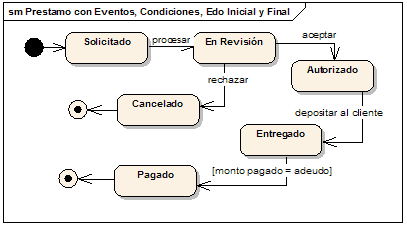
\includegraphics[width=.7\textwidth]{images/edoPrestamo}
		\caption{Máquina de estados de un Préstamo.}
		\label{fig:edos-prestamo}
	\end{center}
\end{figure}

\subsubsection{Estados}

\begin{description}
	\item[Estado:] Descripción del estado.
	\item[...] ...
\end{description}


\subsubsection{Acciones}

\begin{description}
	\item[Acción:] Descripción de la acción indicando el Caso de uso involucrado.
	\item[...] ...
\end{description}


%---------------------------------------------------------
\section{Modelo de Procesos AS-IS}

\cdtInstrucciones{En esta seccion describa todos los procesos tal cual son antesd e desarrollar el proyecto.}

En esta sección se describen los procesos a mejorar con el sistema. En la figura~\ref{fig:mapaProc} se muestra el mapa de procesos y se indican los proceso afectados por el sistema.

\begin{figure}[htbp]
	\begin{center}
		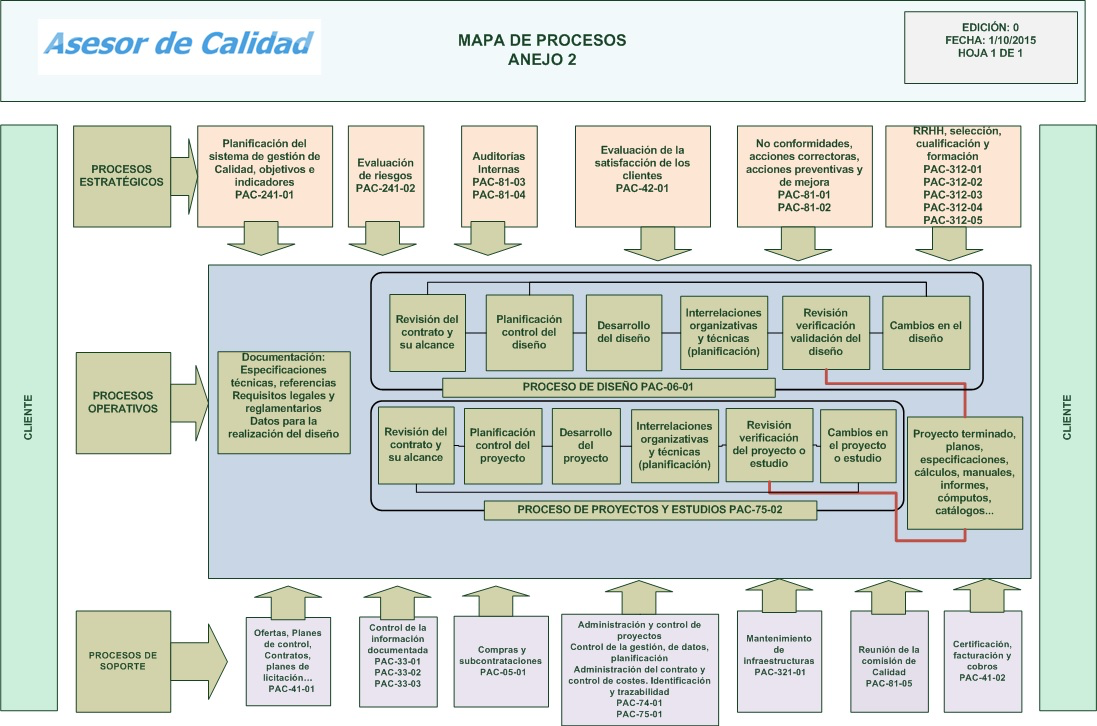
\includegraphics[width=.8\textwidth]{images/mapaProc}
		\caption{Mapa de procesos actual.}
		\label{fig:mapaProc}
	\end{center}
\end{figure}

% !TeX root = ../proyecto.tex




% - - - - - - - - - - - - - - - - - - - - - - - - - - - - 
\subsection{PROC-01 Nombre del proceso}

\begin{figure}[htbp]
	\begin{center}
		
\includegraphics[width=.7\textwidth]{images/proceso1}
		\caption{PROC-01 Proceso de Análisis de requerimientos}
		\label{fig:proceso1}
	\end{center}
\end{figure}

\begin{description}
	\item[Descripción:] Describa el proceso indicando los aspectos relevantes que el diagrama no muestra.
	\item[Entradas:] \cdtEmpty
        \begin{itemize}
			\item Documentos de Procesos.
			\item Reglas de negocio.
			\item Minutas de las reuniones de análisis.
        \end{itemize}
	\item[Salidas:] \cdtEmpty
        \begin{itemize}
			\item Especificación de requerimientos.
			\item Bosquejo de pantallas.
			\item Modelo de base de datos
        \end{itemize}	
    \item[Áreas de oportunidad:] Liste los aspectos que detecta se pueden mejorar con la introducción del sistema o los problemas encontrados.
\end{description}

%\input{proc/proc02.tex}
%\input{proc/proc03.tex}
%\input{proc/proc04.tex}

%---------------------------------------------------------
\section{Modelo de procesos TO-BE}

\cdtInstrucciones{En esta seccion describa todos los procesos modificados una vez que se adopte el sistema.}

Los nuevos procesos se presentan en esta sección, el mapa de procesos de la figura~\ref{fig:mapaProcNvo} se muestra el mapa de procesos actualizado.

\begin{figure}[htbp]
	\begin{center}
		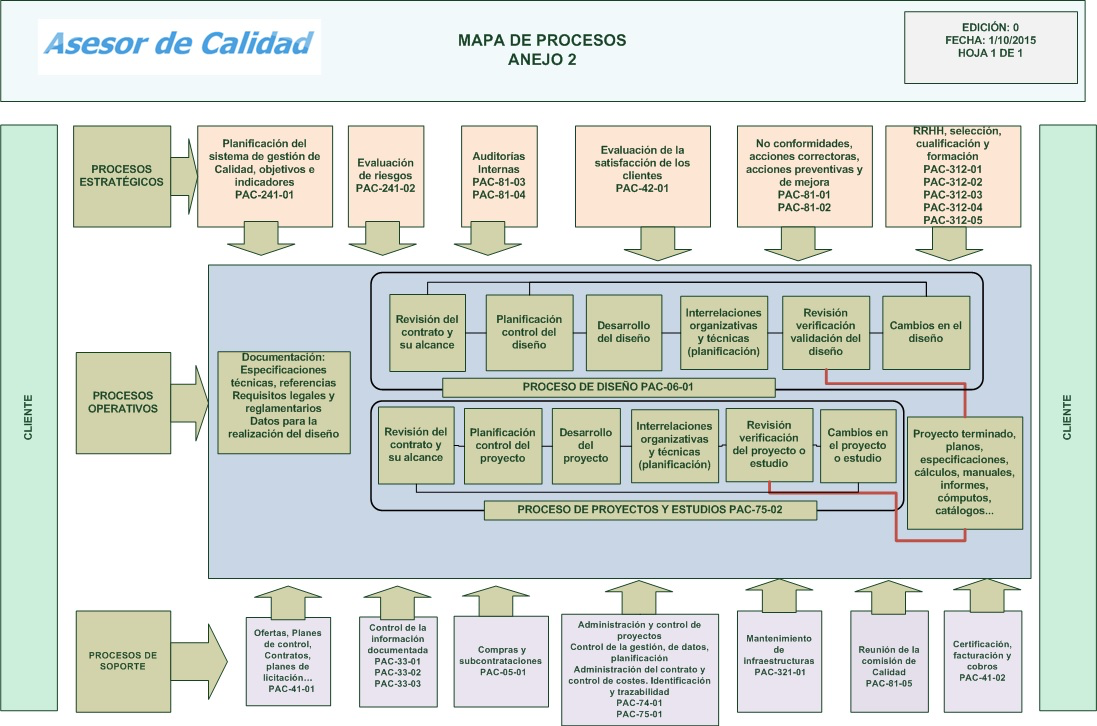
\includegraphics[width=.8\textwidth]{images/mapaProc}
		\caption{Mapa de procesos actualizado}
		\label{fig:mapaProcNvo}
	\end{center}
\end{figure}


% - - - - - - - - - - - - - - - - - - - - - - - - - - - - 
\subsection{PROCM-01 ...}

\begin{figure}[htbp]
	\begin{center}
		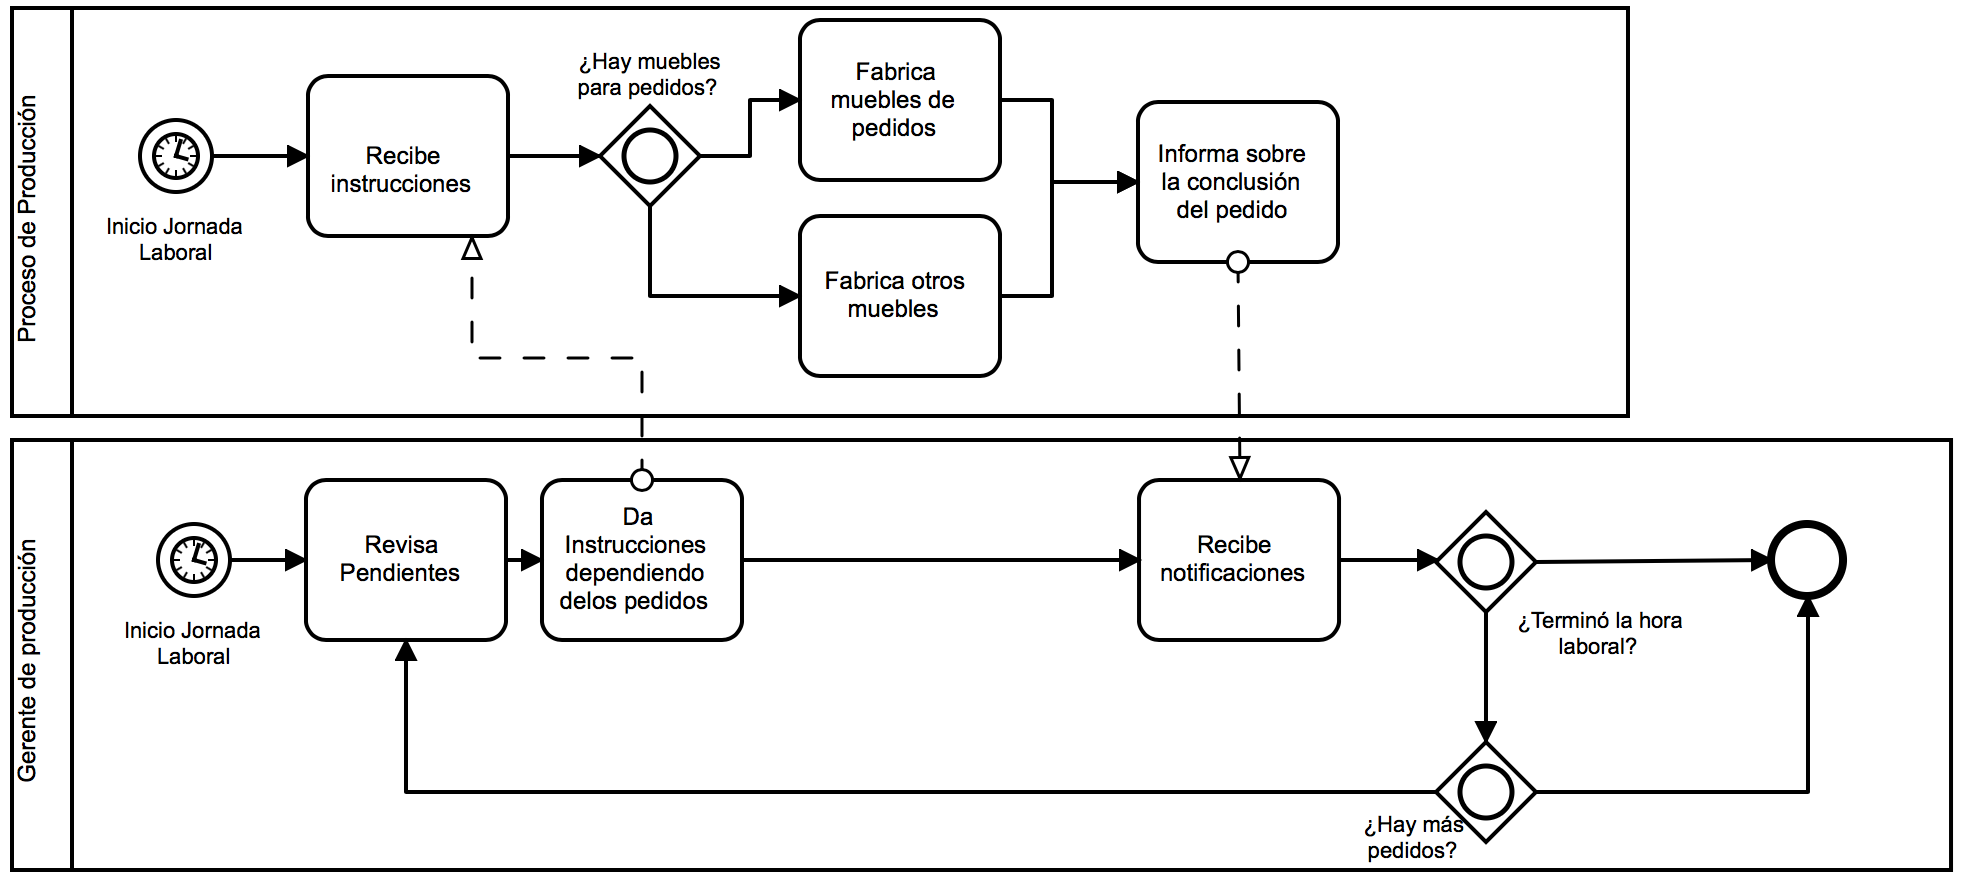
\includegraphics[width=.8\textwidth]{images/proceso3}
		\caption{PROCM-01 Nombre del proceso}
		\label{fig:proceso3}
	\end{center}
\end{figure}

\begin{description}
	\item[Descripción:] ...
	\item[Entradas:] \cdtEmpty
        \begin{itemize}
			\item ...
        \end{itemize}
	\item[Salidas:] \cdtEmpty
        \begin{itemize}
			\item ...
        \end{itemize}	
    \item[Mejoras esperadas:] Liste las mejoras que espera obtener tras la implementación del sistema.
    \item[Reglas de negocio:] \hyperlink{BR05}{BR05}, \hyperlink{BR8}{BR8}.
    \item[Casos de uso:] \hyperlink{CU3.4}{CU 3.4 Login}, \hyperlink{CU 4.3}{ CU 4.3 Consultar productos}.
\end{description}

%\input{proc/proc-m02.tex}
%\input{proc/proc-m03.tex}
%\input{proc/proc-m04.tex}



%=========================================================
% !TeX root = proyecto.tex

%=========================================================
\chapter{Modelo dinámico}	
\label{cap:modDinamico}

\cdtInstrucciones{Presente la solución indicando el si esta se compone de varios sistemas, los subsistemas del sistema y si aplica, los módulos de los subsistemas.}

	Este capítulo describe en modelo dinámico del sistema. en el se detallan todos los escenarios de ejecución del sistema. La figura~\ref{fig:casosDeUso} muestra el diagrama general del sistema y sus subsistemas, y la figura~\ref{fig:casosDeUsoDetalle} muestra todos los casos de uso del sistema. En este documento solo detallamos los casos de uso del subsistema de gestión de cursos.
	
\begin{figure}[htbp]
	\begin{center}
		\fbox{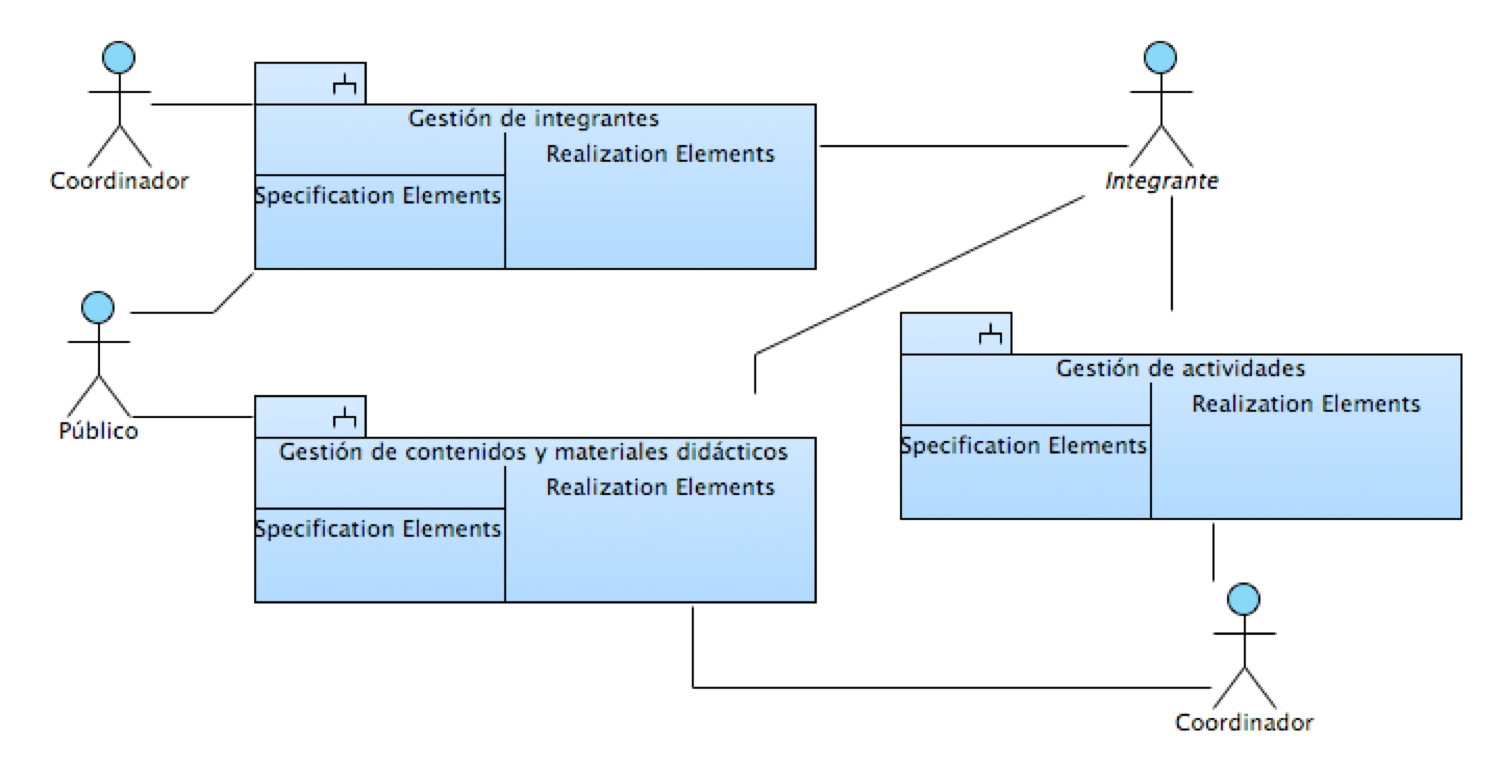
\includegraphics[width=.8\textwidth]{images/casosDeUso}}
		\caption{Diagrama de casos de uso del sistema.}
		\label{fig:casosDeUso}
	\end{center}
\end{figure}

\begin{figure}[htbp]
	\begin{center}
		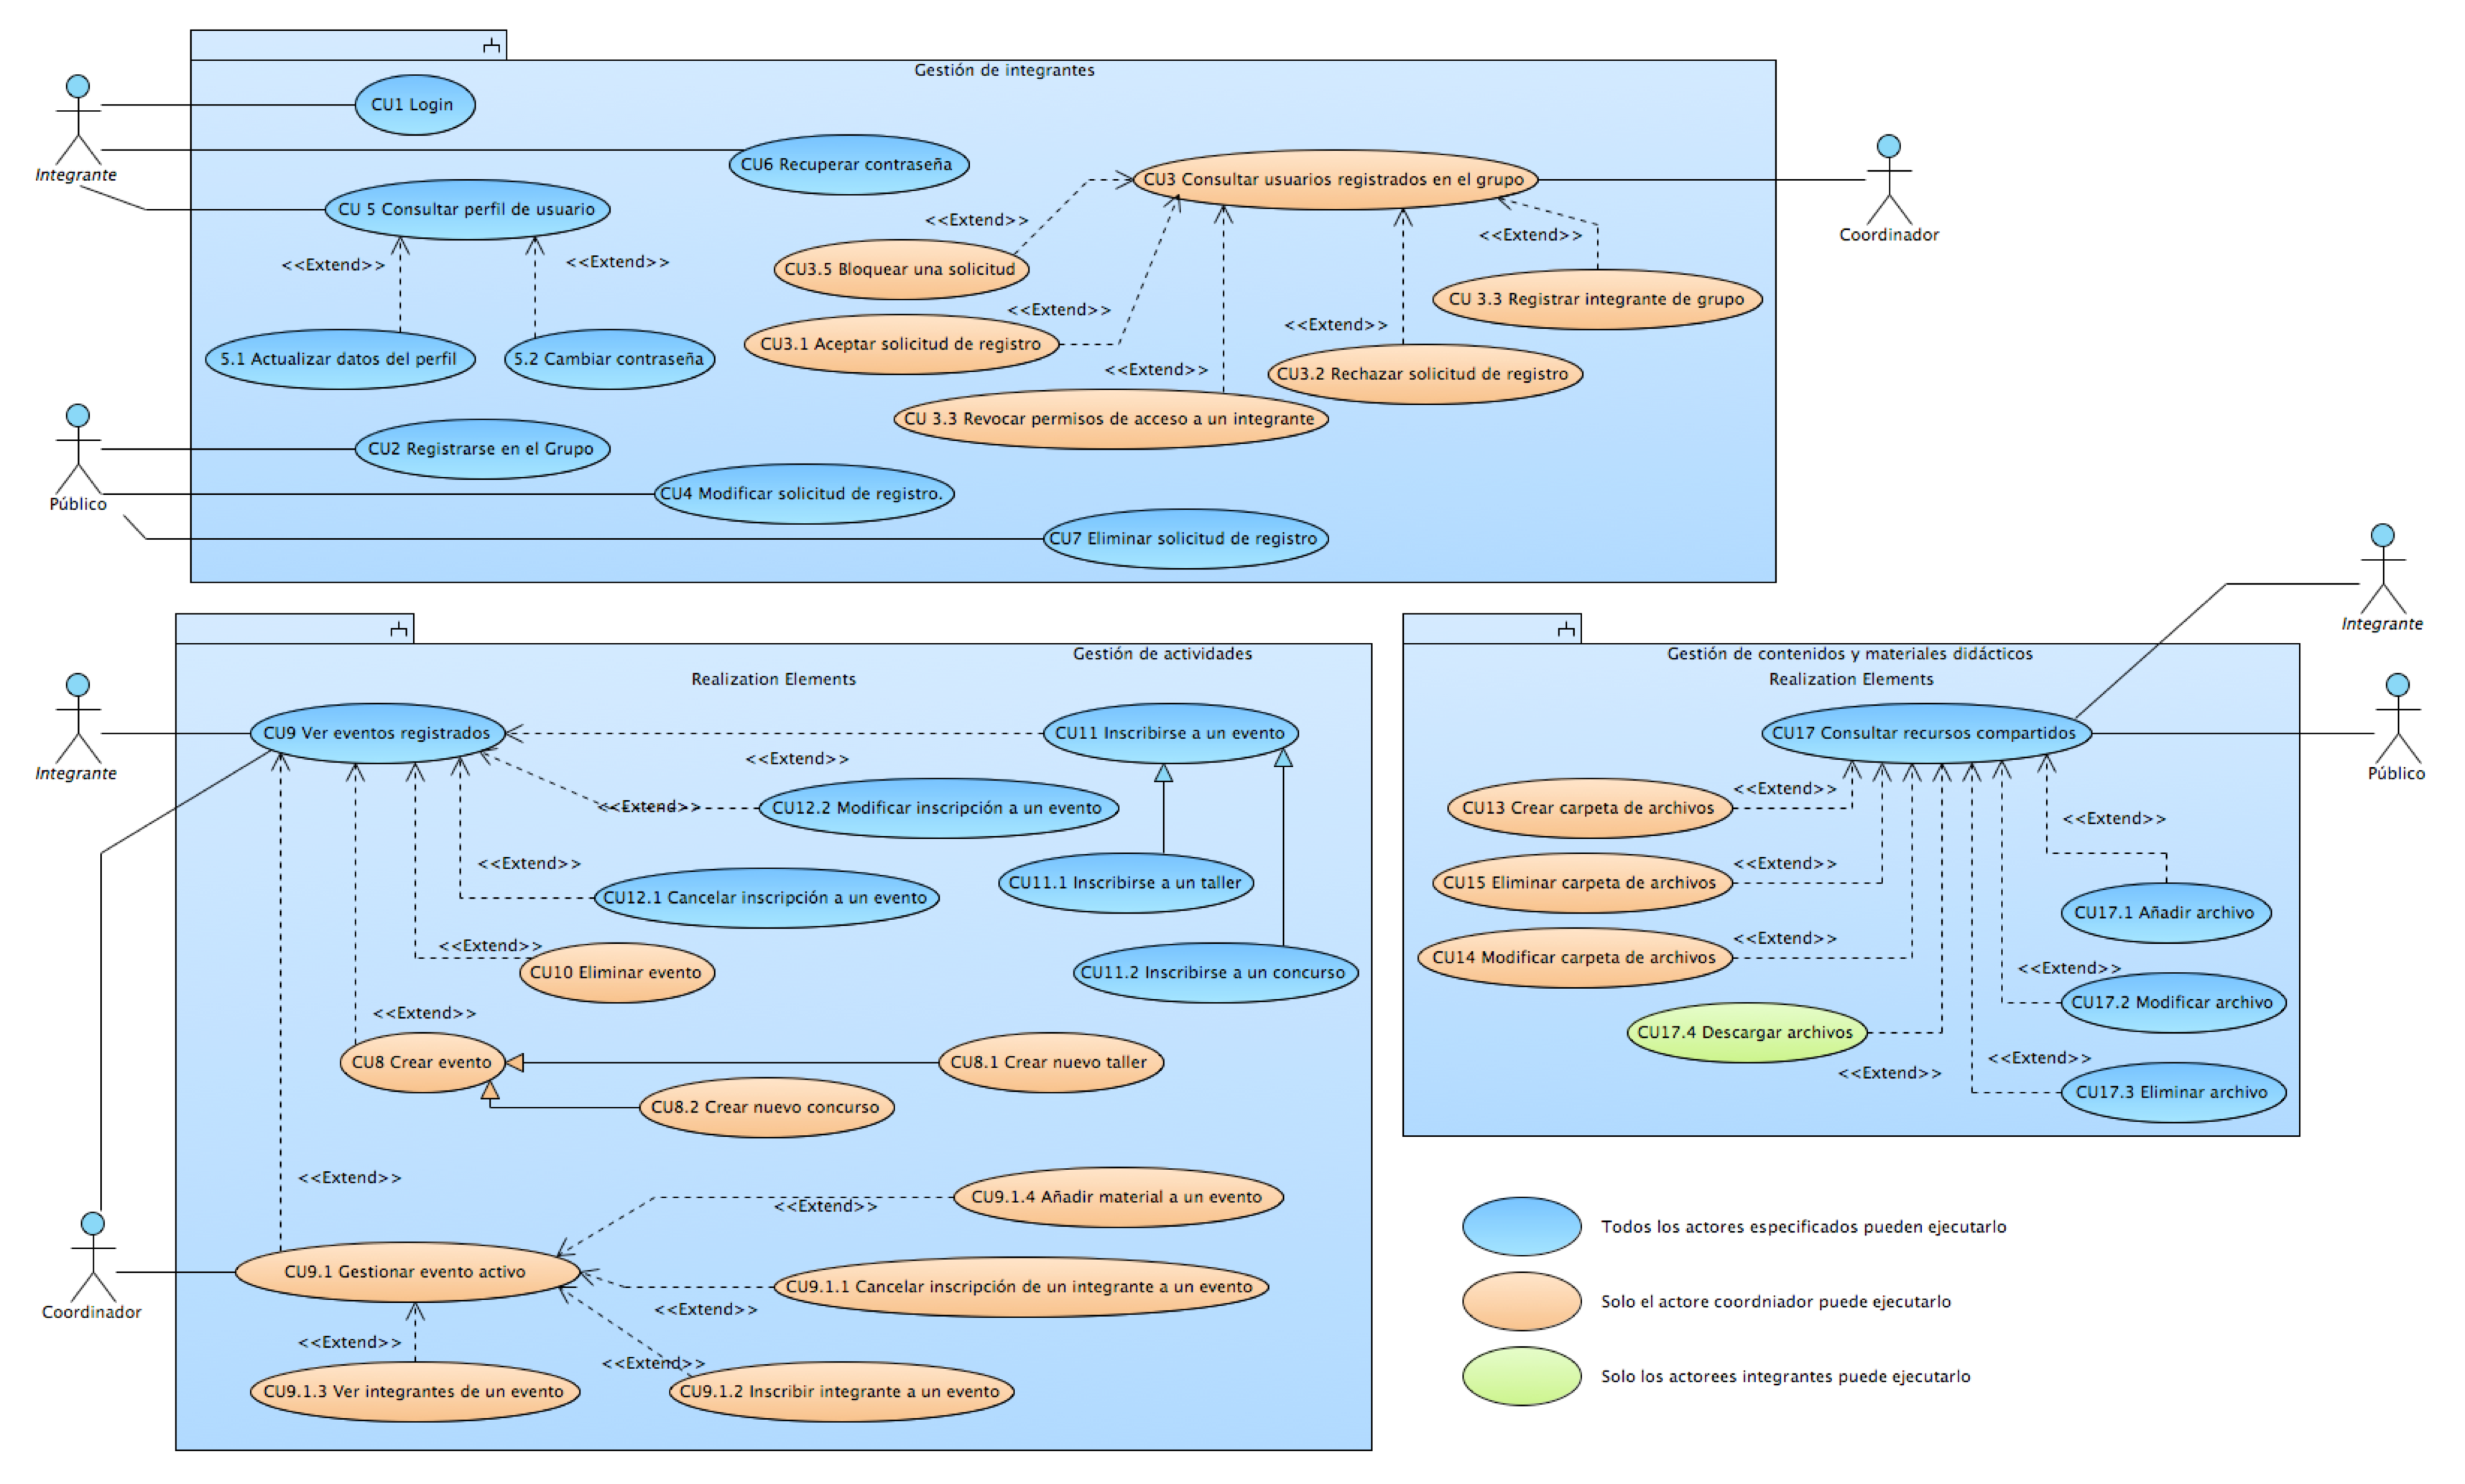
\includegraphics[angle=90, width=.7\textwidth]{images/casosDeUsoDetalle}
		\caption{Diagrama detallado del sistema.}
		\label{fig:casosDeUsoDetalle}
	\end{center}
\end{figure}

%---------------------------------------------------------
\section{Descripción de casos de uso}



A continuación se detallan los casos de uso.

%---------------------------------------------------------
% CASOS DE USO

%!TEX root = ../proyecto.tex

% Plantilla para caso de uso sencillo con ejemplos de comandos e intrucciones.
%-------------------------------------- COMIENZA descripción del caso de uso.

%\begin{UseCase}[archivo de imágen]{UCX}{Nombre del Caso de uso}{
%--------------------------------------
\begin{UseCase}{CU1}{Registrar Cliente}{
	Cuando un cliente quiere reservar en el hotel, se debe dar de alta en el sistema con sus datos personales, una vez registrado podrá ingresar al sistema.
}
	\UCitem{Versión}{\color{Gray}
		0.2	% Ponga un número de versión, 
	}\UCitem{Autor}{\color{Gray}
		Ruiz Evaristo Marco Antonio. % Analista responsable de especificar el CU
	}\UCitem{Supervisa}{\color{Gray}
		Hernández Jiménez Erick Yael. % Analista responsable de verificar que está correcto.
	% TODO: Dar de alta al actor Usuario
	}\UCitem{Actor}{
		\hyperlink{Cliente}{Cliente} % No olvide dar de alta el actor.
	}\UCitem{Propósito}{\begin{Titemize}%Indique los fines, objetivos, propósitos o valores agregados del Caso de uso.
		\Titem Permitir al cliente realizar reservaciones y registrar mascotas.
		\Titem Garantizar la privacidad de los datos del cliente y soportar la responsabilidad de los clientes en el sistema.
	\end{Titemize}
	}\UCitem{Entradas}{\begin{Titemize}
		% TODO: Dar de alta las entidades que se listan.
		\Titem \hyperlink{Cliente.nombre}{Nombre(s)} del cliente % El identificador no acepta acentos, espacios ni eñes.
		\Titem \hyperlink{Cliente.primerApellido}{Primer apellido} del cliente % Liste todos los datos de entrada
		\Titem \hyperlink{Cliente.segundoApellido}{Segundo apellido} del cliente. 
		\Titem \hyperlink{Cliente.CURP}{CURP } del cliente
		\Titem \hyperlink{Cliente.telefono}{Numero telefonico} del cliente.
		\Titem \hyperlink{Cliente.correo}{Correo electónico} del cliente
		\Titem \hyperlink{Cliente.direccion}{Ubicación origen} coordenadas latitud y longitud.
		\Titem \hyperlink{Cliente.Atributo}{Contraseña} con confirmación.
		\end{Titemize}
	}\UCitem{Origen}{\begin{Titemize}
		\Titem Se introducen desde el teclado y mouse.
		\Titem Ubicacion origen. La selecciona el usuario en el mapa % Indique por que medio se introducen los datos, 
	\end{Titemize}
	}\UCitem{Salidas}{\begin{Titemize}
		% TODO: Dar de alta las entidades que se listan.
		\Titem Mensajes de error. %Agregar errores explícitamente
		
	\end{Titemize}
	}\UCitem{Destino}{\begin{Titemize}
%		\Titem Se muestra en la pantalla \IUref{IU01}{}.. % Indique por que medio se muestran los datos, 
%		\Titem otros.          % Si es ḿas de uno indique que datos corresponden en cada medio de entrada.
		\Titem Se muestra en la pantalla \IUref{IU1}{Registrar cliente}.
	\end{Titemize}
	}\UCitem{Precondiciones}{\begin{Titemize}
		\Titem No debe haber otro cliente registrado con el mismo CURP ni correo electrónico.
	\end{Titemize}
	}\UCitem{Postcondiciones}{\begin{Titemize}
		\Titem Habrá un nuevo cliente registrado en el sistema.
		\Titem El cliente podrá registrar mascotas.
		\Titem El cliente podrá realizar reservaciones.
		\Titem El cliente podrá iniciar sesión.
		\Titem Se mostrara la pantalla \IUref{IU5}{Home cliente}
	\end{Titemize}
	}\UCitem{Errores}{\begin{Titemize}
		% Escriba todos los errores que puedan ocurrir en el sistema, para cada error recuerde:
		% Punerle un identificador
		% Describir la condición o escenario que detona el error
		% Describa la forma en que debe reaccionar el sitema: si la reaccion corresponde a varios pasos use mejor una trayectoria alternativa.
		% Relacione el error con la trayectoria principal.
		\Titem {\bf \hypertarget{CU1.E1}{E1}}: Cuando el cliente no haya llenado algun campo obligatorio, el sistema muestra el mensaje \MSGref{MSG-001}{Campo obligatorio} y regresa al paso \ref{UC1.paso3}.
			\Titem {\bf \hypertarget{CU1.E2}{E2}}: Cuando el CURP del cliente ya este registrado en el sistema, el sistema muestra el mensaje \MSGref{MSG-005}{CURP ya existente} y regresa al paso \ref{UC1.paso3}.
			\Titem {\bf \hypertarget{CU1.E3}{E3}}: Cuando el correo electronico del cliente ya este registrado en el sistema, el sistema muestra el mensaje \MSGref{MSG-006}{Correo electrónico ya existente} y regresa al paso \ref{UC1.paso3}
			\Titem {\bf \hypertarget{CU1.E4}{E4}}: Cuando el cliente ingrese un tipo de dato diferente al solicitado, el sistema muestra el mensaje \MSGref{MSG-007}{Dato no válido} y regresa al paso \ref{UC1.paso3}
			
	\end{Titemize}
	}\UCitem{Tipo}{
		% Especifique el tipo de caso de us, puede ser: "Caso de uso primario" o 
		% "Viene de \\hyperref{CUY}{CUY nombre del CU}" cuando se desprende desde otro caso de uso mediante un extends.
		Caso de uso primario
	}\UCitem{Observaciones}{
		% Indique las observaciones al caso de uso, las cuales pueden ser:
		%
		 Ninguna
		% - Dudas sobre el procedimiento o la especificación.
		% - Issues detectados
		% - Suposiciones realizadas.
		% - Cualquier otra especificacion que considere pertinente que no pudo colocarse en los demás atributos del Caso de uso
		% - Aclaraciones.
		% - Notas para el usuario o desarrollador.
		% - Pendientes (TODO's) en caso de no usar los comentarios.
	}
\end{UseCase}

%--------------------------------------
\begin{UCtrayectoria}
	% Cada paso debe inicair con un Verbo en infinitivo, siempre especificando el objetivo del paso mas la accion en concreto.
	% \UCpaso[\UCactor] se refiere al actor y \UCpaso se refiere al sistema.
	% A continuación viene ejemplos de pasos:
	% En el siguiente paso: "Ingresa al sistema" es el objetivo del paso y "escribiendo la URL de la aplicación" es la acción en concreto.
	\UCpaso[] \label{UC1.paso1}El cliente indica al sistema que desea registrarse presionando el botón \IUbutton{Registrar cliente} de la pantalla \IUref{IU3}{Pantalla de inicio}.
    \UCpaso[] \label{UC1.paso2}El sistema solicita los datos personales del cliente mediante la pantalla \IUref{IU1}{Registrar Cliente}.
    \UCpaso[] \label{UC1.paso3} El cliente proporciona sus datos personales.
    \UCpaso[] \label{UC1.paso4} El cliente solicita el registro mediante el botón \IUbutton{Registrar} de la pantalla \IUref{IU2}{Registrar Cliente}.
    \UCpaso[] El sistema verifica que todos los campos obligatorios se hayan llenado \ErrorRef{CU1}{E1}{Campo obligatorio}.
    \UCpaso[] El sistema verifica que los datos introducidos tengan un formato válido en los campos correspondientes \ErrorRef{CU1}{E4}{Dato no válido}.
    \UCpaso[] \label{UC1.paso5} El sistema verifica que no haya un cliente ya registrado con el mismo CURP \ErrorRef{CU1}{E2}{CURP ya existente}.
    \UCpaso[] \label{UC1.paso6} El sistema verifica que no haya un cliente ya registrado con el mismo correo electrónico \ErrorRef{CU1}{E3}{Correo electrónico ya existente}.
    \UCpaso[] \label{UC1.paso7} El sistema muestra la pantalla \IUref{IU5}{Home cliente} con el mensaje \MSGref{MSG-003}{No hay reservaciones}.
\end{UCtrayectoria}


%--------------------------------------
% Las trayectorias alternativas se identifican con Letras: A, B, C, etc.


%--------------------------------------
% Puntos de extensión

% Comente la siguiente sección en caso de que no hayan puntos de extensión o relaciones de tipo extends.
%\subsection{Puntos de extensión}
%\UCExtenssionPoint{
	% Cuando se dá la extensión del Caso de uso:
%	El usuario no recuerda cual es su contraseña o sospecha que su usuario está bloqueado.
%}{
	% Durante la región (en que pasos se puede dar la extensión):
%	Del paso \ref{CUX.etiqueta} al paso \ref{CUX.etiqueta}.
%}{
	% Casos de uso a los que extiende:
%	\UCref{CUZ}{Nombre del caso de uso}.
%}
		
		
		
%-------------------------------------- TERMINA descripción del caso de uso.
%!TEX root = ../proyecto.tex

% Plantilla para caso de uso sencillo con ejemplos de comandos e intrucciones.
%-------------------------------------- COMIENZA descripción del caso de uso.

%\begin{UseCase}[archivo de imágen]{UCX}{Nombre del Caso de uso}{
%--------------------------------------
\begin{UseCase}{CU2}{Registrar Reservación}{
		Cuando un cliente quiere realizar una reservación en hotel, debe registrar sus datos de reservación, una vez registrados se creara la reservación y se mostraran los detalles de la misma.
	}
	\UCitem{Versión}{\color{Gray}
		0.3	% Ponga un número de versión, 
	}\UCitem{Autor}{\color{Gray}
		Hernández Jiménez Erick Yael. % Analista responsable de especificar el CU
	}\UCitem{Supervisa}{\color{Gray}
		Ruiz Evaristo Marco Antonio. % Analista responsable de verificar que está correcto.
		% TODO: Dar de alta al actor Usuario
	}\UCitem{Actor}{
		\hyperlink{Cliente}{Cliente}% No olvide dar de alta el actor.
	}\UCitem{Propósito}{\begin{Titemize}%Indique los fines, objetivos, propósitos o valores agregados del Caso de uso.
		\Titem Proporcionar a los clientes un medio conveniente para realizar reservaciones para sus mascotas, permitiendo planificar sus necesidades de cuidado con anticipación.
		\Titem Gestionar la disponibilidad de las reservaciones, evitando conflictos y asegurando que los recursos estén bien distribuidos.
		\Titem Asegurar que todos los datos relevantes se ingresen de manera correcta y completa para el uso efectivo de los servicios.
		\Titem Ofrecer un medio para enviar recordatorios al cliente sobre las reservas próximas, reduciendo así el riesgo de cancelaciones tardías o ausencias.
		\end{Titemize}
	}\UCitem{Entradas}{\begin{Titemize}
			\Titem \hyperlink{SUCURSAL.NOMBRE_SUCURSAL}{Sucursal}.
			\Titem \hyperlink{DISPONIBILIDAD.CHECK-IN}{Check-in}
			\Titem \hyperlink{DISPONIBILIDAD.CHECK-OUT}{Check-out}.
			\Titem \hyperlink{ESPECIE.NOMBRE_ESPECIE}{Especies} de las mascotas a hospedar.
			\Titem \hyperlink{RAZA.NOMBRE_RAZA}{Razas} de las mascotas a hospedar.
			\Titem Número de mascotas de la misma raza que el cliente desea hospedar.
			\Titem \hyperlink{TAMANO.TAMANO}{Tamaños} de las mascotas a hospedar.
			\Titem \hyperlink{TIPO_CUARTO.NOMBRE_CUARTO}{Nombre de los cuartos} que desea reservar el cliente.
			\Titem \hyperlink{TIPO_SERVICIO.NOMBRE_SERVICIO}{Nombre de los servicios} que desea adquirir para la mascota el cliente.
		\end{Titemize}
	}\UCitem{Origen}{\begin{Titemize}
			\Titem \hyperlink{SUCURSAL.NOMBRE_SUCURSAL}{Sucursal}: Menú desplegable en la pantalla \IUref{IU6}{Búsqueda de hospedajes}.
			\Titem \hyperlink{DISPONIBILIDAD.CHECK-IN}{Check-in}: Selector de fechas en la pantalla \IUref{IU6}{Búsqueda de hospedajes}.
			\Titem \hyperlink{DISPONIBILIDAD.CHECK-OUT}{check-out}: Selector de fechas en la pantalla \IUref{IU6}{Búsqueda de hospedajes}.
			\Titem \hyperlink{ESPECIE.NOMBRE_ESPECIE}{Especies}: Menú desplegable en la pantalla \IUref{IU6}{Búsqueda de hospedajes}.
			\Titem \hyperlink{RAZA.NOMBRE_RAZA}{Razas}: Menú desplegable en la pantalla \IUref{IU6}{Búsqueda de hospedajes}.
			\Titem \hyperlink{TAMANO.TAMANO}{Tamaños}: Menú desplegable en la pantalla \IUref{IU6}{Búsqueda de hospedajes}.
			\Titem \hyperlink{TIPO_CUARTO.NOMBRE_CUARTO}{Nombre de los cuartos}: Botones de selección en la pantalla \IUref{IU7}{Catálogo de habitaciones}.
			\Titem \hyperlink{TIPO_SERVICIO.NOMBRE_SERVICIO}{Nombre de servicios}: Menú desplegable en la pantalla \IUref{IU9}{Servicios adicionales}.
		\end{Titemize}
	}\UCitem{Salidas}{\begin{Titemize}
			\Titem \hyperlink{SUCURSAL.NOMBRE_SUCURSAL}{Sucursal}.
			\Titem \hyperlink{DISPONIBILIDAD.CHECK-IN}{Check-in}.
			\Titem \hyperlink{DISPONIBILIDAD.CHECK-OUT}{Check-out}.
			\Titem \hyperlink{ESPECIE.NOMBRE_ESPECIE}{Especies} de las mascotas a hospedar.
			\Titem \hyperlink{RAZA.NOMBRE_RAZA}{Razas} de las mascotas a hospedar.
			\Titem \hyperlink{TAMANO.TAMANO}{Tamaños} de las mascotas a hospedar.
			\Titem \hyperlink{TIPO_CUARTO.NOMBRE_CUARTO}{Nombre de los cuartos} que desea reservar el cliente.
			\Titem \hyperlink{TIPO_CUARTO.PRECIO_CUARTO}{Precio del los cuartos} que desea reservar el cliente.
			\Titem \hyperlink{SUCURSAL.CALLE_DIRECCION}{Calle} de la sucursal en la que reserva el cliente.
			\Titem \hyperlink{SUCURSAL.NUMERO_DIRECCION}{Número de calle} de la sucursal en la que reserva el cliente.
			\Titem \hyperlink{SUCURSAL.NOMBRE_COLONIA_DIRECCION}{Colonia} de la sucursal en la que reserva el cliente.
			\Titem \hyperlink{SUCURSAL.NOMBRE_MUNICIPIO_DIRECCION}{Municipio} de la sucursal en la que reserva el cliente.
			\Titem \hyperlink{SUCURSAL.CODIGO_POSTAL_DIRECCION}{Código postal} de la sucursal en la que reserva el cliente.
			\Titem \hyperlink{SUCURSAL.ENTIDAD_DIRECCION}{Entidad} de la sucursal en la que reserva el cliente.
			\Titem \hyperlink{TIPO_SERVICIO.NOMBRE_SERVICIO}{Nombre de los servicios} que desea adquirir para la mascota el cliente.
			\Titem \hyperlink{TIPO_SERVICIO.COSTO_BASE}{Costo base de los servicios} que desea adquirir para la mascota el cliente.
			\Titem \hyperlink{TIPO_SERVICIO.COSTO_EXTRA}{Costo extra de los servicios} que desea adquirir para la mascota el cliente en caso de presentarse la necesidad de servicios emergentes.
			\Titem \hyperlink{CORTE_RESERVACION.SUMA_PRECIO_CUARTOS}{Total de los cuartos} que contrata el cliente.
			\Titem \hyperlink{CORTE_RESERVACION.SUMA_PRECIO_CITAS_SERVICIOS}{Total de los servicios} que contrata el cliente.
			\Titem \hyperlink{CORTE_RESERVACION.SUMA_TOTAL_RESERVACION}{Suma total por el hospedaje} que contrata el cliente.
		\end{Titemize}
	}\UCitem{Destino}{\begin{Titemize}
			\Titem \hyperlink{SUCURSAL.NOMBRE_SUCURSAL}{Sucursal}: En la pantalla  \IUref{IU7}{Catálogo de habitaciones} y \IUref{IU8}{Vista general del cuarto}.
			\Titem \hyperlink{DISPONIBILIDAD.CHECK-IN}{Check-in}: En la pantalla \IUref{IU7}{Catálogo de habitaciones} y \IUref{IU8}{Vista general del cuarto}.
			\Titem \hyperlink{DISPONIBILIDAD.CHECK-OUT}{check-out}: En la pantalla \IUref{IU7}{Catálogo de habitaciones} y \IUref{IU8}{Vista general del cuarto}.
			\Titem \hyperlink{ESPECIE.NOMBRE_ESPECIE}{Especies}: En la pantalla \IUref{IU7}{Catálogo de habitaciones} y \IUref{IU8}{Vista general del cuarto}.
			\Titem \hyperlink{RAZA.NOMBRE_RAZA}{Razas}: En la pantalla \IUref{IU7}{Catálogo de habitaciones} y \IUref{IU8}{Vista general del cuarto}.
			\Titem \hyperlink{TAMANO.TAMANO}{Tamaños}: En la pantalla \IUref{IU7}{Catálogo de habitaciones} y \IUref{IU8}{Vista general del cuarto}.
			\Titem \hyperlink{TIPO_CUARTO.NOMBRE_CUARTO}{Nombre de los cuartos}: En la pantalla \IUref{IU7}{Catálogo de habitaciones} y \IUref{IU8}{Vista general del cuarto}.
			\Titem \hyperlink{TIPO_CUARTO.PRECIO_CUARTO}{Precio de los cuartos}: En la pantalla \IUref{IU7}{Catálogo de habitaciones} y \IUref{IU8}{Vista general del cuarto}.
			\Titem \hyperlink{SUCURSAL.CALLE_DIRECCION}{Calle}: En un mapa en la pantalla \IUref{IU8}{Vista general del cuarto}.
			\Titem \hyperlink{SUCURSAL.NUMERO_DIRECCION}{Número de calle}: En un mapa en la pantalla \IUref{IU8}{Vista general del cuarto}.
			\Titem \hyperlink{SUCURSAL.NOMBRE_COLONIA_DIRECCION}{Colonia}: En un mapa en la pantalla \IUref{IU8}{Vista general del cuarto}.
			\Titem \hyperlink{SUCURSAL.NOMBRE_MUNICIPIO_DIRECCION}{Municipio}: En un mapa en la pantalla \IUref{IU8}{Vista general del cuarto}.
			\Titem \hyperlink{SUCURSAL.CODIGO_POSTAL_DIRECCION}{Código postal}: En un mapa en la pantalla \IUref{IU8}{Vista general del cuarto}.
			\Titem \hyperlink{SUCURSAL.ENTIDAD_DIRECCION}{Entidad}: En un mapa en la pantalla \IUref{IU8}{Vista general del cuarto}.
			\Titem \hyperlink{TIPO_SERVICIO.NOMBRE_SERVICIO}{Nombre de los servicios}: En la pantalla \IUref{IU9}{Servicios adicionales}.
			\Titem \hyperlink{TIPO_SERVICIO.COSTO_BASE}{Costo base de los servicios}: En la pantalla \IUref{IU9}{Servicios adicionales}.
			\Titem \hyperlink{TIPO_SERVICIO.COSTO_EXTRA}{Costo extra de los servicios}: En la pantalla \IUref{IU9}{Servicios adicionales}.
			\Titem \hyperlink{CORTE_RESERVACION.SUMA_PRECIO_CUARTOS}{Total de los cuartos}: En la pantalla \IUref{IU9}{Servicios adicionales} y en la pantalla \IUref{IU11}{Resumen del hospedaje}.
			\Titem \hyperlink{CORTE_RESERVACION.SUMA_PRECIO_CITAS_SERVICIOS}{Total de los servicios}: En la pantalla \IUref{IU9}{Servicios adicionales} y en la pantalla \IUref{IU11}{Resumen del hospedaje}.
			\Titem \hyperlink{CORTE_RESERVACION.SUMA_TOTAL_RESERVACION}{Suma total por el hospedaje}: En la pantalla \IUref{IU9}{Servicios adicionales} y en la pantalla \IUref{IU11}{Resumen del hospedaje}.
		\end{Titemize}
	}\UCitem{Precondiciones}{\begin{Titemize}
			% Incluya Precondiciones lógicas, de negocio e incluso las que debe atender el usuario. 
			\Titem Debe haber al menos un cuarto en al menos una sucursal.
			\Titem El cliente debe acceder al sistema por el caso de uso \UCref{CUX}{Iniciar Sesion} o \UCref{CU1}{Registrar Cliente}.
			\Titem Debe haber disponibilidad de habitaciones en las fechas deseadas.
		\end{Titemize}
	}\UCitem{Postcondiciones}{\begin{Titemize}
			\Titem Habrá una nueva reservación registrada para este cliente en el sistema.
			\Titem El calendario de disponibilidad se ha actualizado para reflejar las fechas reservadas.
			\Titem El cliente ha recibido una confirmación de la reservación a traves de la pantalla \IUref{IU5}{Home Cliente} y de un correo electrónico.
			\Titem Se habilitará el botón \IUbutton{Mascotas} en la pantalla \IUref{IU5}{Home Cliente}
			\Titem Todas las mascotas que el cliente haya asociado a la reservación serán accesibles para el cliente en la pantalla \IUref{IUX}{Consultar mascotas propias}.
		\end{Titemize}
	}\UCitem{Errores}{\begin{Titemize}
			\Titem {\bf \hypertarget{CU2.E1}{E1}}: Cuando el cliente no haya iniciado sesión en el sistema, se le indica que es \MSGref{MSG-013}{Necesario iniciar sesión} y dirige al cliente al caso de uso \IUref{CU1}.
			\Titem {\bf \hypertarget{CU2.E2}{E2}}: Cuando el cliente no haya ingresado los datos mínimos necesarios para la operación, se le muestra el mensaje  \MSGref{MSG-001}{Campo obligatorio} y regresa al paso anterior.
			\Titem {\bf \hypertarget{CU2.E3}{E3}}: Cuando el cliente ingrese un tipo de dato diferente al solicitado, el sistema muestra el mensaje \MSGref{MSG-007}{Dato no válido} y regresa dos pasos antes.
			\Titem {\bf \hypertarget{CU2.E4}{E4}}: Cuando no haya cuartos en el periodo indicado con las características que el cliente solicita, el sistema muestra el mensaje \MSGref{MSG-008}{Fecha no disponible} y dirige al cliente a la pantalla \IUref{IU6}{Búsqueda de hospedajes}.
			\Titem {\bf \hypertarget{CU2.E5}{E5}}: Cuando el cliente solicite la información de un cuarto al que no se puede acceder, el sistema muestra el mensaje \MSGref{MSG-014}{Detalles del cuarto no disponibles} y actualiza la pantalla \IUref{IU7}{Catálogo de habitaciones}.
			\Titem {\bf \hypertarget{CU2.E6}{E6}}: Cuando no haya disponibilidad de servicios extra en el periodo indicado con las características que el cliente solicita, el sistema muestra el mensaje \MSGref{MSG-015}{Servicios no disponibles}.
		\end{Titemize}
	}\UCitem{Tipo}{
		Caso de uso primario
	}\UCitem{Observaciones}{
		Se considera que la disponibilidad de habitaciones y servicios no cambia durante la realización del registro de reservación.
	}
\end{UseCase}

%--------------------------------------
\begin{UCtrayectoria}
	\UCpaso[] El cliente selecciona  el botón \IUbutton{Realizar reservación} de la pantalla \IUref{IU5}{Home Cliente}.
	\UCpaso[] El sistema verifica que el cliente ya se encuentre ingresado en el sistema con un perfil de usuario \ErrorRef{CU2}{E1}{Necesario iniciar sesión}.
	\UCpaso[] El sistema solicita los datos para buscar cuartos que sean de interés para cliente mediante la pantalla \IUref{IU6}{Búsqueda de hospedajes}.
	\UCpaso[] El cliente introduce los datos para buscar cuartos en la sucursal de su preferencia y selecciona el botón \IUbutton{Buscar}.
	\UCpaso[] El sistema verifica que se hayan introducido todos los datos necesarios para la búsqueda \ErrorRef{CU2}{E2}{Campo obligatorio}.
	\UCpaso[] El sistema verifica que se hayan introducido datos válidos para la búsqueda \ErrorRef{CU2}{E3}{Dato no válido}.
	\UCpaso[] El sistema verifica que se haya cuartos disponibles en el periodo y con todas las características solicitadas \ErrorRef{CU2}{E4}{Fecha no disponible}.
	\UCpaso[] \label{muestra_catalogo}El sistema muestra todos los cuartos que cumplan con los requisitos deseados, mostrando el mensaje \MSGref{MSG-016}{Cuartos para mascotas} en la pantalla \IUref{IU7}{Catálogo de habitaciones}.
	\UCpaso[] El cliente selecciona el botón \IUbutton{Seleccionar} correspondiente al cuarto de interés en la pantalla \IUref{IU7}{Catálogo de habitaciones}.
	\UCpaso[] El sistema verifica que se puedan acceder a los datos del cuarto de interés \ErrorRef{CU2}{E5}{Detalles de cuarto no disponibles} y dirige al cliente a la pantalla \IUref{IU8}{Vista general del cuarto}.
	\UCpaso[] El cliente ingresa el número de mascotas de la misma raza y tamaño que desea asociar al mismo cuarto.
	\UCpaso[] El sistema verifica que se hayan introducido todos los datos necesarios para la reservación \ErrorRef{CU2}{E2}{Campo obligatorio}.
	\UCpaso[] El sistema verifica que se hayan introducido datos válidos para la reservación\ErrorRef{CU2}{E3}{Dato no válido}.
	\UCpaso[] Se repite desde el paso \hyperlink{muestra_catalogo}{7} hasta haber reservado para todas las mascotas que haya introducido el cliente inicialmente.
	\UCpaso[] El sistema dirige al cliente a la pantalla \IUref{IU9}{Servicios adicionales} con los campos necesarios para agregar cita a tantas mascotas como haya indicado inicialmente y desee mientras haya servicios disponibles \ErrorRef{CU2}{E6}{Servicios no disponibles}.
	\UCpaso[] El cliente indica al sistema cuántos y qué servicios desea contratar, actualizando los costos totales en la pantalla tras cada modificación.
	\UCpaso[] El cliente indica al sistema que desea completar su reservación con el botón \IUbutton{Reservar}.
	\UCpaso[] \label{CU3_Reg_mascota}El sistema ofrece al cliente la posibilidad de dar más detalles de sus mascotas asociadas a la reservación \IUref{CU3}{Registrar Mascota} mediante la pantalla \IUref{IU10}{Registrar más detalles}.
	\UCpaso[] El sistema dirige al cliente a la pantalla de \IUref{IU11}{Resumen del hospedaje}.
	\UCpaso[] El cliente indica que desea proceder al pago con el botón \IUbutton{Pagar}.
	\UCpaso[] \label{CU2_Reg_pago}El sistema muestra la pantalla \IUref{IU5}{Registrar Pago}.
	\UCpaso[] El sistema registra la reservación y muestra la pantalla \IUref{IU5}{Home Cliente} con los detalles de la reservación.


	
\end{UCtrayectoria}


%--------------------------------------
% Las trayectorias alternativas se identifican con Letras: A, B, C, etc.

%--------------------------------------
% Puntos de extensión

% Comente la siguiente sección en caso de que no hayan puntos de extensión o relaciones de tipo extends.
\subsection{Puntos de extensión}
\UCExtenssionPoint{
	% Cuando se dá la extensión del Caso de uso:
	El cliente quiere agregar detalles de su mascota asociada a su reservación.
}{
	% Durante la región (en que pasos se puede dar la extensión):
	En el paso \ref{CU2_Reg_mascota}.
}{
	% Casos de uso a los que extiende:
	\UCref{CU3}{Resgistrar Mascota}.
}
\UCExtenssionPoint{
	% Cuando se dá la extensión del Caso de uso:
	El cliente quiere pagar  o consultar el costo de la reservación.
}{
	% Durante la región (en que pasos se puede dar la extensión):
	En el paso \ref{CU2_Reg_mascota}.
}{
	% Casos de uso a los que extiende:
	\UCref{CUZ}{Resgistrar Pago}.
}

%-------------------------------------- TERMINA descripción del caso de uso.
%!TEX root = ../proyecto.tex

% Plantilla para caso de uso sencillo con ejemplos de comandos e intrucciones.
%-------------------------------------- COMIENZA descripción del caso de uso.

%\begin{UseCase}[archivo de imágen]{UCX}{Nombre del Caso de uso}{
%--------------------------------------
\begin{UseCase}{CU3}{Registrar Mascota}{
		Cuando un cliente quiere realizar una reservacion en hotel, debe dar de alta en el sistema los datos de su mascota, una vez registrados continuara con la reservacion.
	}
	\UCitem{Versión}{\color{Gray}
		0.2	% Ponga un número de versión, 
	}\UCitem{Autor}{\color{Gray}
		Ruiz Evaristo Marco Antonio. % Analista responsable de especificar el CU
	}\UCitem{Supervisa}{\color{Gray}
		Hernández Jiménez Erick Yael. % Analista responsable de verificar que está correcto.
		% TODO: Dar de alta al actor Usuario
	}\UCitem{Actor}{
		\hyperlink{Cliente}{Cliente}% No olvide dar de alta el actor.
	}\UCitem{Propósito}{\begin{Titemize}%Indique los fines, objetivos, propósitos o valores agregados del Caso de uso.
		\Titem Facilitar al cliente la reservación de manera eficiente, ofreciendo un proceso intuitivo y simplificado para satisfacer sus necesidades.
		\Titem Garantizar la seguridad y privacidad de los datos de las mascotas, además de proporcionar un sistema confiable que soporte las necesidades de los clientes al manejar eficientemente sus requerimientos.
		\Titem Almacenar los datos de las mascotas de forma segura para permitir reservaciones futuras, mejorando la experiencia del cliente al proporcionar un proceso de reservación más rápido y personalizado.
		\end{Titemize}
	}\UCitem{Entradas}{\begin{Titemize}
			% TODO: Dar de alta las entidades que se listan.
			\Titem \hyperlink{mascota.nombre}{Nombre}. % El identificador no acepta acentos, espacios ni eñes.
			\Titem \hyperlink{mascota.tamano}{Tamaño}. % Liste todos los datos de entrada
			\Titem \hyperlink{mascota.fechaNacimiento}{Fecha de nacimiento}. 
			\Titem \hyperlink{mascota.RUAC}{RUAC}.
			\Titem \hyperlink{mascota.especie}{Especie}.
			\Titem \hyperlink{mascota.raza}{Raza}.
			\Titem \hyperlink{mascota.color}{Color}.
			\Titem \hyperlink{mascota.vacunasAplicadas}{Vacunas aplicadas}.
			\Titem \hyperlink{mascota.alergias}{Alergias}.
			\Titem \hyperlink{mascota.medicamentos}{Medicamentos}
			\Titem \hyperlink{mascota.comentariosExtra}{Comentarios extra}.
		\end{Titemize}
	}\UCitem{Origen}{\begin{Titemize}
			\Titem Se introducen desde el teclado. % Indique por que medio se introducen los datos, 
			\Titem Se seleccionan de un selector de fecha (calendario) con el mouse.
			\Titem Se marca un checkbox con el mouse.
		
		\end{Titemize}
	}\UCitem{Salidas}{\begin{Titemize}
			% TODO: Dar de alta las entidades que se listan.
			\Titem Mensajes de error. % Indique por que medio se introducen los datos, 
		\end{Titemize}
	}\UCitem{Destino}{\begin{Titemize}
			\Titem Se muestra en la pantalla \IUref{IU3}{Registrar Mascota}.
			\Titem Se muestra en la pantalla \IUref{IU2}{Registrar Reservacion}. 
			
		\end{Titemize}
	}\UCitem{Precondiciones}{\begin{Titemize}
			% Incluya Precondiciones lógicas, de negocio e incluso las que debe atender el usuario. 
			\Titem El cliente debe tener una cuenta	
			\Titem No debe haber otra mascota registrada con el mismo RUAC.
			\Titem La mascota debe contar con al menos las 3 vacunas solicitadas de acuerdo a \hyperlink{BR-002}{BR-002 Vacunas Obligatorias para la Mascota}
			% Muchas precondiciones provienen de reglas de negocios, otras estarán asociadas a manejo de errores
			% Otras están relacionadas con casos de uso que deben ejecutarse previamente, como registrar un producto.
		\end{Titemize}
	}\UCitem{Postcondiciones}{\begin{Titemize}
			\Titem Habrá una nueva mascota resgitrada para ese cliente en el sistema.
			\Titem La mascota aparecera en la lista de mascotas en la pantalla \IUref{IU5}{Regsitrar Reservacion}.
			\Titem El cliente podrá conservar los datos de la mascota registrada para reservaciones futuras.
			\Titem El cliente podrá realizar reservaciones.
			% Indique todas las postcondiciones
			% por ejemplo, Cambios en el sistema
			% Cambios en la BD una vez terminado el CU
			% Efectos colaterales
			% Condiciones de término.
		\end{Titemize}
	}\UCitem{Errores}{\begin{Titemize}
			% Escriba todos los errores que puedan ocurrir en el sistema, para cada error recuerde:
			% Punerle un identificador
			% Describir la condición o escenario que detona el error
			% Describa la forma en que debe reaccionar el sitema: si la reaccion corresponde a varios pasos use mejor una trayectoria alternativa.
			% Relacione el error con la trayectoria principal.
			\Titem {\bf \hypertarget{CU3.E1}{E1}}: Cuando el cliente no haya llenado algun campo obligatorio, el sistema muestra el mensaje \MSGref{MSG-001}{Campo obligatorio} y regresa al paso \ref{UC3.paso3}.
			\Titem {\bf \hypertarget{CU3.E2}{E2}}: Cuando el RUAC del cliente ya este registrado en el sistema, el sistema muestra el mensaje \MSGref{MSG-002}{RUAC ya existente} y regresa al paso \ref{UC3.paso3}.
.
			\Titem {\bf \hypertarget{CU3.E3}{E3}}: Cuando la mascota no cuenta con las 3 vacunas obligatorias, el sistema muestra el mensaje \MSGref{MSG-004}{Vacunas obligatorias} y regresa al paso \ref{UC3.paso3}
			\Titem {\bf \hypertarget{CU3.E4}{E4}}: Cuando el cliente ingrese un tipo de dato diferente al solicitado, el sistema muestra el mensaje \MSGref{MSG-007}{Dato no válido} y regresa al paso \ref{UC3.paso3}
			
		\end{Titemize}
	}\UCitem{Tipo}{
		% Especifique el tipo de caso de us, puede ser: "Caso de uso primario" o 
		% "Viene de \\hyperref{CUY}{CUY nombre del CU}" cuando se desprende desde otro caso de uso mediante un extends.
		Para ejecutar este caso de uso debe pasar primero por el \UCref{CUX}{Iniciar Sesion}. o \UCref{CU1}{Registrar Cliente} y estar en el caso de uso \UCref{CU2}{Regsitrar reservacion}
	}\UCitem{Observaciones}{
		% Indique las observaciones al caso de uso, las cuales pueden ser:
		Ninguna
		% - Dudas sobre el procedimiento o la especificación.
		% - Issues detectados
		% - Suposiciones realizadas.
		% - Cualquier otra especificacion que considere pertinente que no pudo colocarse en los demás atributos del Caso de uso
		% - Aclaraciones.
		% - Notas para el usuario o desarrollador.
		% - Pendientes (TODO's) en caso de no usar los comentarios.
	}
\end{UseCase}

%--------------------------------------
\begin{UCtrayectoria}
	% Cada paso debe inicair con un Verbo en infinitivo, siempre especificando el objetivo del paso mas la accion en concreto.
	% \UCpaso[\UCactor] se refiere al actor y \UCpaso se refiere al sistema.
	% A continuación viene ejemplos de pasos:
	% En el siguiente paso: "Ingresa al sistema" es el objetivo del paso y "escribiendo la URL de la aplicación" es la acción en concreto.
	\UCpaso[] \label{UC3.paso1} El cliente selecciona  el botón \IUbutton{Regsitrar nueva mascota} desde el formulario de la pantalla \IUref{IU2}{Registrar Reservacion}.
	\UCpaso [] \label{UC3.paso2} El sistema solicita los datos de la mascota mediante la pantalla  \IUref{IU3}{Registrar Mascota}.
	\UCpaso [] \label{UC3.paso3} El cliente proporciona los datos de su mascota.
	% En el siguiente paso está etiquetado para ser referenciado por un error o trayectoria alternativa:
	 \UCpaso[] \label{UC3.paso4} El cliente solicita el registro de la nueva mascota mediante el botón \IUbutton{Registrar} de la pantalla \IUref{IU2}{Registrar Mascota}.
	% En el siguiente paso se usa el comando \IUbutton 
\UCpaso[] {UC3.paso5}El sistema verifica que todos los campos obligatorios se hayan llenado \ErrorRef{CU3}{E1}{Campo obligatorio}.    \UCpaso[] {UC3.paso6} El sistema verifica que los datos introducidos tengan un formato válido en los campos correspondientes \ErrorRef{CU3}{E4}{Dato no válido}.
\UCpaso[] \label{UC3.paso7} El sistema verifica que no haya una mascota ya registrada con el mismo RUAC \ErrorRef{CU3}{E2}{RUAC ya existente}.
\UCpaso[] \label{UC3.paso8} El sistema verifica que la mascota cuente con las 3 vacunas obligatorias \ErrorRef{CU3}{E3}{Vacunas obligatoria}.
\UCpaso[] \label{UC3.paso9} El sistema registra la nueva mascota para ese cliente.
\UCpaso[] \label{UC3.paso10} El sistema muestra la pantalla \IUref{IU5}{Registar Reservacion} y la mascota esta disponible para ser seleccionada en la reservación.
	
\end{UCtrayectoria}


%--------------------------------------
% Las trayectorias alternativas se identifican con Letras: A, B, C, etc.

%--------------------------------------
% Puntos de extensión

% Comente la siguiente sección en caso de que no hayan puntos de extensión o relaciones de tipo extends.
\subsection{Puntos de extensión}
\UCExtenssionPoint{
	% Cuando se dá la extensión del Caso de uso:
El cliente quiere agregar un medicamento a su mascota.
}{
	% Durante la región (en que pasos se puede dar la extensión):
	Del paso \ref{UC3.paso3} al paso \ref{CUX.etiqueta}.
}{
	% Casos de uso a los que extiende:
	\UCref{CUZ}{Resgistrar Medicamento}.
}



%-------------------------------------- TERMINA descripción del caso de uso.
%!TEX root = ../proyecto.tex

% Plantilla para caso de uso sencillo con ejemplos de comandos e intrucciones.
%-------------------------------------- COMIENZA descripción del caso de uso.

%\begin{UseCase}[archivo de imágen]{UCX}{Nombre del Caso de uso}{
%--------------------------------------
\begin{UseCase}{CU4}{Eliminar reservacion}{
	Si el cliente tuvo algun inconveniente con su reservacion debe poder eliminar dicha reservacion, una vez eliminada se borran los datos de reservacion
}
	\UCitem{Versión}{\color{Gray}
		0.1	% Ponga un número de versión, 
	}\UCitem{Autor}{\color{Gray}
		Ruiz Evaristo Marco Antonio. % Analista responsable de especificar el CU
	}\UCitem{Supervisa}{\color{Gray}
		Hernández Jiménez Erick Yael. % Analista responsable de verificar que está correcto.
	% TODO: Dar de alta al actor Usuario
	}\UCitem{Actor}{
		\hyperlink{Cliente}{Cliente},
		\hyperlink{Recepcionista}{Recepsionista} % No olvide dar de alta el actor.
	}\UCitem{Propósito}{\begin{Titemize}%Indique los fines, objetivos, propósitos o valores agregados del Caso de uso.
		\Titem Controlar reservaciones.
	\end{Titemize}
	}\UCitem{Entradas}{\begin{Titemize}
		% TODO: Dar de alta las entidades que se listan.
		\Titem Ninguna
		\end{Titemize}
	}\UCitem{Origen}{\begin{Titemize}
		\Titem Se da click desde el mouse.          % Si es ḿas de uno indique que datos corresponden en cada medio de entrada
	\end{Titemize}
	}\UCitem{Salidas}{\begin{Titemize}
		% TODO: Dar de alta las entidades que se listan.
		\Titem Ninguna
	\end{Titemize}
	}\UCitem{Destino}{\begin{Titemize}
		\Titem Se muestra en la pantalla \IUref{IU3}{Pantalla de Home Cliente}
	\end{Titemize}
	}\UCitem{Precondiciones}{\begin{Titemize}
		% Incluya Precondiciones lógicas, de negocio e incluso las que debe atender el usuario. 
		% Muchas precondiciones provienen de reglas de negocios, otras estarán asociadas a manejo de errores
		% Otras están relacionadas con casos de uso que deben ejecutarse previamente, como registrar un producto.
		\Titem El cliente debe tener una cuenta
		\Titem El cliente debe tener una mascota registrada en una reservación.
	\end{Titemize}
	}\UCitem{Postcondiciones}{\begin{Titemize}
		% Indique todas las postcondiciones
		% por ejemplo, Cambios en el sistema
		% Cambios en la BD una vez terminado el CU
		% Efectos colaterales
		% Condiciones de término.
		\Titem Se eliminaran los datos de la mascota.
	\end{Titemize}
	}\UCitem{Errores}{\begin{Titemize}
		% Escriba todos los errores que puedan ocurrir en el sistema, para cada error recuerde:
		% Punerle un identificador
		% Describir la condición o escenario que detona el error
		% Describa la forma en que debe reaccionar el sitema: si la reaccion corresponde a varios pasos use mejor una trayectoria alternativa.
		% Relacione el error con la trayectoria principal.
		\Titem Ninguno
	\end{Titemize}
	}\UCitem{Tipo}{
		% Especifique el tipo de caso de us, puede ser: "Caso de uso primario" o 
		% "Viene de \\hyperref{CUY}{CUY nombre del CU}" cuando se desprende desde otro caso de uso mediante un extends.
		Para ejecutar este caso de uso debe pasar primero por el \UCref{CUX}{Iniciar Sesion}. o \UCref{CU1}{Registrar Cliente} y \UCref{CU2}{Registrar Mascota}
	}\UCitem{Observaciones}{
		% Indique las observaciones al caso de uso, las cuales pueden ser:
		 - Ninguna
		% - Dudas sobre el procedimiento o la especificación.
		% - Issues detectados
		% - Suposiciones realizadas.
		% - Cualquier otra especificacion que considere pertinente que no pudo colocarse en los demás atributos del Caso de uso
		% - Aclaraciones.
		% - Notas para el usuario o desarrollador.
		% - Pendientes (TODO's) en caso de no usar los comentarios.
	}
\end{UseCase}

%--------------------------------------
\begin{UCtrayectoria}
	% Cada paso debe inicair con un Verbo en infinitivo, siempre especificando el objetivo del paso mas la accion en concreto.
	% \UCpaso[\UCactor] se refiere al actor y \UCpaso se refiere al sistema.
	% A continuación viene ejemplos de pasos:
	% En el siguiente paso: "Ingresa al sistema" es el objetivo del paso y "escribiendo la URL de la aplicación" es la acción en concreto.
	\UCpaso[] El cliente indica al sistema que desea eliminar los datos de la reservacion haciendo click en el botón \IUbutton{Eliminar}. en la pantalla \IUref{UI5}{Pantalla de Home Cliente}.
	\UCpaso []El sistema elimina los datos de la reservacion. 
\end{UCtrayectoria}


%--------------------------------------
% Las trayectorias alternativas se identifican con Letras: A, B, C, etc.
%\begin{UCtrayectoriaA}{CUX}{LETRA}{Condición que hace que se ejecute esta trayectoria}
%	\UCpaso Especifique los pasos  de la trayectoria.
	% Se puede desprender otra trayectria alternativa si es necesario.
	% Finalice la trayectoria indicando si la ejecución se integra a la trayectoria anterior o si termina la ejecución del CU.
	% Verifique que la redacción de la trayectoria deje en claro si el objetivo del CU se alcanzó o no.
%	\UCpaso[] El Caso de Uso continúa en el paso \ref{UCX.introduceDatos}.
%\end{UCtrayectoriaA}


%--------------------------------------
% Puntos de extensión

% Comente la siguiente sección en caso de que no hayan puntos de extensión o relaciones de tipo extends.
%\subsection{Puntos de extensión}
%\UCExtenssionPoint{
	% Cuando se dá la extensión del Caso de uso:
%	El usuario no recuerda cual es su contraseña o sospecha que su usuario está bloqueado.
%}{
	% Durante la región (en que pasos se puede dar la extensión):
%	Del paso \ref{CUX.etiqueta} al paso \ref{CUX.etiqueta}.
%}{
	% Casos de uso a los que extiende:
%	\UCref{CUZ}{Nombre del caso de uso}.
%}
		
		
		
%-------------------------------------- TERMINA descripción del caso de uso.
%!TEX root = ../proyecto.tex

% Plantilla para caso de uso sencillo con ejemplos de comandos e intrucciones.
%-------------------------------------- COMIENZA descripción del caso de uso.

%\begin{UseCase}[archivo de imágen]{UCX}{Nombre del Caso de uso}{
%--------------------------------------
\begin{UseCase}{CU5}{Log-out}{
	Cuando un cliente a terminado de usar su sesion debe poder cerrar dicha sesion para que el cliente pueda mantener su sesion segura.
}
	\UCitem{Versión}{\color{Gray}
		0.1	% Ponga un número de versión, 
	}\UCitem{Autor}{\color{Gray}
		Ruiz Evaristo Marco Antonio. % Analista responsable de especificar el CU
	}\UCitem{Supervisa}{\color{Gray}
		Hernández Jiménez Erick Yael. % Analista responsable de verificar que está correcto.
	% TODO: Dar de alta al actor Usuario
	}\UCitem{Actor}{
		\hyperlink{Cliente}{Cliente},
		 % No olvide dar de alta el actor.
	}\UCitem{Propósito}{\begin{Titemize}%Indique los fines, objetivos, propósitos o valores agregados del Caso de uso.
		\Titem Proteger los datos del cliente.
		\Titem Mantener seguro el sistema.
	\end{Titemize}
	}\UCitem{Entradas}{\begin{Titemize}
		% TODO: Dar de alta las entidades que se listan.
		\Titem Ninguna
		\end{Titemize}
	}\UCitem{Origen}{\begin{Titemize}
		\Titem Se da click desde el mouse.     % Si es ḿas de uno indique que datos corresponden en cada medio de entrada.
	\end{Titemize}
	}\UCitem{Salidas}{\begin{Titemize}
		% TODO: Dar de alta las entidades que se listan.
		\Titem Ninguna
	\end{Titemize}
	}\UCitem{Destino}{\begin{Titemize}
		\Titem Se muestra en la pantalla \IUref{IU3}{Pantalla de Home Cliente}
	\end{Titemize}
	}\UCitem{Precondiciones}{\begin{Titemize}
		% Incluya Precondiciones lógicas, de negocio e incluso las que debe atender el usuario. 
		% Muchas precondiciones provienen de reglas de negocios, otras estarán asociadas a manejo de errores
		% Otras están relacionadas con casos de uso que deben ejecutarse previamente, como registrar un producto.
		\Titem El cliente debe tener una cuenta
	\end{Titemize}
	}\UCitem{Postcondiciones}{\begin{Titemize}
		% Indique todas las postcondiciones
		% por ejemplo, Cambios en el sistema
		% Cambios en la BD una vez terminado el CU
		% Efectos colaterales
		% Condiciones de término.
		\Titem Se cierra la sesion del cliente.
	\end{Titemize}
	}\UCitem{Errores}{\begin{Titemize}
		% Escriba todos los errores que puedan ocurrir en el sistema, para cada error recuerde:
		% Punerle un identificador
		% Describir la condición o escenario que detona el error
		% Describa la forma en que debe reaccionar el sitema: si la reaccion corresponde a varios pasos use mejor una trayectoria alternativa.
		% Relacione el error con la trayectoria principal.
		\Titem Ninguno
	\end{Titemize}
	}\UCitem{Tipo}{
		% Especifique el tipo de caso de us, puede ser: "Caso de uso primario" o 
		% "Viene de \\hyperref{CUY}{CUY nombre del CU}" cuando se desprende desde otro caso de uso mediante un extends.
		Para ejecutar este caso de uso debe pasar primero por el \UCref{CUX}{Iniciar Sesion}. o \UCref{CU1}{Registrar Cliente}
	}\UCitem{Observaciones}{
		% Indique las observaciones al caso de uso, las cuales pueden ser:
		% - Ninguna
		 Dudas sobre el procedimiento o la especificación.
		% - Issues detectados
		% - Suposiciones realizadas.
		- Falta definir los actores
		% - Aclaraciones.
		% - Notas para el usuario o desarrollador.
		% - Pendientes (TODO's) en caso de no usar los comentarios.
	}
\end{UseCase}

%--------------------------------------
\begin{UCtrayectoria}
	% Cada paso debe inicair con un Verbo en infinitivo, siempre especificando el objetivo del paso mas la accion en concreto.
	% \UCpaso[\UCactor] se refiere al actor y \UCpaso se refiere al sistema.
	% A continuación viene ejemplos de pasos:
	% En el siguiente paso: "Ingresa al sistema" es el objetivo del paso y "escribiendo la URL de la aplicación" es la acción en concreto.
	\UCpaso[] El cliente indica al sistema que desea cerrar sesion haciendo click en el botón \IUbutton{Salir}. en la pantalla \IUref{UI5}{Pantalla de Home Cliente}.
	\UCpaso []El sistema cierra la sesión. 
\end{UCtrayectoria}


%--------------------------------------
% Las trayectorias alternativas se identifican con Letras: A, B, C, etc.
%\begin{UCtrayectoriaA}{CUX}{LETRA}{Condición que hace que se ejecute esta trayectoria}
%	\UCpaso Especifique los pasos  de la trayectoria.
	% Se puede desprender otra trayectria alternativa si es necesario.
	% Finalice la trayectoria indicando si la ejecución se integra a la trayectoria anterior o si termina la ejecución del CU.
	% Verifique que la redacción de la trayectoria deje en claro si el objetivo del CU se alcanzó o no.
%	\UCpaso[] El Caso de Uso continúa en el paso \ref{UCX.introduceDatos}.
%\end{UCtrayectoriaA}


%--------------------------------------
% Puntos de extensión

% Comente la siguiente sección en caso de que no hayan puntos de extensión o relaciones de tipo extends.
%\subsection{Puntos de extensión}
%\UCExtenssionPoint{
	% Cuando se dá la extensión del Caso de uso:
%	El usuario no recuerda cual es su contraseña o sospecha que su usuario está bloqueado.
%}{
	% Durante la región (en que pasos se puede dar la extensión):
%	Del paso \ref{CUX.etiqueta} al paso \ref{CUX.etiqueta}.
%}{
	% Casos de uso a los que extiende:
	%\UCref{CUZ}{Nombre del caso de uso}.
%}
		
		
		
%-------------------------------------- TERMINA descripción del caso de uso.
%!TEX root = ../proyecto.tex

% Plantilla para caso de uso sencillo con ejemplos de comandos e intrucciones.
%-------------------------------------- COMIENZA descripción del caso de uso.

%\begin{UseCase}[archivo de imágen]{UCX}{Nombre del Caso de uso}{
%--------------------------------------
\begin{UseCase}{CU6}{Consultar reseñas de servicio }{
	Cuando el cliente quiera consultar las reseñas de su autoría que ha otorgado a los responsables de los servicios que haya adquirido con anterioridad en sus hospedajes, deberá ingresar a la pantalla de consulta de reseñas mediante un botón en la pantalla de inicio con el nombre de "Reseñas de servicio". Una vez dentro, podrá visualizar todas las reseñas dadas.
}
	\UCitem{Versión}{\color{Gray}
		0.1
	}\UCitem{Autor}{\color{Gray}
		Hernández Jiménez Erick Yael.
	}\UCitem{Supervisa}{\color{Gray}
		Ruiz Evaristo Marco Antonio
	}\UCitem{Cliente}{
		\hyperlink{Cliente}{Cliente} % No olvide dar de alta el actor.
	}\UCitem{Propósito}{\begin{Titemize}%Indique los fines, objetivos, propósitos o valores agregados del Caso de uso.
		\Titem Visualizar todas las reseñas dadas a los responsables de servicio.
	\end{Titemize}
	}\UCitem{Entradas}{\begin{Titemize}
		\Titem Ninguna.
		\end{Titemize}
	}\UCitem{Origen}{\begin{Titemize}
		\Titem Ninguno.
	\end{Titemize}
	}\UCitem{Salidas}{\begin{Titemize}
		% TODO: Dar de alta las entidades que se listan.
		\Titem \hyperlink{Entidad.Atributo}{ID de la cita}.
		\Titem \hyperlink{Entidad.Atributo}{Tipo de servicio}.
		\Titem \hyperlink{Empleados.Atributo}{Nombres}
		\Titem \hyperlink{Empleados.Atributo}{Primer apellido}
		\Titem \hyperlink{Empleados.Atributo}{Segundo apellido}
		\Titem \hyperlink{Entidad.Atributo}{ID del hospedaje}.
		\Titem \hyperlink{Entidad.Atributo}{Descripción}.
		\Titem \hyperlink{Entidad.Atributo}{Calificación}.
		\Titem Mensajes de error.
	\end{Titemize}
	}\UCitem{Destino}{\begin{Titemize}
		\Titem Se muestra en la pantalla \IUref{IUX}{Reseñas de servicio}.
	\end{Titemize}
	}\UCitem{Precondiciones}{\begin{Titemize}
		\Titem El cliente ya debe haber iniciado sesión.
		\Titem El cliente ya debe haber hecho al menos una reservación.
		\Titem El cliente ya debe tener al menos un servicio atendido durante su hospedaje.
		\Titem El cliente ya debe haber pagado en su totalidad su hospedaje.
	\end{Titemize}
	}\UCitem{Postcondiciones}{\begin{Titemize}
		\Titem Ninguna.
	\end{Titemize}
	}\UCitem{Errores}{\begin{Titemize}
		\Titem {\bf \hypertarget{CU6.E1}{E1}}: El cliente ingresa a la pantalla sin haber iniciado sesión.
		\Titem {\bf \hypertarget{CU6.E2}{E2}}: El cliente no ha hecho ninguna reservación.
		\Titem {\bf \hypertarget{CU6.E3}{E3}}: El cliente no tiene ningún servicio atendido.
		\Titem {\bf \hypertarget{CU6.E4}{E4}}: El cliente no ha pagado su servicio en su totalidad.
	\end{Titemize}
	}\UCitem{Tipo}{
		Caso de uso primario
	}\UCitem{Observaciones}{
		Ninguna.
	}
\end{UseCase}

%--------------------------------------
\begin{UCtrayectoria}
	\UCpaso[] El cliente indica al sistema que desea visualizar las reseñas consultadas presionando el botón \IUbutton{Reseñas de servicios}.
	\UCpaso[] El sistema verifica que el cliente haya iniciado sesión correctamente \ErrorRef{CU6}{E1}{No se ha iniciado sesión}\Trayref{CU6}{A}.
	\UCpaso[] El sistema verifica que ya haya hospedajes registrados \ErrorRef{UC6}{E2}{No se ha hecho ninguna reservación}\Trayref{CU6}{B}.
	\UCpaso[] El sistema verifica que tenga al menos un servicio ya atendido \ErrorRef{UC6}{E3}{No se ha contratado ningún servicio}\Trayref{CU6}{C}.
	\UCpaso[] El sistema verifica que se haya pagado en su totalidad al menos un servicio \ErrorRef{UC6}{E4}{No se han completado los pagos necesarios}\Trayref{CU6}{D}.
	\UCpaso[] Muestra la pantalla \IUref{IU1}{Reseñas de servicios} con las reseñas realizadas.
\end{UCtrayectoria}

%--------------------------------------
% Las trayectorias alternativas se identifican con Letras: A, B, C, etc.
\begin{UCtrayectoriaA}{CU6}{A}{El cliente no ha iniciado sesión}
	\UCpaso[] El sistema redirige al cliente a la pantalla \IUref{IU2}{Iniciar sesión} con el mensaje \MSGref{MSG-001}{Para visualizar tus reseñas, inicia sesión}.
\end{UCtrayectoriaA}
\begin{UCtrayectoriaA}{CU6}{B}{El cliente no ha hecho ninguna reservación}
	\UCpaso[] El sistema redirige al cliente a la pantalla \IUref{IU3}{Principal} con el mensaje \MSGref{MSG-002}{No existen hospedajes registrados}.
\end{UCtrayectoriaA}
\begin{UCtrayectoriaA}{CU6}{C}{El cliente no ha contratado al menos un servicio en un hospedaje}
	\UCpaso[] El sistema redirige al cliente a la pantalla \IUref{IU3}{Principal} con el mensaje \MSGref{MSG-003}{No existen servicios calificados}.
\end{UCtrayectoriaA}
\begin{UCtrayectoriaA}{CU6}{D}{El cliente no ha completado el pago de los servicios en su totalidad}
	\UCpaso[] El sistema redirige al cliente a la pantalla \IUref{IU3}{Principal} con el mensaje \MSGref{MSG-004}{No se han completado los pagos necesarios}.
\end{UCtrayectoriaA}

%--------------------------------------
% Puntos de extensión

% Comente la siguiente sección en caso de que no hayan puntos de extensión o relaciones de tipo extends.
\subsection{Puntos de extensión}
\UCExtenssionPoint{
	% Cuando se dá la extensión del Caso de uso:
	El usuario no recuerda cual es su contraseña o sospecha que su usuario está bloqueado.
}{
	% Durante la región (en que pasos se puede dar la extensión):
	Del paso \ref{CUX.etiqueta} al paso \ref{CUX.etiqueta}.
}{
	% Casos de uso a los que extiende:
	\UCref{CUZ}{Nombre del caso de uso}.
}
		
		
		
%-------------------------------------- TERMINA descripción del caso de uso.
%!TEX root = ../proyecto.tex

% Plantilla para caso de uso sencillo con ejemplos de comandos e intrucciones.
%-------------------------------------- COMIENZA descripción del caso de uso.

%\begin{UseCase}[archivo de imágen]{UCX}{Nombre del Caso de uso}{
%--------------------------------------
\begin{UseCase}{CU7}{Alta de servicio}{
	Cuando el cliente desée agregar servicios adicionales al hospedaje de su mascota, deberá ingresar a la pantalla de "Agregar servicio" mediante el botón homónomo en la pantalla de reservación. Una vez dentro, podrá introducir los datos del servicio que desee agregar.
}
	\UCitem{Versión}{\color{Gray}
		0.1
	}\UCitem{Autor}{\color{Gray}
		Hernández Jiménez Erick Yael.
	}\UCitem{Supervisa}{\color{Gray}
		Ruiz Evaristo Marco Antonio.
	}\UCitem{Cliente}{
		\hyperlink{Cliente}{Cliente} 
	}\UCitem{Propósito}{\begin{Titemize}
		\Titem Que el cliente pueda contratar servicios para la mascota antes del hospedaje 
	\end{Titemize}
	}\UCitem{Entradas}{\begin{Titemize}
		\Titem \hyperlink{CATALOGO_SERVICIOS.Nombre_servicio}{Nombre del servicio}.
		\Titem \hyperlink{CITA.Fecha}{Fecha del servicio}.
		\Titem \hyperlink{EMPLEADO.Nombres}{Nombres}.
		\Titem \hyperlink{EMPLEADO.Primer_apellido}{Primer apellido}.
		\Titem \hyperlink{EMPLEADO.Segundo_apellido}{Segundo apellido}.
		\end{Titemize}
	}\UCitem{Origen}{\begin{Titemize}
		\Titem \hyperlink{CATALOGO_SERVICIOS.Nombre_servicio}{Nombre del servicio}: Seleccionado con el mouse desde un menú desplegable.
		\Titem \hyperlink{CITA.Fecha}{Fecha del servicio}: Seleccionado con el mouse desde el campo de selección.
		\Titem \hyperlink{EMPLEADO.Nombres}{Nombres}: Seleccionado con el mouse desde un menú desplegable.
		\Titem \hyperlink{EMPLEADO.Primer_apellido}{Primer apellido}: Seleccionado con el mouse desde un menú desplegable.
		\Titem \hyperlink{EMPLEADO.Segundo_apellido}{Segundo apellido}: Seleccionado con el mouse desde un menú desplegable.
	\end{Titemize}
	}\UCitem{Salidas}{\begin{Titemize}
		\Titem \hyperlink{CATALOGO_SERVICIOS.Nombre_servicio}{Nombre del servicio}.
		\Titem \hyperlink{CITA.Fecha}{Fecha del servicio}.
		\Titem \hyperlink{HOSPEDAJE.ID_Reservacion}{ID hospedaje}.
		\Titem \hyperlink{CATALOGO_SERVICIOS.Costo_base}{Costo del servicio}.
		\Titem \hyperlink{EMPLEADO.Nombres}{Nombres}.
		\Titem \hyperlink{EMPLEADO.Primer_apellido}{Primer apellido}.
		\Titem \hyperlink{EMPLEADO.Segundo_apellido}{Segundo apellido}.
		\Titem \hyperlink{CITAS.ID_Cita}{ID de la cita}.
		\Titem Mensajes de error.
	\end{Titemize}
	}\UCitem{Destino}{\begin{Titemize}
		\Titem \hyperlink{CATALOGO_SERVICIOS.Nombre_servicio}{Nombre del servicio}: Se muestra en la pantalla \IUref{IUX}{Reservación} y en la pantalla \IUref{IU7}{Alta de servicio}.
		\Titem \hyperlink{CITA.Fecha}{Fecha del servicio}: Se muestra en la pantalla \IUref{IUX}{Reservación} y en la pantalla \IUref{IU7}{Alta de servicio}.
		\Titem \hyperlink{HOSPEDAJE.ID_Reservacion}{ID hospedaje}: Se muestra en la pantalla \IUref{IUX}{Reservación}.
		\Titem \hyperlink{CATALOGO_SERVICIOS.Costo_base}{Costo del servicio}: Se muestra en la pantalla \IUref{IU7}{Alta de servicio}.
		\Titem \hyperlink{EMPLEADO.Nombres}{Nombres}: Se muestra en la pantalla \IUref{IUX}{Reservación} y en la pantalla \IUref{IU7}{Alta de servicio}.
		\Titem \hyperlink{EMPLEADO.Primer_apellido}{Primer apellido}: Se muestra en la pantalla \IUref{IUX}{Reservación} y en la pantalla \IUref{IU7}{Alta de servicio}.
		\Titem \hyperlink{EMPLEADO.Segundo_apellido}{Segundo apellido}: Se muestra en la pantalla \IUref{IUX}{Reservación} y en la pantalla \IUref{IU7}{Alta de servicio}.
		\Titem \hyperlink{CITAS.ID_Cita}{ID de la cita}: Se muestra en la pantalla \IUref{IUX}{Reservación}.
	\end{Titemize}
	}\UCitem{Precondiciones}{\begin{Titemize}
		\Titem El cliente deberá llenar con anterioridad los datos de su reservación en las pantallas correspondientes.
	\end{Titemize}
	}\UCitem{Postcondiciones}{\begin{Titemize}
		\Titem Se le asignará la cita al responsable de servicio.
		\Titem Se registrará la cita al hospedaje de la mascota.
	\end{Titemize}
	}\UCitem{Errores}{\begin{Titemize}
		\Titem {\bf \hypertarget{CU7.E1}{E1}}: El cliente no ha rellenado los campos necesarios para la reservación. 
		\Titem {\bf \hypertarget{CU7.E2}{E2}}: No existe el servicio en la sucursal solicitada. 
		\Titem {\bf \hypertarget{CU7.E3}{E3}}: El cliente solicita el servicio para una fecha fuera del lapso de la estancia del cliente.
		\Titem {\bf \hypertarget{CU7.E4}{E4}}: No hay responsables disponibles en la fecha solicitada. 
		\Titem {\bf \hypertarget{CU7.E5}{E5}}: El responsable de servicio no tiene disponibilidad para la fecha asignada.
	\end{Titemize}
	}\UCitem{Tipo}{
		Viene de \hyperlink{CUY}{CUY Reservación}.
	}\UCitem{Observaciones}{\begin{Titemize}
		\Titem Se hace la suposición de que la única etapa para cambiar citas de servicios es antes de la fecha del hospedaje.
		\Titem Se hace la consideración de que la disponibilidad de los responsables no varía durante el tiempo de agendado.
	\end{Titemize}
	}
\end{UseCase}

%--------------------------------------
\begin{UCtrayectoria}
	\UCpaso[] El cliente indica al sistema que desea registrar un servicio adicional para el hospedaje de su mascota con el botón \IUbutton{Agregar servicio} desde la pantalla \IUref{IUX}{Reservación}.
	\UCpaso[] \label{UC7.IntroduceDatosCita} El sistema solicita los datos \hyperlink{CATALOGO_SERVICIOS.Nombre_servicio}{Servicio} y \hyperlink{CITA.Fecha}{Fecha del servicio} para contratar desde la pantalla \IUref{IU2}{Agregar servicio}.
	\UCpaso[] El cliente solicita al sistema buscar a los responsable del servicio solicitado disponibles con el botón \IUbutton{Checar disponibilidad}.
	\UCpaso[] El sistema verifica que el cliente haya llenado los campos  correspondientes a \hyperlink{CATALOGO_SERVICIOS.Nombre_servicio}{Nombre del servicio} y \hyperlink{CITA.Fecha}{Fecha del servicio} \ErrorRef{CU7}{E1}{No se han llenado los datos necesarios para realizar la cita} \Trayref{CU7}{A}.
	\UCpaso[] El sistema verifica que el servicio exista en la sucursal en la que se agenda \ErrorRef{CU7}{E2}{No existe este servicio en la sucursal} \Trayref{CU7}{B}.
	\UCpaso[] El sistema verifica que la fecha de la cita corresponda al lapso de la estancia \ErrorRef{CU7}{E4}{Fecha solicitada no válida} \Trayref{CU7}{C}.
	\UCpaso[] El sistema verifica que exista responsables disponibles en la fecha que se agenda \ErrorRef{CU7}{E5}{No hay responsables disponibles para el servicio solicitado} \Trayref{CU7}{D}.
	\UCpaso[] El sistema actualiza el menú desplegable de responsables de servicio en la pantalla \IUref{IUX}{Reservación} y el precio del servicio que selecciona.
	\UCpaso[] \label{UC7.IntroduceResponsableServicio} El cliente deja vacío el campo o selecciona al responsable de servicio que desea \Trayref{CU7}{E}
	\UCpaso[] El cliente solicita al sistema que le asigne un responsable de servicio mediante el botón \IUbutton{Agendar cita}.
	\UCpaso[] El sistema asigna un responsable de servicio disponible.
	\UCpaso[] El sistema redirige al cliente a la pantalla \IUref{IUX}{Reservación} con los datos de salida mostrados en el espacio correspondiente y el mensaje \MSGref{MSG-001}{Cita reservada con éxito}.
	\UCpaso[] El sistema habilita los botones \IUbutton{Cambiar servicio} y \IUbutton{Eliminar servicio} en la pantalla \IUref{IUX}{Reservación}.
\end{UCtrayectoria}

\begin{UCtrayectoriaA}{CU7}{A}{El cliente no ha llenado los datos necesarios para realizar la cita}
	\UCpaso El sistema le indica al cliente que faltan campos por llenar para contratar el servicio solicitado mediante el mensaje \MSGref{MSG-00X}{No se han rellenado los datos necesarios para contratar un servicio adicional}.
	\UCpaso El sistema regresa al cliente al paso \ref{UC7.IntroduceDatos}.
\end{UCtrayectoriaA}
\begin{UCtrayectoriaA}{CU7}{B}{El cliente solicita un servicio que no existe en la sucursal}
	\UCpaso El sistema le indica al cliente que no existe el servicio en la sucursal solicitada mediante el mensaje \MSGref{MSG-00X}{No hay responsables para este servicio en esta sucursal}.
	\UCpaso El sistema regresa al cliente al paso \ref{UC7.IntroduceDatos}.
\end{UCtrayectoriaA}
\begin{UCtrayectoriaA}{CU7}{C}{El cliente introduce una fecha para la cita fuera del lapso de la estancia para la que reserva}
	\UCpaso El sistema le indica al cliente que la fecha de la cita es solicitada fuera del periodo de estancia en el hotel mediante el mensaje \MSGref{MSG-00X}{La fecha solicitada no corresponde al tiempo de la estancia, seleccione otra fecha}.
	\UCpaso El sistema regresa al cliente al paso \ref{UC7.IntroduceDatos}.
\end{UCtrayectoriaA}
\begin{UCtrayectoriaA}{CU7}{D}{El cliente solicita un servicio en el cual no hay responsables disponible}
	\UCpaso El sistema le indica al cliente que no hay responsables para el servicio extra solicitado mediante el mensaje \MSGref{MSG-00X}{No hay responsables disponibles para el servicio solicitado}.
	\UCpaso El sistema regresa al cliente al paso \ref{UC7.IntroduceDatos}.
\end{UCtrayectoriaA}
\begin{UCtrayectoriaA}{CU7}{E}{El cliente selecciona algún responsable de servicio en el menú desplegable}
	\UCpaso[] El cliente solicita al sistema agendar su cita con el responsable marcado que le asigne uno mediante el botón \IUbutton{Agendar cita}.
	\UCpaso[] El sistema redirige al cliente a la pantalla \IUref{IUX}{Reservación} con los datos de salida mostrados en el espacio correspondiente y el mensaje \MSGref{MSG-001}{Cita reservada con éxito}.
	\UCpaso[] El sistema habilita los botones \IUbutton{Cambiar servicio} y \IUbutton{Eliminar servicio} en la pantalla \IUref{IUX}{Reservación}.
\end{UCtrayectoriaA}



%--------------------------------------
% Puntos de extensión

% Comente la siguiente sección en caso de que no hayan puntos de extensión o relaciones de tipo extends.
\subsection{Puntos de extensión}
\UCExtenssionPoint{
	% Cuando se dá la extensión del Caso de uso:
	El usuario no recuerda cual es su contraseña o sospecha que su usuario está bloqueado.
}{
	% Durante la región (en que pasos se puede dar la extensión):
	Del paso \ref{CUX.etiqueta} al paso \ref{CUX.etiqueta}.
}{
	% Casos de uso a los que extiende:
	\UCref{CUZ}{Nombre del caso de uso}.
}
		
		
		
%-------------------------------------- TERMINA descripción del caso de uso.
%!TEX root = ../proyecto.tex

% Plantilla para caso de uso sencillo con ejemplos de comandos e intrucciones.
%-------------------------------------- COMIENZA descripción del caso de uso.

%\begin{UseCase}[archivo de imágen]{UCX}{Nombre del Caso de uso}{
%--------------------------------------
\begin{UseCase}{CU8}{Cambio de servicio}{
	Una vez que el haya contratado al menos un servicio y desée hacer cambios, deberá ingresar a la pantalla de "Reservación" y selecciona el botón "Cambiar servicio" del servicio correspondiente para ingresar a la pantalla "Cambios de servicio". Una vez dentro, podrá realizar los cambios que desée.
}
	\UCitem{Versión}{\color{Gray}
		0.1
	}\UCitem{Autor}{\color{Gray}
		Hernández Jiménez Erick Yael.
	}\UCitem{Supervisa}{\color{Gray}
		Ruiz Evaristo Marco Antonio.
	}\UCitem{Actor}{
		\hyperlink{Cliente}{Cliente}
	}\UCitem{Propósito}{\begin{Titemize}%Indique los fines, objetivos, propósitos o valores agregados del Caso de uso.
		\Titem Que el cliente pueda realizar cambios antes del hospedaje en las citas de los servicios que ya haya contratado.
	\end{Titemize}
	}\UCitem{Entradas}{\begin{Titemize}
		\Titem \hyperlink{CATALOGO_SERVICIOS.Nombre_servicio}{Nombre del servicio}.
		\Titem \hyperlink{CITA.Fecha}{Fecha del servicio}.
		\Titem \hyperlink{EMPLEADO.Nombres}{Nombres}.
		\Titem \hyperlink{EMPLEADO.Primer_apellido}{Primer apellido}.
		\Titem \hyperlink{EMPLEADO.Segundo_apellido}{Segundo apellido}.
		\end{Titemize}
	}\UCitem{Origen}{\begin{Titemize}
		\Titem \hyperlink{CATALOGO_SERVICIOS.Nombre_servicio}{Nombre del servicio}: Seleccionado con el mouse desde un menú desplegable.
		\Titem \hyperlink{CITA.Fecha}{Fecha del servicio}: Seleccionado con el mouse desde el campo de selección.
		\Titem \hyperlink{EMPLEADO.Nombres}{Nombres}: Seleccionado con el mouse desde un menú desplegable.
		\Titem \hyperlink{EMPLEADO.Primer_apellido}{Primer apellido}: Seleccionado con el mouse desde un menú desplegable.
		\Titem \hyperlink{EMPLEADO.Segundo_apellido}{Segundo apellido}: Seleccionado con el mouse desde un menú desplegable.
	\end{Titemize}
	}\UCitem{Salidas}{\begin{Titemize}
		\Titem \hyperlink{CATALOGO_SERVICIOS.Nombre_servicio}{Nombre del servicio}.
		\Titem \hyperlink{CITA.Fecha}{Fecha del servicio}.
		\Titem \hyperlink{HOSPEDAJE.ID_Reservacion}{ID hospedaje}.
		\Titem \hyperlink{CATALOGO_SERVICIOS.Costo_base}{Costo del servicio}.
		\Titem \hyperlink{EMPLEADO.Nombres}{Nombres}.
		\Titem \hyperlink{EMPLEADO.Primer_apellido}{Primer apellido}.
		\Titem \hyperlink{EMPLEADO.Segundo_apellido}{Segundo apellido}.
		\Titem \hyperlink{CITAS.ID_Cita}{ID de la cita}.
		\Titem Mensajes de error.
	\end{Titemize}
	}\UCitem{Destino}{\begin{Titemize}
		\Titem \hyperlink{CATALOGO_SERVICIOS.Nombre_servicio}{Nombre del servicio}: Se muestra en la pantalla \IUref{IUX}{Reservación} y en la pantalla \IUref{IU8}{Cambio de servicio}.
		\Titem \hyperlink{CITA.Fecha}{Fecha del servicio}: Se muestra en la pantalla \IUref{IUX}{Reservación} y en la pantalla \IUref{IU8}{Cambio de servicio}.
		\Titem \hyperlink{HOSPEDAJE.ID_Reservacion}{ID hospedaje}: Se muestra en la pantalla \IUref{IUX}{Reservación}.
		\Titem \hyperlink{CATALOGO_SERVICIOS.Costo_base}{Costo del servicio}: Se muestra en la pantalla \IUref{IU8}{Cambio de servicio}.
		\Titem \hyperlink{EMPLEADO.Nombres}{Nombres}: Se muestra en la pantalla \IUref{IUX}{Reservación} y en la pantalla \IUref{IU8}{Cambio de servicio}.
		\Titem \hyperlink{EMPLEADO.Primer_apellido}{Primer apellido}: Se muestra en la pantalla \IUref{IUX}{Reservación} y en la pantalla \IUref{IU8}{Cambio de servicio}.
		\Titem \hyperlink{EMPLEADO.Segundo_apellido}{Segundo apellido}: Se muestra en la pantalla \IUref{IUX}{Reservación} y en la pantalla \IUref{IU8}{Cambio de servicio}.
		\Titem \hyperlink{CITAS.ID_Cita}{ID de la cita}: Se muestra en la pantalla \IUref{IUX}{Reservación}.
	\end{Titemize}
	}\UCitem{Precondiciones}{\begin{Titemize}
		\Titem El cliente deberá llenar con anterioridad los datos de su reservación en las pantallas correspondientes.
		\Titem La fecha en la que se desea modificar la cita es antes de la fecha del check-in de la reservación.
	\end{Titemize}
	}\UCitem{Postcondiciones}{\begin{Titemize}
		\Titem Se guardan los datos que el cliente haya modificado.
	\end{Titemize}
	}\UCitem{Errores}{\begin{Titemize}
		\Titem {\bf \hypertarget{CU8.E1}{E1}}: El cliente no ha rellenado los campos necesarios para la reservación. 
		\Titem {\bf \hypertarget{CU8.E2}{E2}}: No existe el servicio en la sucursal solicitada. 
		\Titem {\bf \hypertarget{CU8.E3}{E3}}: El cliente solicita el servicio para una fecha fuera del lapso de la estancia del cliente.
		\Titem {\bf \hypertarget{CU8.E4}{E4}}: No hay responsables disponibles en la fecha solicitada. 
		\Titem {\bf \hypertarget{CU8.E5}{E5}}: El responsable de servicio no tiene disponibilidad para la fecha asignada.
	\end{Titemize}
	}\UCitem{Tipo}{
		Viene de \hyperlink{CUY}{CUY Reservación}.
	}\UCitem{Observaciones}{\begin{Titemize}
		\Titem Se hace la suposición de que la única etapa para cambiar citas de servicios es antes de la fecha del hospedaje.
		\Titem Se la consideración de que no cambia la disponibilidad de las citas durante el hospedaje.
	\end{Titemize}
	}
\end{UseCase}

%--------------------------------------
\begin{UCtrayectoria}
	\UCpaso[] El cliente indica al sistema que desea cambiar un servicio adicional para el hospedaje de su mascota con el botón \IUbutton{Editar servicio} desde la pantalla \IUref{IUX}{Reservación}.
	\UCpaso[] \label{UC8.IntroduceDatosCita} El sistema solicita los datos \hyperlink{CATALOGO_SERVICIOS.Nombre_servicio}{Servicio} y \hyperlink{CITA.Fecha}{Fecha del servicio} que desée cambiar desde la pantalla \IUref{IU2}{Agregar servicio}.
	\UCpaso[] El cliente solicita al sistema buscar a los responsable del servicio solicitado disponibles con el botón \IUbutton{Checar disponibilidad}.
	\UCpaso[] El sistema verifica que el cliente haya llenado los campos correspondientes a \hyperlink{CATALOGO_SERVICIOS.Nombre_servicio}{Nombre del servicio} y \hyperlink{CITA.Fecha}{Fecha del servicio} \ErrorRef{CU8}{E1}{No se han llenado los datos necesarios para realizar la cita} \Trayref{CU8}{A}.
	\UCpaso[] El sistema verifica que el servicio exista en la sucursal en la que se agenda \ErrorRef{CU8}{E2}{No existe este servicio en la sucursal} \Trayref{CU8}{B}.
	\UCpaso[] El sistema verifica que la fecha de la cita corresponda al lapso de la estancia \ErrorRef{CU8}{E4}{Fecha solicitada no válida} \Trayref{CU8}{C}.
	\UCpaso[] El sistema verifica que exista responsables disponibles en la fecha que se agenda \ErrorRef{CU8}{E5}{No hay responsables disponibles para el servicio solicitado} \Trayref{CU8}{D}.
	\UCpaso[] El sistema actualiza el menú desplegable de responsables de servicio en la pantalla \IUref{IUX}{Reservación} y el precio del servicio que selecciona.
	\UCpaso[] \label{UC7.IntroduceResponsableServicio} El cliente deja vacío el campo para que otro responsable sea asignado automáticamente o selecciona al responsable de servicio que desea \Trayref{CU8}{E}.
	\UCpaso[] El cliente solicita al sistema que le asigne un responsable de servicio mediante el botón \IUbutton{Cambiar cita} o cancela los cambios con el botón \IUbutton{Cancelar cambios} \Trayref{CU8}{F}.
	\UCpaso[] El sistema asigna un responsable de servicio disponible.
	\UCpaso[] El sistema redirige al cliente a la pantalla \IUref{IUX}{Reservación} con los datos de salida mostrados en el espacio correspondiente y el mensaje \MSGref{MSG-001}{Cambios realizados con éxito}.
	\UCpaso[] El sistema actualiza los datos de la cita en la pantalla \IUref{IUX}{Reservación}.
\end{UCtrayectoria}

\begin{UCtrayectoriaA}{CU8}{A}{El cliente no ha llenado los datos necesarios para realizar la cita}
	\UCpaso El sistema le indica al cliente que faltan campos por llenar para contratar el servicio solicitado mediante el mensaje \MSGref{MSG-00X}{No se han rellenado los datos necesarios para contratar un servicio adicional}.
	\UCpaso El sistema regresa al cliente al paso \ref{UC7.IntroduceDatos}.
\end{UCtrayectoriaA}
\begin{UCtrayectoriaA}{CU8}{B}{El cliente solicita un servicio que no existe en la sucursal}
	\UCpaso El sistema le indica al cliente que no existe el servicio en la sucursal solicitada mediante el mensaje \MSGref{MSG-00X}{No hay responsables para este servicio en esta sucursal}.
	\UCpaso El sistema regresa al cliente al paso \ref{UC7.IntroduceDatos}.
\end{UCtrayectoriaA}
\begin{UCtrayectoriaA}{CU8}{C}{El cliente introduce una fecha para la cita fuera del lapso de la estancia para la que reserva}
	\UCpaso El sistema le indica al cliente que la fecha de la cita es solicitada fuera del periodo de estancia en el hotel mediante el mensaje \MSGref{MSG-00X}{La fecha solicitada no corresponde al tiempo de la estancia, seleccione otra fecha}.
	\UCpaso El sistema regresa al cliente al paso \ref{UC7.IntroduceDatos}.
\end{UCtrayectoriaA}
\begin{UCtrayectoriaA}{CU8}{D}{El cliente solicita un servicio en el cual no hay responsables disponible}
	\UCpaso El sistema le indica al cliente que no hay responsables para el servicio extra solicitado mediante el mensaje \MSGref{MSG-00X}{No hay responsables disponibles para el servicio solicitado}.
	\UCpaso El sistema regresa al cliente al paso \ref{UC7.IntroduceDatos}.
\end{UCtrayectoriaA}
\begin{UCtrayectoriaA}{CU8}{E}{El cliente selecciona algún responsable de servicio en el menú desplegable}
	\UCpaso[] El cliente solicita al sistema agendar su cita con el responsable marcado que le asigne uno mediante el botón \IUbutton{Agendar cita}.
	\UCpaso[] El sistema redirige al cliente a la pantalla \IUref{IUX}{Reservación} con los datos de salida mostrados en el espacio correspondiente y el mensaje \MSGref{MSG-001}{Cita reservada con éxito}.
	\UCpaso[] El sistema habilita los botones \IUbutton{Cambiar servicio} y \IUbutton{Eliminar servicio} en la pantalla \IUref{IUX}{Reservación}.
\end{UCtrayectoriaA}
\begin{UCtrayectoriaA}{CU8}{F}{El cliente desea cancelar los cambios realizados}
	\UCpaso[] El sistema ignora los cambios y redirige al cliente a la pantalla \IUref{IUX}{Reservación} reflejando que no se hizo ningún cambio.
\end{UCtrayectoriaA}

%--------------------------------------
% Puntos de extensión

% Comente la siguiente sección en caso de que no hayan puntos de extensión o relaciones de tipo extends.
%\subsection{Puntos de extensión}
%\UCExtenssionPoint{
	% Cuando se dá la extensión del Caso de uso:
%	El usuario no recuerda cual es su contraseña o sospecha que su usuario está bloqueado.
%}{
	% Durante la región (en que pasos se puede dar la extensión):
%	Del paso \ref{CUX.etiqueta} al paso \ref{CUX.etiqueta}.
%}{
	% Casos de uso a los que extiende:
%	\UCref{CUZ}{Nombre del caso de uso}.
%}
		
		
		
%-------------------------------------- TERMINA descripción del caso de uso.
%%!TEX root = ../proyecto.tex

% Plantilla para caso de uso sencillo con ejemplos de comandos e intrucciones.
%-------------------------------------- COMIENZA descripción del caso de uso.

%\begin{UseCase}[archivo de imágen]{UCX}{Nombre del Caso de uso}{
%--------------------------------------
\begin{UseCase}{CUX}{Escriba el nombre del caso de uso}{
	% La descripción debe describir el evento de inicio del caso de uso, Breve descripción de la trayectoria y estado final del caso de uso.
}
	\UCitem{Versión}{\color{Gray}
		0.1	% Ponga un número de versión, 
	}\UCitem{Autor}{\color{Gray}
		Nombre del analista. % Analista responsable de especificar el CU
	}\UCitem{Supervisa}{\color{Gray}
		Nombre del analista revisor. % Analista responsable de verificar que está correcto.
	% TODO: Dar de alta al actor Usuario
	}\UCitem{Actor}{
		\hyperlink{IdDelActor}{Nombre del actor} % No olvide dar de alta el actor.
	}\UCitem{Propósito}{\begin{Titemize}%Indique los fines, objetivos, propósitos o valores agregados del Caso de uso.
		\Titem Propósito del caso de uso.
		\Titem ...
	\end{Titemize}
	}\UCitem{Entradas}{\begin{Titemize}
		% TODO: Dar de alta las entidades que se listan.
		\Titem \hyperlink{Entidad.Atributo}{Nombre del dato de entrada}. % El identificador no acepta acentos, espacios ni eñes.
		\Titem \hyperlink{Entidad.Atributo}{Nombre del dato de entrada}. % Liste todos los datos de entrada
		\end{Titemize}
	}\UCitem{Origen}{\begin{Titemize}
		\Titem Se introducen desde el teclado. % Indique por que medio se introducen los datos, 
		\Titem otros.          % Si es ḿas de uno indique que datos corresponden en cada medio de entrada.
	\end{Titemize}
	}\UCitem{Salidas}{\begin{Titemize}
		% TODO: Dar de alta las entidades que se listan.
		\Titem \hyperlink{Entidad.Atributo}{Nombre del dato de entrada}.
		\Titem Mensajes de error. % Indique por que medio se introducen los datos, 
		\Titem Datos que aparecen en pantalla.          % Si es ḿas de uno indique que datos corresponden en cada medio de entrada.
		\Titem Datos que aparecen en listas desplegables o tablas, etc.
		\Titem Datos que se imprimen o que se envía a otros sistemas.
	\end{Titemize}
	}\UCitem{Destino}{\begin{Titemize}
		\Titem Se muestra en la pantalla \IUref{IUX}{Nombre pantalla}.. % Indique por que medio se muestran los datos, 
		\Titem otros.          % Si es ḿas de uno indique que datos corresponden en cada medio de entrada.
	\end{Titemize}
	}\UCitem{Precondiciones}{\begin{Titemize}
		% Incluya Precondiciones lógicas, de negocio e incluso las que debe atender el usuario. 
		% Muchas precondiciones provienen de reglas de negocios, otras estarán asociadas a manejo de errores
		% Otras están relacionadas con casos de uso que deben ejecutarse previamente, como registrar un producto.
		\Titem Escriba la precondición.
	\end{Titemize}
	}\UCitem{Postcondiciones}{\begin{Titemize}
		% Indique todas las postcondiciones
		% por ejemplo, Cambios en el sistema
		% Cambios en la BD una vez terminado el CU
		% Efectos colaterales
		% Condiciones de término.
		\Titem Escriba todas las postcondiciones.
	\end{Titemize}
	}\UCitem{Errores}{\begin{Titemize}
		% Escriba todos los errores que puedan ocurrir en el sistema, para cada error recuerde:
		% Punerle un identificador
		% Describir la condición o escenario que detona el error
		% Describa la forma en que debe reaccionar el sitema: si la reaccion corresponde a varios pasos use mejor una trayectoria alternativa.
		% Relacione el error con la trayectoria principal.
		\Titem {\bf \hypertarget{CUX.E1}{E1}}: Condición que detona el error, reacción del sistema y regresa al paso \ref{UC1.etiqueta}.
		\Titem {\bf \hypertarget{CUX.E2}{E2}}: Condición que detona el error, reacción del sistema y termina el Caso de uso..
	\end{Titemize}
	}\UCitem{Tipo}{
		% Especifique el tipo de caso de us, puede ser: "Caso de uso primario" o 
		% "Viene de \\hyperref{CUY}{CUY nombre del CU}" cuando se desprende desde otro caso de uso mediante un extends.
		Caso de uso primario
	}\UCitem{Observaciones}{
		% Indique las observaciones al caso de uso, las cuales pueden ser:
		% - Ninguna
		% - Dudas sobre el procedimiento o la especificación.
		% - Issues detectados
		% - Suposiciones realizadas.
		% - Cualquier otra especificacion que considere pertinente que no pudo colocarse en los demás atributos del Caso de uso
		% - Aclaraciones.
		% - Notas para el usuario o desarrollador.
		% - Pendientes (TODO's) en caso de no usar los comentarios.
	}
\end{UseCase}

%--------------------------------------
\begin{UCtrayectoria}
	% Cada paso debe inicair con un Verbo en infinitivo, siempre especificando el objetivo del paso mas la accion en concreto.
	% \UCpaso[\UCactor] se refiere al actor y \UCpaso se refiere al sistema.
	% A continuación viene ejemplos de pasos:
	% En el siguiente paso: "Ingresa al sistema" es el objetivo del paso y "escribiendo la URL de la aplicación" es la acción en concreto.
	\UCpaso[\UCactor o \UCsist] VERBO EN INFINITIVO + (Acción del usuario) + (Acción dentro del sistema)
	\UCpaso[\UCactor] Ingresa al sistema escribiendo la URL de la aplicación.
	% En el siguinte paso se referencia una Interfaz:
	\UCpaso Solicita al usuario que se identifique mediante la pantalla \IUref{IU1}{Inicio de sesión}
	% En el siguiente paso está etiquetado para ser referenciado por un error o trayectoria alternativa:
	\UCpaso[\UCactor] \label{UCX.introduceDatos} Se identifica introduciendo su nombre de usuario y contraseña.
	% En el siguiente paso se usa el comando \IUbutton 
	\UCpaso[\UCactor] Solicita el ingreso al sistema presiona el botón \IUbutton{Ingresar}.
	% En el siguiente paso se referencía un error.
	\UCpaso Busca los datos del usuario identificado por el nombre de usuario introducido \ErrorRef{CUX}{E1}{No hay usuario}
	% En el siguiente paso se señala una trayectoria alternativa
	\UCpaso Verifica que el usuario especificado no esté inactivo \ErrorRef{CUX}{E2}{Usuario inactivo} \Trayref{CUX}{A}.
	% En el siguiente paso se referencían dos errores y una trayectoria alternativa.
	\UCpaso Verifica que la contraseña ingresada coincida con la almacenada \ErrorRef{CUX}{E3}{La contraseña no coincide}\Trayref{CUX}{B}.
	% En el siguiente paso se señala la incusión de otro CU
	\UCpaso[] Se ejecutan los pasos del caso de uso \UCref{CUY}{Nombre del caso de uso}.
	% En el siguiente paso se señala un mensaje.
	\UCpaso Muestra la pantalla \IUref{IU2}{Principal} con el mensaje \MSGref{MSG-001}{Bienvenida al usuario}.
\end{UCtrayectoria}


%--------------------------------------
% Las trayectorias alternativas se identifican con Letras: A, B, C, etc.
\begin{UCtrayectoriaA}{CUX}{LETRA}{Condición que hace que se ejecute esta trayectoria}
	\UCpaso Especifique los pasos  de la trayectoria.
	% Se puede desprender otra trayectria alternativa si es necesario.
	% Finalice la trayectoria indicando si la ejecución se integra a la trayectoria anterior o si termina la ejecución del CU.
	% Verifique que la redacción de la trayectoria deje en claro si el objetivo del CU se alcanzó o no.
	\UCpaso[] El Caso de Uso continúa en el paso \ref{UCX.introduceDatos}.
\end{UCtrayectoriaA}


%--------------------------------------
% Puntos de extensión

% Comente la siguiente sección en caso de que no hayan puntos de extensión o relaciones de tipo extends.
\subsection{Puntos de extensión}
\UCExtenssionPoint{
	% Cuando se dá la extensión del Caso de uso:
	El usuario no recuerda cual es su contraseña o sospecha que su usuario está bloqueado.
}{
	% Durante la región (en que pasos se puede dar la extensión):
	Del paso \ref{CUX.etiqueta} al paso \ref{CUX.etiqueta}.
}{
	% Casos de uso a los que extiende:
	\UCref{CUZ}{Nombre del caso de uso}.
}
		
		
		
%-------------------------------------- TERMINA descripción del caso de uso.
%\input{cu/cu-02}
%\input{cu/cu-03}
%\input{cu/cu-04}
%\input{cu/cu-05}
%\input{cu/cu-06}
%\input{cu/cu-07}
%\input{cu/cu-08}




%=========================================================
% !TeX root = proyecto.tex
%=========================================================
\chapter{Modelo de la interacción}	
\label{cap:modInteraccion}

\cdtInstrucciones{Introduzca el capítulo indicando su contenido y organización.}	

\cdtInstrucciones{Utilice este capítulo para describir todos los detalles de la interacción con el usuario, describiendo elementos d eusabilidad, ergonomía, psicología,  arqjuitectura de información y repreentación.}

Este capítulo describe ...

\section{Modelo de navegación}

\cdtInstrucciones{Describa de acuerdo al tipo de aplicación como es la interacción con el usuario, destacando los elementos de ubicación dentro de la aplicación. Si las interfaces tiene elementos comunes más allá de los que son comunes a todas las aplicaciones describalos ampliamente así como los encabezados, pies de página, menús y otros elementos que aparecen repetitivamente entre las pantallas.}

	La navegación entre pantallas se muestra en la figura~\ref{fig:mapa}. en el se explica ...\\

\begin{figure}[htbp]
	\begin{center}
		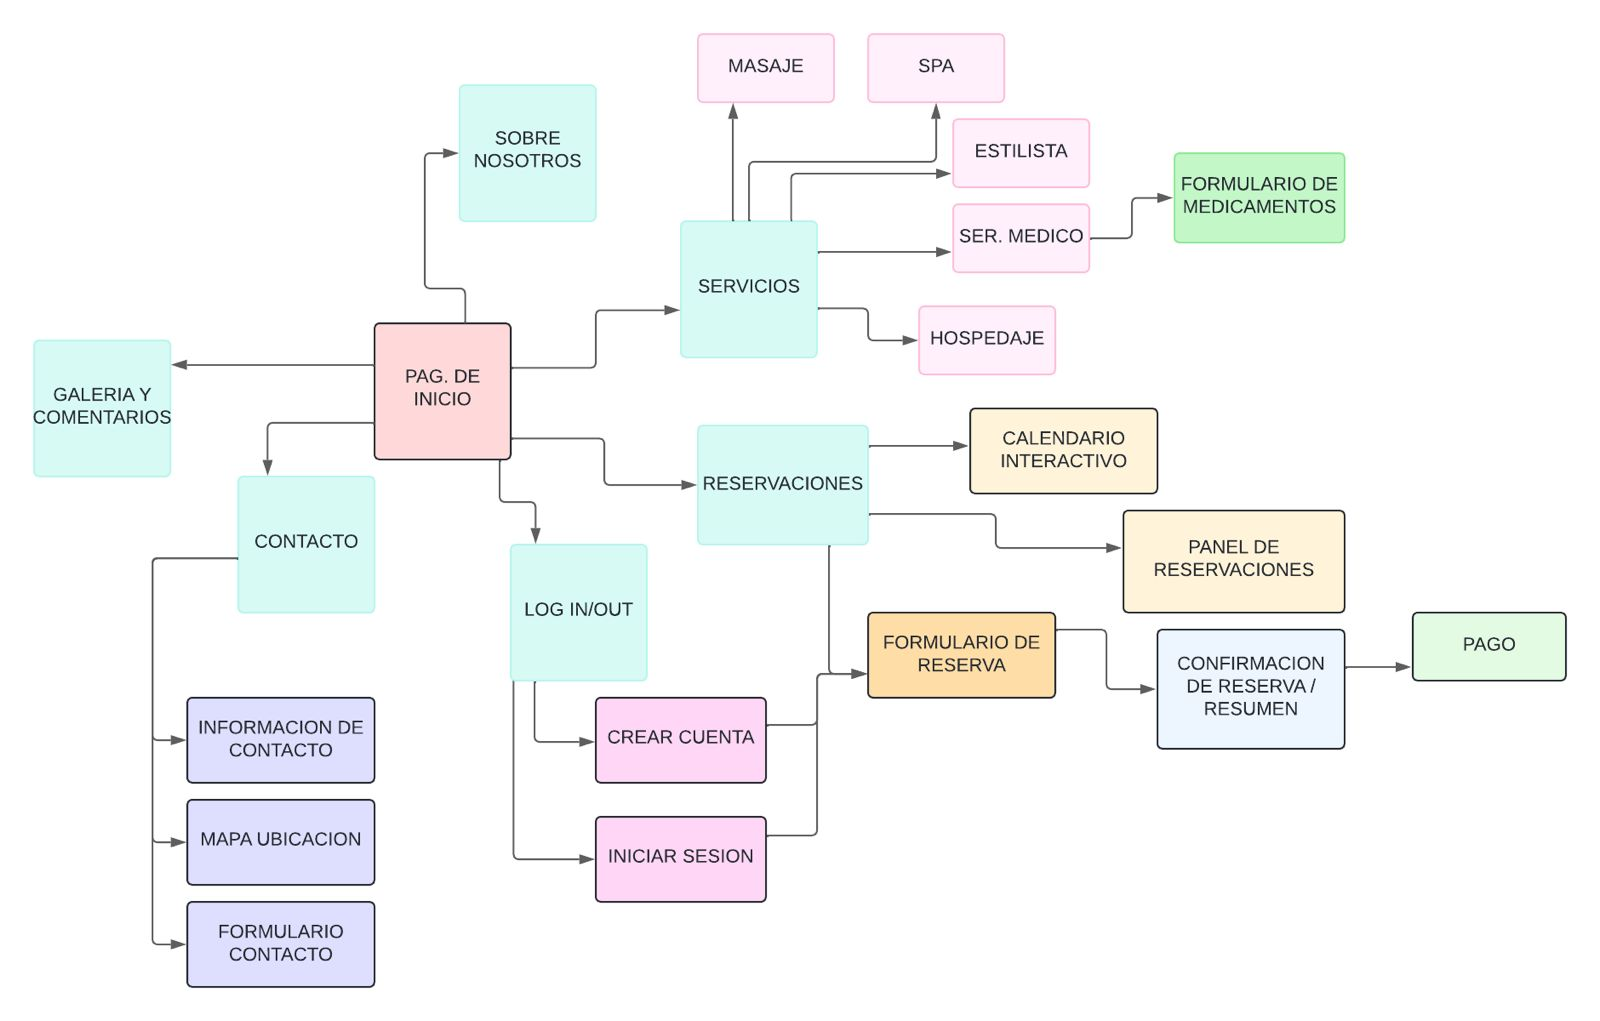
\includegraphics[width=.7\textwidth]{images/mapa_pethome}
		\caption{mapa}
		\label{fig:mapa}
	\end{center}
\end{figure}


\cdtInstrucciones{A continuación describa cada una de las pantallas.}
%% !TeX root = ../proyecto.tex
%--------------------------------------
\section{IUX Interfaz (nombre de la interfaz)}

\subsection{Objetivo}
	\cdtInstrucciones{Describa el objetivo, propósito o función de la pantalla.}

\subsection{Diseño}
	\cdtInstrucciones{Describa brevemente los elementos de la pantalla y como de be usarse a manera de manual de usuario.} Esta pantalla \IUref{IU23}{Pantalla de Control de Acceso} aparece al iniciar el sistema, para ingresar ... 

\IUfig[.7]{Login}{IU23}{Pantalla de Control de Acceso.}

%\IUfig[ancho de la figura: valor entre 1 y .1]{Nombre corto de la pantalla sin espacions ni acentos}{IUXX}{Nombre largo de la pantalla.}

\subsection{Salidas}

	\cdtInstrucciones{Liste las salidas de la interfaz. Si coinciden con las del caso de uso solo indiquelo. Esta ,ista debe incluir los mensajes}

	\begin{itemize}
		\item Descripción de salida.
	\end{itemize}
	
\subsection{Entradas}

	\cdtInstrucciones{Liste las entradas de la interfaz. Si coinciden con las del caso de uso solo indiquelo.}
	\begin{itemize}
		\item Descripción de salida.
	\end{itemize}

\subsection{Comandos}
	\cdtInstrucciones{Describa cada control (botónes, areas de drag and drop, componentes interactivos, animaciones, etc.) que se puede utilizar dentro de la pantalla indicando o que hacen y si cambia de pantalla.}

\begin{itemize}
	\item \IUbutton{Entrar}: Verifica que el Estudiante se encuentre registrado y la contraseña sea la correcta. Si la verificación es correcta, se muestra la \IUref{UI32}{Pantalla de Selección de Seminario}.
	\item \IUbutton{Ayuda}: Muestra la ayuda de esta pantalla \IUref{IU50}{Pantalla de Ayuda}.
\end{itemize}


% !TeX root = ../proyecto.tex
%--------------------------------------
\section{IU1 Registrar Cliente}

\subsection{Objetivo}
	\cdtInstrucciones  El objetivo de esta pantalla es permitir al cliente capturar sus datos personales, registrarse en el sistema y poder acceder a las operaciones del sistema definidas para su perfil .


\subsection{Diseño}
	\cdtInstrucciones Esta pantalla \IUref{IU1}{Registrar Cliente} aparece cuando el cliente solicite registarse, para ingresar sus datos personales basta con llenar la informacion desde teclado o mouse, una vez llenados todos los datos podemos hacer click en el boton \IUbutton{Registrar} . 

\IUfig[.7]{RegistroCliente}{IU1}{Registrar Cliente.}

%\IUfig[ancho de la figura: valor entre 1 y .1]{Nombre corto de la pantalla sin espacions ni acentos}{IUXX}{Nombre largo de la pantalla.}

\subsection{Salidas}

	

	\begin{itemize}
		\item Las salidas son las mismas que las del caso de uso \hyperlink{CU1}{CU1 Registrar Cliente}.
	\end{itemize}
	
\subsection{Entradas}

	\cdtInstrucciones{Liste las entradas de la interfaz. Si coinciden con las del caso de uso solo indiquelo.}
	\begin{itemize}
		\item Las entradas son las mismas que las del caso de uso \hyperlink{CU1}{CU1 Registrar Cliente}.
	\end{itemize}

\subsection{Comandos}
	\cdtInstrucciones{Describa cada control (botónes, areas de drag and drop, componentes interactivos, animaciones, etc.) que se puede utilizar dentro de la pantalla indicando o que hacen y si cambia de pantalla.}

\begin{itemize}
	\item \IUbutton{Registrar}: Verifica que los datos personales hayan sido llenados correctamente. Si la verificación es correcta, se muestra la \IUref{UI5}{Pantalla de Home Cliente sin reservaciones}.
	\item \IUbutton{Iniciar sesion}: Muestra la patalla \IUref{IU1.2}{Iniciar sesion}.
\end{itemize}


% !TeX root = ../proyecto.tex
%--------------------------------------
\section{IU2 Pantalla de Datos Obligatorios de la Mascota }

\subsection{Objetivo}
	\cdtInstrucciones El objetivo de esta pantalla es permitir al usuario capturar los datos que son obligatorios de su mascota.

\subsection{Diseño}
	\cdtInstrucciones Esta pantalla \IUref{IU2}{Registrar Mascota} aparece al momento de querer hacer una reservacion, para ingresar los datos de la mascota basta con llenar la informacion desde teclado o mouse, una vez llenados todos los datos podemos hacer click en el boton \IUbutton{Registrar}   

\IUfig[.7]{registrarMascota}{IU2}{Registrar Mascota}

%\IUfig[ancho de la figura: valor entre 1 y .1]{Nombre corto de la pantalla sin espacions ni acentos}{IUXX}{Nombre largo de la pantalla.}

\subsection{Salidas}

	\begin{itemize}
		\item Si los datos de esta pantalla no son llenados, al momento de dar click en el boton \IUbutton{Siguiente}, saltara el mensaje \MSGref{MSG-001}{Campo obligatorio}.
	\end{itemize}
	
\subsection{Entradas}
	\begin{itemize}
		\item Las entradas son las del caso de uso \hyperlink{CU3}{CU3 Registrar Mascota}.
		\item Nombre de la Mascota
		\item Tamaño
		\item Fecha de nacimiento
		\item Especie
		\item Raza
		\item Color de la Mascota
		\item RUAC
		\item Vacunas
	\end{itemize}

\subsection{Comandos}
	%\cdtInstrucciones{Describa cada control (botónes, areas de drag and drop, componentes interactivos, animaciones, etc.) que se puede utilizar dentro de la pantalla indicando o que hacen y si cambia de pantalla.}

\begin{itemize}
	\item \IUbutton{Siguiente}: Verifica que los datos hayan sido llenados. Si la verificación es correcta, se muestra la \IUref{UI3}{Pantalla de Datos Extra de la Mascota}.
\end{itemize}


% !TeX root = ../proyecto.tex
%--------------------------------------
\section{IU2 Pantalla de Datos Obligatorios de la Mascota }

\subsection{Objetivo}
	\cdtInstrucciones El objetivo de esta pantalla es permitir al usuario capturar los datos que son obligatorios de su mascota.

\subsection{Diseño}
	\cdtInstrucciones Esta pantalla \IUref{IU3}{Registrar Mascota} aparece al momento de querer hacer una reservacion, para ingresar los datos de la mascota basta con llenar la informacion desde teclado o mouse, una vez llenados todos los datos podemos hacer click en el boton \IUbutton{Registrar}   

\IUfig[.7]{RegistrarDatosMascota}{IU3}{Registrar Datos Mascota}

%\IUfig[ancho de la figura: valor entre 1 y .1]{Nombre corto de la pantalla sin espacions ni acentos}{IUXX}{Nombre largo de la pantalla.}

\subsection{Salidas}

	\begin{itemize}
		\item Si los datos de esta pantalla no son llenados, al momento de dar click en el boton \IUbutton{Siguiente}, saltara el mensaje \MSGref{MSG-001}{Campo obligatorio}.
	\end{itemize}
	
\subsection{Entradas}
	\begin{itemize}
		\item Las entradas son las del caso de uso \hyperlink{CU3}{CU3 Registrar Mascota}.
		\item Nombre de la Mascota
		\item Tamaño
		\item Fecha de nacimiento
		\item Especie
		\item Raza
		\item Color de la Mascota
		\item RUAC
		\item Vacunas
	\end{itemize}

\subsection{Comandos}
	%\cdtInstrucciones{Describa cada control (botónes, areas de drag and drop, componentes interactivos, animaciones, etc.) que se puede utilizar dentro de la pantalla indicando o que hacen y si cambia de pantalla.}

\begin{itemize}
	\item \IUbutton{Siguiente}: Verifica que los datos hayan sido llenados. Si la verificación es correcta, se muestra la \IUref{UI3}{Pantalla de Datos Extra de la Mascota}.
\end{itemize}


% !TeX root = ../proyecto.tex
%--------------------------------------
\section{IUX Interfaz (nombre de la interfaz)}

\subsection{Objetivo}
	\cdtInstrucciones{Describa el objetivo, propósito o función de la pantalla.}

\subsection{Diseño}
	\cdtInstrucciones{Describa brevemente los elementos de la pantalla y como de be usarse a manera de manual de usuario.} Esta pantalla \IUref{IU23}{Pantalla de Control de Acceso} aparece al iniciar el sistema, para ingresar ... 

\IUfig[.7]{mainPage}{IU3}{Pantalla de inicio.}

%\IUfig[ancho de la figura: valor entre 1 y .1]{Nombre corto de la pantalla sin espacions ni acentos}{IUXX}{Nombre largo de la pantalla.}

\subsection{Salidas}

	\cdtInstrucciones{Liste las salidas de la interfaz. Si coinciden con las del caso de uso solo indiquelo. Esta ,ista debe incluir los mensajes}

	\begin{itemize}
		\item Descripción de salida.
	\end{itemize}
	
\subsection{Entradas}

	\cdtInstrucciones{Liste las entradas de la interfaz. Si coinciden con las del caso de uso solo indiquelo.}
	\begin{itemize}
		\item Descripción de salida.
	\end{itemize}

\subsection{Comandos}
	\cdtInstrucciones{Describa cada control (botónes, areas de drag and drop, componentes interactivos, animaciones, etc.) que se puede utilizar dentro de la pantalla indicando o que hacen y si cambia de pantalla.}

\begin{itemize}
	\item \IUbutton{Entrar}: Verifica que el Estudiante se encuentre registrado y la contraseña sea la correcta. Si la verificación es correcta, se muestra la \IUref{UI32}{Pantalla de Selección de Seminario}.
	\item \IUbutton{Ayuda}: Muestra la ayuda de esta pantalla \IUref{IU50}{Pantalla de Ayuda}.
\end{itemize}


% !TeX root = ../proyecto.tex
%--------------------------------------
\section{IU5 Pantalla Home Cliente}

\subsection{Objetivo}
	\cdtInstrucciones El objetivo de esta pantalla es permitir al cliente ver sus reservacionses, para que de esta forma tenga la opcion de editarlas o eliminarlas, y tambien que tenga la opcion de hacer una reservacion .

\subsection{Diseño}
	\cdtInstrucciones Esta pantalla {UI5}{Pantalla Home Cliente} aparece al momento de registrarse o iniciar sesion, una vez dentro tenemos la opcion de hacer una reservacion dando click en el boton \IUbutton{Reservar}, asi como visualizar nuestras reservaciones y tener la opcion de editar o eliminar la reservacion con los botones \IUbutton{Editar},\IUbutton{Eliminar}.

\IUfig[.7]{Reservaciones}{IU5}{Pantalla de Home Cliente}
\IUfig[.7]{sinReservaciones}{IU5}{Pantalla de Home Cliente sin reservaciones}

%\IUfig[ancho de la figura: valor entre 1 y .1]{Nombre corto de la pantalla sin espacions ni acentos}{IUXX}{Nombre largo de la pantalla.}

\subsection{Salidas}

	%\cdtInstrucciones{Liste las salidas de la interfaz. Si coinciden con las del caso de uso solo indiquelo. Esta ,ista debe incluir los mensajes}

	\begin{itemize}
		\item Si no se ha echo ninguna reservacion, se mostrara el mensaje \MSGref{MSG-003}{No hay reservaciones todavia}.
	\end{itemize}
	
\subsection{Entradas}

	%\cdtInstrucciones{Liste las entradas de la interfaz. Si coinciden con las del caso de uso solo indiquelo.}
	\begin{itemize}
		\item Ninguna
	\end{itemize}

\subsection{Comandos}
	%\cdtInstrucciones{Describa cada control (botónes, areas de drag and drop, componentes interactivos, animaciones, etc.) que se puede utilizar dentro de la pantalla indicando o que hacen y si cambia de pantalla.}

\begin{itemize}
	\item \IUbutton{Hacer reservacion}: Muestra la pantalla \IUref{UI2}{Pantalla de Datos Obligatorios de la Mascota}.
	\item \IUbutton{Editar}: Muestra la pantalla \IUref{UI2}{Pantalla de Datos Obligatorios de la Mascota}, con los datos de esa reservacion y permite modificarlos.
	\item \IUbutton{Eliminar}: Elimina la reservación.
\end{itemize}


% !TeX root = ../proyecto.tex
%--------------------------------------
\section{IU6 Interfaz búsqueda de hospedajes}

\subsection{Objetivo}
	\cdtInstrucciones{Describa el objetivo, propósito o función de la pantalla.}

\subsection{Diseño}
	\cdtInstrucciones{Describa brevemente los elementos de la pantalla y como de be usarse a manera de manual de usuario.} Esta pantalla \IUref{IU23}{Pantalla de Control de Acceso} aparece al iniciar el sistema, para ingresar ... 

\IUfig[0.8]{PANTALLA_BUSQUEDA_HOSPEDAJES}{IU6}{Búsqueda de hospedajes.}

\subsection{Salidas}

	\cdtInstrucciones{Liste las salidas de la interfaz. Si coinciden con las del caso de uso solo indiquelo. Esta ,ista debe incluir los mensajes}

	\begin{itemize}
		\item Descripción de salida.
	\end{itemize}
	
\subsection{Entradas}

	\cdtInstrucciones{Liste las entradas de la interfaz. Si coinciden con las del caso de uso solo indiquelo.}
	\begin{itemize}
		\item Descripción de salida.
	\end{itemize}

\subsection{Comandos}
	\cdtInstrucciones{Describa cada control (botónes, areas de drag and drop, componentes interactivos, animaciones, etc.) que se puede utilizar dentro de la pantalla indicando o que hacen y si cambia de pantalla.}

\begin{itemize}
	\item \IUbutton{Entrar}: Verifica que el Estudiante se encuentre registrado y la contraseña sea la correcta. Si la verificación es correcta, se muestra la \IUref{UI32}{Pantalla de Selección de Seminario}.
	\item \IUbutton{Ayuda}: Muestra la ayuda de esta pantalla \IUref{IU50}{Pantalla de Ayuda}.
\end{itemize}


% !TeX root = ../proyecto.tex
%--------------------------------------
\section{IU7 Interfaz catálogo de habitaciones}

\subsection{Objetivo}
	\cdtInstrucciones{Describa el objetivo, propósito o función de la pantalla.}

\subsection{Diseño}
	\cdtInstrucciones{Describa brevemente los elementos de la pantalla y como de be usarse a manera de manual de usuario.} Esta pantalla \IUref{IU23}{Pantalla de Control de Acceso} aparece al iniciar el sistema, para ingresar ... 

\IUfig[.8]{PANTALLA_CATALOGO_HABITACIONES}{IU7}{Pantalla de catálogo de habitaciones.}

%\IUfig[ancho de la figura: valor entre 1 y .1]{Nombre corto de la pantalla sin espacions ni acentos}{IUXX}{Nombre largo de la pantalla.}

\subsection{Salidas}

	\cdtInstrucciones{Liste las salidas de la interfaz. Si coinciden con las del caso de uso solo indiquelo. Esta lista debe incluir los mensajes}

	\begin{itemize}
		\item Descripción de salida.
	\end{itemize}
	
\subsection{Entradas}

	\cdtInstrucciones{Liste las entradas de la interfaz. Si coinciden con las del caso de uso solo indiquelo.}
	\begin{itemize}
		\item Descripción de salida.
	\end{itemize}

\subsection{Comandos}
	\cdtInstrucciones{Describa cada control (botónes, areas de drag and drop, componentes interactivos, animaciones, etc.) que se puede utilizar dentro de la pantalla indicando o que hacen y si cambia de pantalla.}

\begin{itemize}
	\item \IUbutton{Entrar}: Verifica que el Estudiante se encuentre registrado y la contraseña sea la correcta. Si la verificación es correcta, se muestra la \IUref{UI32}{Pantalla de Selección de Seminario}.
	\item \IUbutton{Ayuda}: Muestra la ayuda de esta pantalla \IUref{IU50}{Pantalla de Ayuda}.
\end{itemize}
% !TeX root = ../proyecto.tex
%--------------------------------------
\section{IU8 Interfaz vista general del cuarto}

\subsection{Objetivo}
	\cdtInstrucciones{Describa el objetivo, propósito o función de la pantalla.}

\subsection{Diseño}
	\cdtInstrucciones{Describa brevemente los elementos de la pantalla y como de be usarse a manera de manual de usuario.} Esta pantalla \IUref{IU23}{Pantalla de Control de Acceso} aparece al iniciar el sistema, para ingresar ... 

\IUfig[.8]{PANTALLA_VISTA_GENERAL}{IU8}{Pantalla de vista general del cuarto.}

%\IUfig[ancho de la figura: valor entre 1 y .1]{Nombre corto de la pantalla sin espacions ni acentos}{IUXX}{Nombre largo de la pantalla.}

\subsection{Salidas}

	\cdtInstrucciones{Liste las salidas de la interfaz. Si coinciden con las del caso de uso solo indiquelo. Esta ,ista debe incluir los mensajes}

	\begin{itemize}
		\item Descripción de salida.
	\end{itemize}
	
\subsection{Entradas}

	\cdtInstrucciones{Liste las entradas de la interfaz. Si coinciden con las del caso de uso solo indiquelo.}
	\begin{itemize}
		\item Descripción de salida.
	\end{itemize}

\subsection{Comandos}
	\cdtInstrucciones{Describa cada control (botónes, areas de drag and drop, componentes interactivos, animaciones, etc.) que se puede utilizar dentro de la pantalla indicando o que hacen y si cambia de pantalla.}

\begin{itemize}
	\item \IUbutton{Entrar}: Verifica que el Estudiante se encuentre registrado y la contraseña sea la correcta. Si la verificación es correcta, se muestra la \IUref{UI32}{Pantalla de Selección de Seminario}.
	\item \IUbutton{Ayuda}: Muestra la ayuda de esta pantalla \IUref{IU50}{Pantalla de Ayuda}.
\end{itemize}


% !TeX root = ../proyecto.tex
%--------------------------------------
\section{IU9 Interfaz servicios adicionales}

\subsection{Objetivo}
	\cdtInstrucciones{Describa el objetivo, propósito o función de la pantalla.}

\subsection{Diseño}
	\cdtInstrucciones{Describa brevemente los elementos de la pantalla y como de be usarse a manera de manual de usuario.} Esta pantalla \IUref{IU23}{Pantalla de Control de Acceso} aparece al iniciar el sistema, para ingresar ... 

\IUfig[.7]{PANTALLA_SERVICIOS_EXTRA}{IU9}{Pantalla de servicios adicionales.}

%\IUfig[ancho de la figura: valor entre 1 y .1]{Nombre corto de la pantalla sin espacions ni acentos}{IUXX}{Nombre largo de la pantalla.}

\subsection{Salidas}

	\cdtInstrucciones{Liste las salidas de la interfaz. Si coinciden con las del caso de uso solo indiquelo. Esta ,ista debe incluir los mensajes}

	\begin{itemize}
		\item Descripción de salida.
	\end{itemize}
	
\subsection{Entradas}

	\cdtInstrucciones{Liste las entradas de la interfaz. Si coinciden con las del caso de uso solo indiquelo.}
	\begin{itemize}
		\item Descripción de salida.
	\end{itemize}

\subsection{Comandos}
	\cdtInstrucciones{Describa cada control (botónes, areas de drag and drop, componentes interactivos, animaciones, etc.) que se puede utilizar dentro de la pantalla indicando o que hacen y si cambia de pantalla.}

\begin{itemize}
	\item \IUbutton{Entrar}: Verifica que el Estudiante se encuentre registrado y la contraseña sea la correcta. Si la verificación es correcta, se muestra la \IUref{UI32}{Pantalla de Selección de Seminario}.
	\item \IUbutton{Ayuda}: Muestra la ayuda de esta pantalla \IUref{IU50}{Pantalla de Ayuda}.
\end{itemize}


% !TeX root = ../proyecto.tex
%--------------------------------------
\section{IU10 Interfaz registrar más detalles}

\subsection{Objetivo}
	\cdtInstrucciones{Describa el objetivo, propósito o función de la pantalla.}

\subsection{Diseño}
	\cdtInstrucciones{Describa brevemente los elementos de la pantalla y como de be usarse a manera de manual de usuario.} Esta pantalla \IUref{IU23}{Pantalla de Control de Acceso} aparece al iniciar el sistema, para ingresar ... 

\IUfig[.8]{PANTALLA_REGISTRAR_MAS_DETALLES}{IU10}{Pantalla de registrar más detalles.}

%\IUfig[ancho de la figura: valor entre 1 y .1]{Nombre corto de la pantalla sin espacions ni acentos}{IUXX}{Nombre largo de la pantalla.}

\subsection{Salidas}

	\cdtInstrucciones{Liste las salidas de la interfaz. Si coinciden con las del caso de uso solo indiquelo. Esta ,ista debe incluir los mensajes}

	\begin{itemize}
		\item Descripción de salida.
	\end{itemize}
	
\subsection{Entradas}

	\cdtInstrucciones{Liste las entradas de la interfaz. Si coinciden con las del caso de uso solo indiquelo.}
	\begin{itemize}
		\item Descripción de salida.
	\end{itemize}

\subsection{Comandos}
	\cdtInstrucciones{Describa cada control (botónes, areas de drag and drop, componentes interactivos, animaciones, etc.) que se puede utilizar dentro de la pantalla indicando o que hacen y si cambia de pantalla.}

\begin{itemize}
	\item \IUbutton{Entrar}: Verifica que el Estudiante se encuentre registrado y la contraseña sea la correcta. Si la verificación es correcta, se muestra la \IUref{UI32}{Pantalla de Selección de Seminario}.
	\item \IUbutton{Ayuda}: Muestra la ayuda de esta pantalla \IUref{IU50}{Pantalla de Ayuda}.
\end{itemize}


% !TeX root = ../proyecto.tex
%--------------------------------------
\section{IU11 Interfaz resumen del hospedaje}

\subsection{Objetivo}
	\cdtInstrucciones{Describa el objetivo, propósito o función de la pantalla.}

\subsection{Diseño}
	\cdtInstrucciones{Describa brevemente los elementos de la pantalla y como de be usarse a manera de manual de usuario.} Esta pantalla \IUref{IU23}{Pantalla de Control de Acceso} aparece al iniciar el sistema, para ingresar ... 

\IUfig[.7]{RESUMEN_HOSPEDAJE}{IU11}{Pantalla de resumen del hospedaje.}

%\IUfig[ancho de la figura: valor entre 1 y .1]{Nombre corto de la pantalla sin espacions ni acentos}{IUXX}{Nombre largo de la pantalla.}

\subsection{Salidas}

	\cdtInstrucciones{Liste las salidas de la interfaz. Si coinciden con las del caso de uso solo indiquelo. Esta ,ista debe incluir los mensajes}

	\begin{itemize}
		\item Descripción de salida.
	\end{itemize}
	
\subsection{Entradas}

	\cdtInstrucciones{Liste las entradas de la interfaz. Si coinciden con las del caso de uso solo indiquelo.}
	\begin{itemize}
		\item Descripción de salida.
	\end{itemize}

\subsection{Comandos}
	\cdtInstrucciones{Describa cada control (botónes, areas de drag and drop, componentes interactivos, animaciones, etc.) que se puede utilizar dentro de la pantalla indicando o que hacen y si cambia de pantalla.}

\begin{itemize}
	\item \IUbutton{Entrar}: Verifica que el Estudiante se encuentre registrado y la contraseña sea la correcta. Si la verificación es correcta, se muestra la \IUref{UI32}{Pantalla de Selección de Seminario}.
	\item \IUbutton{Ayuda}: Muestra la ayuda de esta pantalla \IUref{IU50}{Pantalla de Ayuda}.
\end{itemize}




%!TEX root = ejemplo.tex
%=========================================================
\section{Catálogo de mensajes}	
\label{sec:mensajes}

	En esta sección se describen todos los mensajes que aparecen en el sistema. Para cada mensaje se especifica:
	 
	\begin{description}\itemsep0em
		\item[Id:] Identificador del mensaje de la forma ``MSG XX'' y descripción corta del mismo.
		\item[Tipo:] Tipo del mensaje el cual puede ser: 
		\begin{description}
			\item[Normal:] Mensaje que informa al usuario una instrucción o el estado interno que guarda el sistema, suele tener un color {\color{msgNormalColor}Azul}.
			\item[Éxito:] Mensaje que informa al usuario sobre una acción realizada, sirve para confirmar el correcto funcionamiento del sistema. Se presentan con un color {\color{msgInfoColor}Verde}.
			\item[Atención:] Mensaje que tiene como finalidad llamar la atención del usuario a una situación que requiere su intervención, por ejemplo cuando una actividad ha generado un efecto colateral o se realizará una acción destructiva y no reversible. Se presentan con un color {\color{msgWarningColor}Naranja}.
			\item[Error:] Mensaje que informa al usuario un fallo en en una operación o un impedimento para realizarla, por ejemplo: cuando no se puede efectuar la acción solicitada, cuando un dato falta o tiene un formato no aceptado por el sistema. Se presentan con un color {\color{msgErrorColor}Rojo}.
		\end{description}
		\item[Propósito:] Explicación del propósito del mensaje.
		\item[Redacción:] Redacción del mensaje.
		\item[Parámetros:] En caso de que el mensaje pueda variar se especifican los casos y la forma en que debe adaptarse la redacción
		\item[Ejemplos:] Ejemplos de como debe renderizarse el mensaje.
	\end{description}


\subsection{Lista de mensajes}
%msgNormalColor
%msgInfoColor
%msgWarninigColor
%msgErrorColor

%Mensaje establecido y en uso
\begin{cdtMessage}[msgErrorColor]{MSG-001}{Campo obligatorio}
	\item[Propósito:] Indicar al usuario que existen campos vacíos en su petición que son obligatorios para completar con éxito la operación
	\item[Redacción:] El campo "$<$atributo$>$" debe ser llenado para continuar.
	\item[Parámetros:] \hspace{1cm}
	\begin{itemize}
		\item $<$atributo$>$ se refiere al nombre del atributo que se está dejando vacío en la petición.
	\end{itemize}
	\item[Ejemplos:] El campo $"$CURP$"$ debe ser llenado para continuar.
\end{cdtMessage}

%Mensaje sin establecer ni usar
\begin{cdtMessage}[msgErrorColor]{MSG-002}{RUAC ya existente} 
	\item[Propósito:] Indicar al usuario que el RUAC ingresado para la mascota ya se encuentra asociado a otra en el sistema.
	\item[Redacción:] El RUAC $<$RUAC$>$ ya se encuentra asociado a otra mascota.
	\item[Parámetros:] \hspace{1cm}
	\begin{itemize}
		\item $<$RUAC$>$ Se refiere al \hyperlink{mascota.RUAC}{RUAC} que el usuario desea asociar a su mascota.
	\end{itemize}
	\item[Ejemplos:] El RUAC PHCXA50604 ya se encuentra asociado a otra mascota.
\end{cdtMessage}

%Mensaje establecido y en uso
\begin{cdtMessage}[msgErrorColor]{MSG-003}{No hay reservaciones} 
	\item[Propósito:] Indicar al cliente que no tiene reservaciones realizadas o sin pagar.
	\item[Redacción:] No tienes reservaciones. ¿Deseas realizar una?.
	\item[Parámetros:] No aplica.
	\item[Ejemplos:] No tienes reservaciones. ¿Deseas realizar una?.
\end{cdtMessage}

%Mensaje establecido y en uso
\begin{cdtMessage}[msgErrorColor]{MSG-004}{Vacunas obligatorias}
	\item[Propósito:] Indicar al usuario que para poder registrar a su mascota y sea aceptada para hospedarse en el hotel debe contar con las 3 vacunas mínimas obligatorias.
	\item[Redacción:] Por tu seguridad y la de los demás, tu mascota debe contar con las 3 vacunas mínimas obligatotias.
	\item[Parámetros:] No aplica.
	\item[Ejemplos:] Por tu seguridad y la de los demás, tu mascota debe contar con las 3 vacunas mínimas obligatotias.
\end{cdtMessage}

%Mensaje establecido y en uso
\begin{cdtMessage}[msgErrorColor]{MSG-005}{CURP ya existente}
	\item[Propósito:] Indica al usuario que el CURP con el que intenta registrarse ya es ocupado por otro perfil.
	\item[Redacción:] El CURP introducido ya está registrado en otro perfil.
	\item[Parámetros:] No aplica.
	\item[Ejemplos:] El CURP introducido ya está registrado en otro perfil.
\end{cdtMessage}

%Mensaje establecido y en uso
\begin{cdtMessage}[msgErrorColor]{MSG-006}{Correo electrónico ya existente}
	\item[Propósito:] Indicar al usuario que el correo electrónico con el que intenta registrarse ya es ocupado por otro perfil.
	\item[Redacción:] El correo electrónico introducido ya está registrado en otro perfil.
	\item[Parámetros:] No aplica.
	\item[Ejemplos:] El correo electrónico introducido ya está registrado en otro perfil.
\end{cdtMessage}

%Mensaje establecido y en uso
\begin{cdtMessage}[msgErrorColor]{MSG-007}{Dato no válido}
	\item[Propósito:] Indicar al usuario que uno o más campos están siendo llenados con formatos no válidos en su solicitud para poder realizar con éxito la operación.
	\item[Redacción:] Introduzca valores válidos en los campos correspondientes.
	\item[Parámetros:] No aplica.
	\item[Ejemplos:] Introduzca valores válidos en los campos correspondientes.
\end{cdtMessage}

%Mensaje establecido y en uso
\begin{cdtMessage}[msgErrorColor]{MSG-008}{Fecha no disponible} 
	\item[Propósito:] Indicar al usuario que en las fechas que selecciona su hospedaje no hay cuartos disponibles con las características solicitadas.
	\item[Redacción:] Lo sentimos, no hay cuartos disponibles para el periodo del $<$check-in$>$ al $<$check-out$>$ con las características requeridas. Seleccione otro periodo. 
	\item[Parámetros:] \hspace{1cm}
	\begin{itemize}
		\item $<$check-in$>$ Fecha proyectada de llegada y en la que se inicia el periodo de hospedaje.
		\item $<$check-out$>$ Fecha proyectada de salida y en la que se finaliza el periodo de hospedaje.
	\end{itemize}
	\item[Ejemplos:] \hspace{1cm}
	\begin{itemize}
		\item Lo sentimos, no hay cuartos disponibles para el periodo del 07-05-2024 al 09-05-2024 con las características requeridas. Seleccione otro periodo. 
	\end{itemize}
\end{cdtMessage}


\end{document}
